
%%%%%%%%%%%%%%%%%%%%%%%%%%%%%%%%%%%%%%%%%%%%%%%%%%%%%%%%%%%%%%%%%%%%%%%%%%%%%%
% Copyright (c) 2003-2014 by University of Queensland
% http://www.uq.edu.au
%
% Primary Business: Queensland, Australia
% Licensed under the Open Software License version 3.0
% http://www.opensource.org/licenses/osl-3.0.php
%
% Development until 2012 by Earth Systems Science Computational Center (ESSCC)
% Development 2012-2013 by School of Earth Sciences
% Development from 2014 by Centre for Geoscience Computing (GeoComp)
%
%%%%%%%%%%%%%%%%%%%%%%%%%%%%%%%%%%%%%%%%%%%%%%%%%%%%%%%%%%%%%%%%%%%%%%%%%%%%%%

\documentclass{esysdoc}
\usepackage{color}

%%%%%%%%%%%%%%%%%%%%%%%%%%%%%%%%%%%%%%%%%%%%%%%%%%%%%%%%%%%%%%%%%%%%%%%%%%%%%%
% Copyright (c) 2003-2015 by University of Queensland
% http://www.uq.edu.au
%
% Primary Business: Queensland, Australia
% Licensed under the Open Software License version 3.0
% http://www.opensource.org/licenses/osl-3.0.php
%
% Development until 2012 by Earth Systems Science Computational Center (ESSCC)
% Development 2012-2013 by School of Earth Sciences
% Development from 2014 by Centre for Geoscience Computing (GeoComp)
%
%%%%%%%%%%%%%%%%%%%%%%%%%%%%%%%%%%%%%%%%%%%%%%%%%%%%%%%%%%%%%%%%%%%%%%%%%%%%%%

\usepackage{listing}
% defines the colour for the background of code examples
\definecolor{LightGrey}{gray}{0.9}

%Some colour definitions added to keep pdflatex happy
%I make no claim that these values are particularly good
\definecolor{Purple}{rgb}{0.7, 0, 0.6}
\definecolor{Tan}{rgb}{0.5,0.5,0.5}
\definecolor{BrickRed}{rgb}{0.7, 0.2, 0.2}
\definecolor{Black}{rgb}{0, 0, 0}

% All the \color{x} used to be \color[named]{x}
%end color defs

\lstdefinestyle{myC++}{%
language=C++,
showstringspaces=false,
basicstyle=\small\ttfamily,
commentstyle=\color{BrickRed}\ttfamily,
keywordstyle=\color{Purple}\ttfamily,
%identifierstyle=\color{Blue}\ttfamily,
%functionstyle=\color{Blue}\ttfamily,
%typestyle=\color{ForestGreen}\ttfamily,
stringstyle=\color{Tan}\ttfamily,%
morekeywords={,complex,}%
frame=none,%
backgroundcolor=\color{LightGrey}%
}

\lstdefinestyle{myMatlab}{%
language=Matlab,
showstringspaces=false,
basicstyle=\small\ttfamily,
commentstyle=\color{BrickRed}\ttfamily,
keywordstyle=\color{Purple}\ttfamily,
%identifierstyle=\color{Blue}\ttfamily,
%functionstyle=\color{Blue}\ttfamily,
%typestyle=\color{ForestGreen}\ttfamily,
stringstyle=\color{Tan}\ttfamily,%
frame=none,%
backgroundcolor=\color{LightGrey}%
}

\lstdefinestyle{myScilab}{%
language=Scilab,
showstringspaces=false,
basicstyle=\small\ttfamily,
commentstyle=\color{BrickRed}\ttfamily,
keywordstyle=\color{Purple}\ttfamily,
%identifierstyle=\color{Blue}\ttfamily,
%functionstyle=\color{Blue}\ttfamily,
%typestyle=\color{ForestGreen}\ttfamily,
stringstyle=\color{Tan}\ttfamily,%
frame=none,%
backgroundcolor=\color{LightGrey}%
}

\lstdefinestyle{myShell}{%
language=ksh,
showstringspaces=false,
basicstyle=\small\ttfamily,
commentstyle=\color{Black}\ttfamily,
keywordstyle=\color{Black}\ttfamily,
%identifierstyle=\color{Blue}\ttfamily,
%functionstyle=\color{Blue}\ttfamily,
%typestyle=\color{ForestGreen}\ttfamily,
stringstyle=\color{Black}\ttfamily,%
frame=none,%
backgroundcolor=\color{LightGrey}%
}

\lstdefinestyle{myPython}{%
language=python,
showstringspaces=false,
basicstyle=\small\ttfamily,
commentstyle=\color{BrickRed}\ttfamily,
keywordstyle=\color{Purple}\ttfamily,
%identifierstyle=\color{Blue}\ttfamily,
%functionstyle=\color{Blue}\ttfamily,
%typestyle=\color{ForestGreen}\ttfamily,
stringstyle=\color{Tan}\ttfamily,%
frame=none,%
%backgroundcolor=\color{LightGrey}%
}

\lstdefinestyle{myhtml}{%
language=xml,
showstringspaces=false,
basicstyle=\small\ttfamily,
commentstyle=\color{BrickRed}\ttfamily,
keywordstyle=\color{Purple}\ttfamily,
%identifierstyle=\color{Blue}\ttfamily,
%functionstyle=\color{Blue}\ttfamily,
%typestyle=\color{ForestGreen}\ttfamily,
stringstyle=\color{Tan}\ttfamily,
morekeywords={,simulation,prop_dim,error_check,stochastic,%
  globals,field,dimensions,lattice,domains,samples,vector,%
  components,fourier_space,sequence,integrate,algorithm,%
  interval,k_operators,constant,operator_names,vectors,%
  output,filename,group,sampling,moments,benchmark,use_double,%
  use_wisdom,use_prefs,binary_output,cycles,filter,post_propagation,%
  default_value,argv,arg,iterations,cross_propagation,%
  use_mpi,paths,seed,noises,author,description,name,type,%
}
frame=none,%
%framerule=2pt,%
backgroundcolor=\color{LightGrey}%
}


% this implements producing nice code blocks
% it also saves time, typing and
% *should* reduce errors in the text by removing doubling up of code
\lstnewenvironment{xmdsCode}[1][]{\lstset{style=myhtml}\lstset{#1}}{}

% this implements nicely formatted shell code
\lstnewenvironment{shellCode}[1][]{\lstset{style=myShell}\lstset{#1}}{}

% this implements nicely formatted Perl code
\lstnewenvironment{perlCode}[1][]{\lstset{style=myPerl}\lstset{#1}}{}

% this implements nicely formatted Python code
\lstnewenvironment{python}[1][]{\lstset{style=myPython}\lstset{#1}}{}

% this implements nicely formatted C++ code
\lstnewenvironment{CCode}{\lstset{style=myC++}}{}

% this implements nicely formatted matlab code
\lstnewenvironment{matlabCode}{\lstset{style=myMatlab}}{}

% this implements nicely formatted scilab code
\lstnewenvironment{scilabCode}{\lstset{style=myScilab}}{}

\usepackage{makeidx}
\usepackage{program}
\usepackage{graphicx, subfigure}

\graphicspath{{figures/}}


%%%%%%%%%%%%%%%%%%%%%%%%%%%%%%%%%%%%%%%%%%%%%%%%%%%%%%%%%%%%%%%%%%%%%%%%%%%%%%
% Copyright (c) 2003-2015 by University of Queensland
% http://www.uq.edu.au
%
% Primary Business: Queensland, Australia
% Licensed under the Open Software License version 3.0
% http://www.opensource.org/licenses/osl-3.0.php
%
% Development until 2012 by Earth Systems Science Computational Center (ESSCC)
% Development 2012-2013 by School of Earth Sciences
% Development from 2014 by Centre for Geoscience Computing (GeoComp)
%
%%%%%%%%%%%%%%%%%%%%%%%%%%%%%%%%%%%%%%%%%%%%%%%%%%%%%%%%%%%%%%%%%%%%%%%%%%%%%%

\newtheorem{algorithm}{Algorithm}[chapter] 
\newtheorem{pyc}{Python Program}[chapter] 
\newcommand{\downunder}{\module{esys.downunder}\xspace}
\newcommand{\weipa}{\textit{esys.weipa}\xspace}
\newcommand{\escript}{\textit{escript}\xspace}
\newcommand{\Python}{\textit{python}\xspace}
\newcommand{\finley}{\textit{finley}\xspace}
\newcommand{\LinearPDE}{\texttt{LinearPDE}\xspace}
\newcommand{\Data}{\texttt{Data}\xspace}
\newcommand{\Domain}{\texttt{Domain}\xspace}
\newcommand{\argmin}{\mbox{arg}\min}
\newcommand{\True}{\constant{True}\xspace}
\newcommand{\False}{\constant{False}\xspace}
\newcommand{\None}{\constant{None}\xspace}
\newcommand{\dirac}{D}
\newcommand{\mat}[1]{\mathbf{#1}}
\newcommand{\examplefile}[1]{\texttt{#1}\xspace}
\newcommand{\netcdf}{\textit{netCDF}\xspace}
%\newcommand{\CIHAN}[1]{\textbf{CIHAN: #1} }
%\newcommand{\LG}[1]{\textbf{LG: #1} }
\newcommand{\VisIt}{{\it VisIt}\index{visualization!VisIt}\index{VisIt}\xspace}
\newcommand{\mayavi}{{\it mayavi}\index{visualization!mayavi}\index{mayavi}\xspace}
\newcommand{\GOCAD}{{\it GOCAD}\index{GOCAD}\xspace}
\newcommand{\VTK}{{\it VTK}\index{visualization!VTK}\index{VTK}\xspace}
\newcommand{\SILO}{{\it SILO}\index{visualization!SILO}\index{SILO}\xspace}
\newcommand{\CSV}{{\it CSV}\index{CSV}\xspace}
\newcommand{\Voxet}{{\it Voxet}\index{Voxet}\xspace}


\makeindex

\begin{document}

\pagestyle{empty} %No headings for the first pages.

\title{\downunder: Inversion with \escript}
\author{Cihan Altinay, Vince Boros, Lutz Gross, Azadeh Salehi}
\authoraddress{
The University of Queensland\\
School of Earth Sciences\\
St. Lucia, QLD 4072, Australia.}
%\release{3.4.1}
\release{development}

\maketitle

\begin{center}
Copyright (c) 2012--2014 by University of Queensland	\\
\url{http://www.uq.edu.au}				\\
Primary Business: Queensland, Australia			\\
Licensed under the Open Software License version 3.0	\\
\url{http://www.opensource.org/licenses/osl-3.0.php}	\\

This work is supported by the AuScope National Collaborative Research Infrastructure Strategy, 
the Queensland State Government and The University of Queensland.

\end{center}

\cleardoublepage\pdfbookmark[0]{Contents}{contents}%
\tableofcontents %Table of contents
\cleardoublepage %The first chapter should start on an odd page.

\pagestyle{fancy}
\phantomsection\addcontentsline{toc}{chapter}{Overview}
%%%%%%%%%%%%%%%%%%%%%%%%%%%%%%%%%%%%%%%%%%%%%%%%%%%%%%%%
%
% Copyright (c) 2003-2012 by University of Queensland
% Earth Systems Science Computational Center (ESSCC)
% http://www.uq.edu.au/esscc
%
% Primary Business: Queensland, Australia
% Licensed under the Open Software License version 3.0
% http://www.opensource.org/licenses/osl-3.0.php
%
%%%%%%%%%%%%%%%%%%%%%%%%%%%%%%%%%%%%%%%%%%%%%%%%%%%%%%%%

\chapter{Introduction}
This document describes how to install \emph{esys-Escript}\footnote{For the rest of the document we will drop the \emph{esys-}} on your computer.
To learn how to use \esfinley please see the Cookbook, User's guide or the API documentation.
If you use the Debian or Ubuntu packages to install then the documentation will be available in
\file{/usr/share/doc/escript}, otherwise (if you haven't done so already) you can download the documentation bundle 
from launchpad.

\esfinley is primarily developed on Linux desktop, SGI ICE and \macosx systems.
It is distributed in two forms:
\begin{enumerate}
  \item Binary bundles -- these are great for first time users or for those who want to start using 
    \esfinley immediately.
      Bundles are available for:
      \begin{itemize}
	  \item Debian and Ubuntu Linux distributions ($32$/$64$-bit i686) (.deb package)
	  \item Linux desktop systems with gcc (stand-alone bundle)
	  \item \macosx Leopard systems (also tested on Lion) with gcc (stand-alone bundle)
	  \item $32$bit Windows (requires some other packages to be installed).
      \end{itemize}    
    Please see Chapter~\ref{chap:bin} for instructions on how to install the binary bundles \esfinley.
  \item Source bundles -- these require compilation and should be used if the binary bundles 
    don't work on the target machine or if extra functionality is required such as \mpi parallelisation.
    See Chapter~\ref{chap:compiler} for detailed instructions.
\end{enumerate}

See the site \url{https://answers.launchpad.net/escript-finley} for online help.

\section{Significant changes since version 3.3}
\begin{itemize}
 \item \texttt{SymPy} is now required to compile or run \escript. 
    This means you will need to download sympy in addition to the support bundle from previous releases.
 \item The minimum Python version is now $2.6$.
\end{itemize}

% \noindent If you choose to compile from source your options are to
% \begin{itemize}
%     \item install dependencies (e.g. using your package manager) and only compile \esfinley, OR
%     \item compile everything from source.
% \end{itemize}
% Either way, please see Chapter~\ref{chap:compiler} for a discussion of compiler features.
% Compiling \esfinley when its dependencies are already installed is discussed in Chapter~\ref{chap:essrc}.
% To compile \esfinley and all dependencies from source please see Chapter~\ref{chap:allsrc}.
% The latter option takes a significant amount of time and is only required if the versions of the dependent libraries available on your system do not work with \esfinley.
% 
% Once everything is installed you can test your installation using the Python scripts in \file{examples.zip} or \file{examples.tar.gz}\footnote{These should either be in \file{escript.d/release/doc} or in the case of Debian, in \file{/usr/share/doc/escript}.}.
% Unpack the examples and try to run the following from a terminal:
% \begin{shellCode}
%  run-escript poission.py
% \end{shellCode}
% If this produces a VTK file called \file{u.vtu} then you are likely to have a functional \esfinley installation.
% You can try and visualize the VTK data or delete the file.
% For visualization we suggest using \file{VisIt}\footnote{\url{https://wci.llnl.gov/codes/visit/}} or \file{MayaVi}\footnote{\url{http://mayavi.sourceforge.net}} which are both freely available.








\part{Inversion Cookbook}\label{part1}
\chapter{Gravity Inversion}\label{Chp:cook:gravity inversion}

\section{Introduction}

In this part of the documentation we give an introduction on how to use the
\downunder module and the inversion driver functions to perform the inversion
of gravity and magnetic data.
The driver functions enable geologists and geophysicists to apply the
\downunder module quickly and in an easy way without requiring detailed
knowledge of the theory behind inversion or programming skills.
However, users who are interested in specializing or extending the inversion
capacity are referred to Part~\ref{part2} of this manual.
It is beyond the intention of this manual to give a detailed introduction to
geophysical inversion, in particular to the appropriate preprocessing of data
sets.

The \downunder module described here is designed to calculate estimations for
the 3-D distribution of density and/or susceptibility from 2-D gravity and
magnetic data measured in ground or airborne surveys.
This process is generally called inversion of geophysical data.
Following the standard assumption it is assumed that the data are measured as
perturbation of an expected gravity and/or magnetic field of the Earth.
In this context measured gravity and magnetic data are in fact describing
anomalies in the gravity and magnetic field.
As a consequence the inversion process provides corrections to an average
density (typically $2670 kg/m^3$) and susceptibility (typically $0$).
So in the following we will always assume that given data are anomalies and
therefore not in all cases explicitly use the terms gravity anomalies or
density corrections but just use the terms gravity and density.

In this chapter we will give a detailed introduction into usage of the driver
functions for inversion of gravity data.
In the following chapters~\ref{Chp:cook:magnetic inversion} and~\ref{Chp:cook:joint inversion}
we will discuss the inversion of magnetic data, and the joint inversion of
gravity and magnetic data using \downunder.
Note, that the principles introduced in this chapter apply to magnetic and
joint inversion so the presentation for these problem classes is kept short
and users interested in magnetic data only should still work through this
chapter on gravity data. 

To run the examples discussed you need to have \escript (version 3.3.1 or
newer) installed on your computer.
Moreover, if you want to visualize the results you need to have access to a
data plotting software which is able to process \VTK input files, e.g.
\mayavi or \VisIt.
As \mayavi can be easily obtained and installed for most platforms the
tutorial includes commands to visualize output files using \mayavi .
However, it is pointed out that \VisIt is the preferred visualization tool for
\escript as it can deal with very large data sets more efficiently.
    
\begin{figure}
\centering
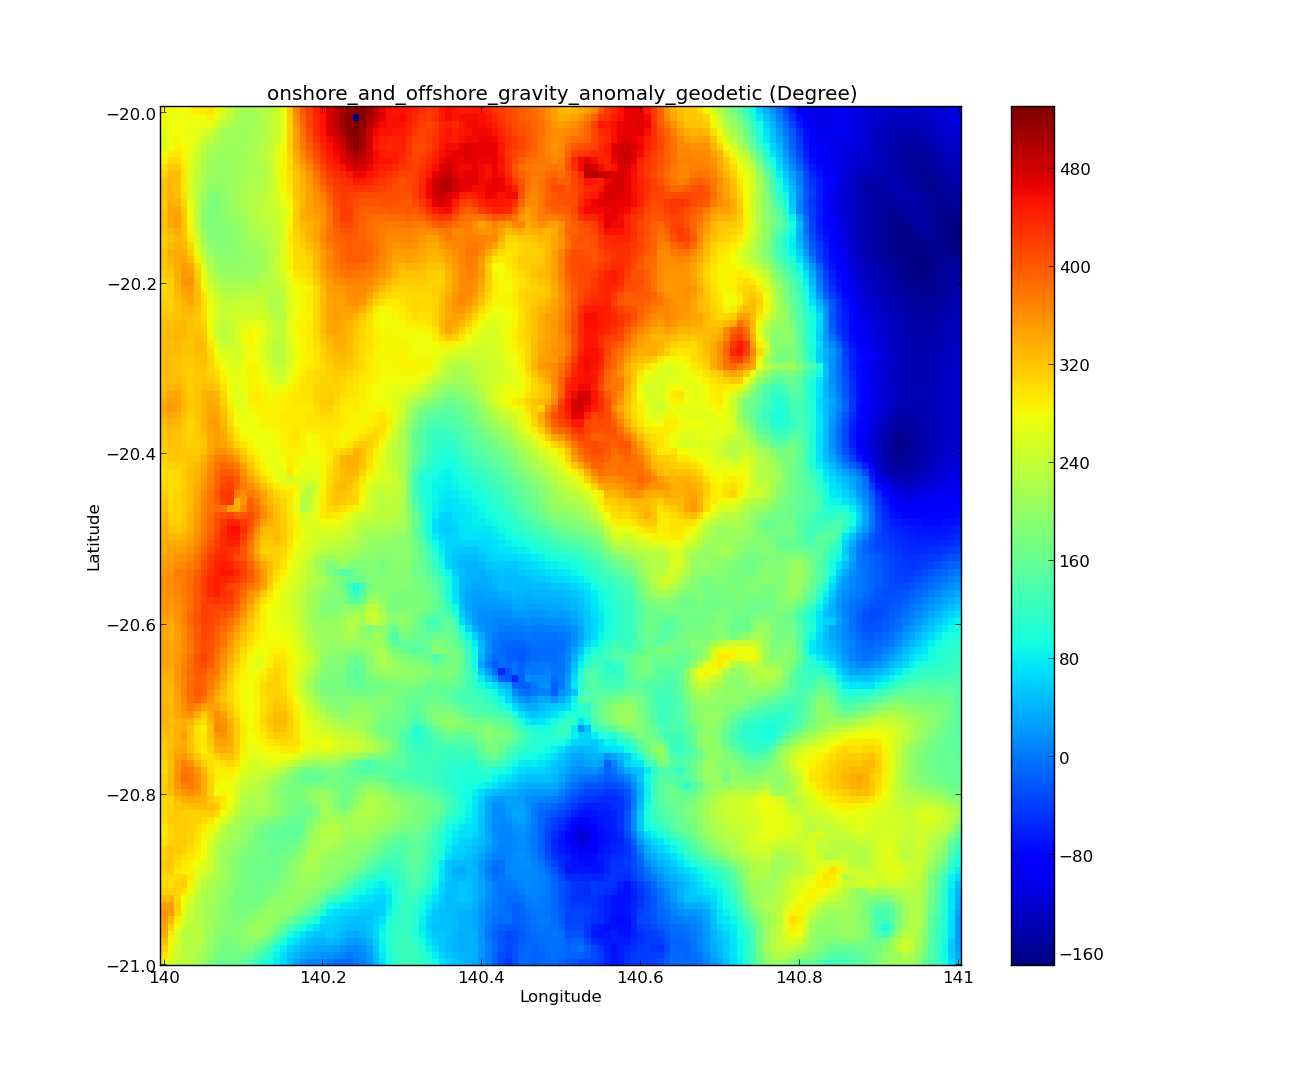
\includegraphics[width=0.7\textwidth]{QLDWestGravityDataPlot.png}
\caption{Gravity Anomaly Data in $mgal$ from Western Queensland, Australia
    (file \examplefile{data/QLDWestGravity.nc}). Data obtained from Geoscience Australia.}
%\AZADEH{Tracey R, Bacchin M, \& Wynne P. 2008. In preparation. AAGD07: A new absolute gravity datum for Australian gravity and new standards for the Australian National Gravity Database. Exploration Geophysics.}}
\label{FIG:P1:GRAV:0}
\end{figure}

\begin{figure}
\centering%
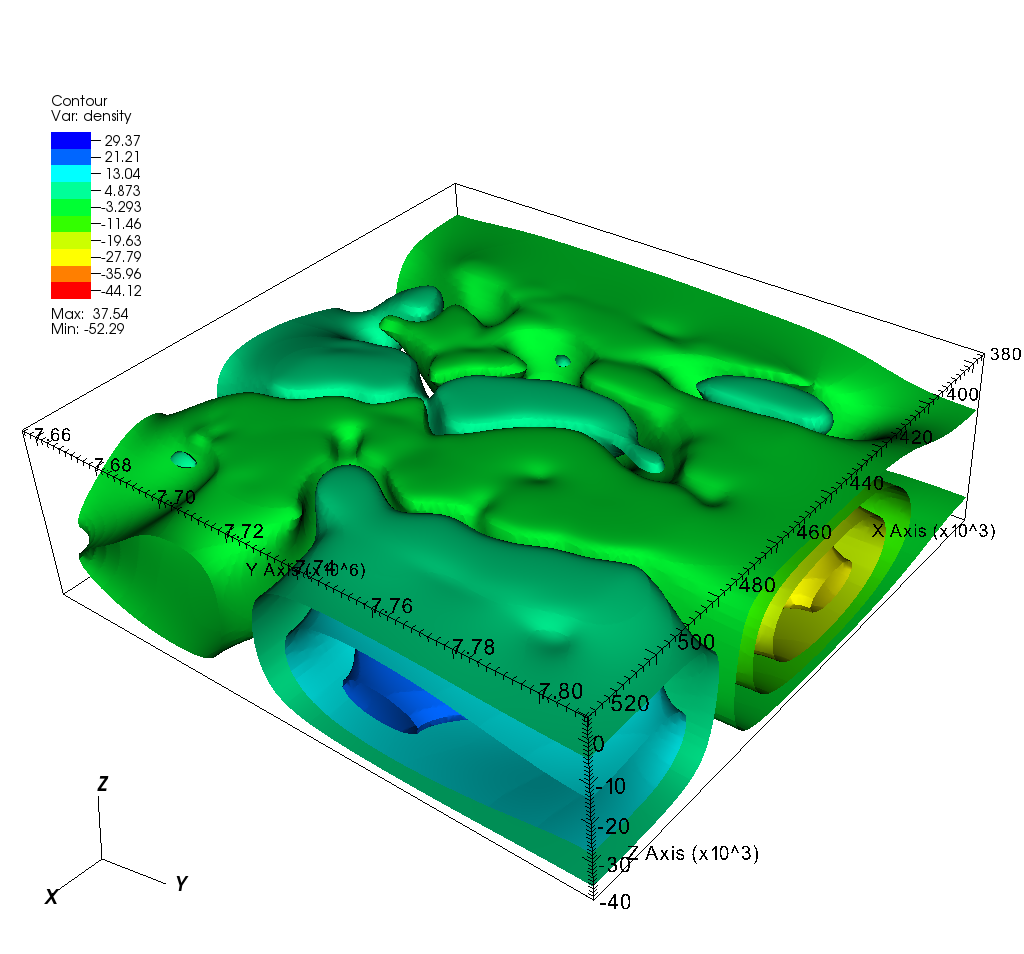
\includegraphics[width=0.9\textwidth]{QLDGravContourMu10.png}
\caption{3-D contour plot of the density distribution obtained by inversion of
    file \file{data/QLDWestGravity.nc} (with $\mu=10$).
    Colours represent values of density where high values are represented by
    blue and low values are represented by red.}
\label{FIG:P1:GRAV:1}
\end{figure}

\section{How does it work?}
The execution of the inversion is controlled by a script which, in essence, is
a text file and can be edited using any text editor.
The script contains a series of statements which are executed by an
interpreter which is an executable program reading the text file and executing
the statements line-by-line.
In the case of \downunder the interpreter is \Python.
In order to be able to process the statements in each line of the script
certain rules (called syntax) need to be obeyed.
There is a large number of online tutorials for \Python available\footnote{e.g.
\url{http://www.tutorialspoint.com/python} and \url{http://doc.pyschools.com}}.
We also refer to the \escript cook book \cite{ESCRIPTCOOKBOOK} and user's
guide \cite{ESCRIPT} which is in particular useful for users who like to dive
deeper into \downunder.
For this part of the manual no \Python knowledge is required but it is
recommended that users acquire some basic knowledge on \Python as they
progress in their work with \downunder.

The following script~\ref{code: gravity1}\footnote{The script is similar to
\examplefile{grav_netcdf.py} within the \escript example file directory.} is a
simple example to run an inversion for gravity data:

\begin{pyc}\label{code: gravity1}
\
\begin{python}
# Header:
from esys.downunder import *
from esys.weipa import *
from esys.escript import unitsSI as U

# Step 1: set up domain
dom=DomainBuilder()
dom.setVerticalExtents(depth=40.*U.km, air_layer=6.*U.km, num_cells=25)
dom.setFractionalPadding(pad_x=0.2, pad_y=0.2)
dom.fixDensityBelow(depth=40.*U.km)

# Step 2: read gravity data
source0=NetCdfData(NetCdfData.GRAVITY, 'GravitySmall.nc')
dom.addSource(source0)

# Step 3: set up inversion
inv=GravityInversion()
inv.setSolverTolerance(1e-4)
inv.setSolverMaxIterations(50)
inv.setup(dom)

# Step 4: run inversion 
inv.getCostFunction().setTradeOffFactorsModels(10.) 
rho = inv.run()

# Step 5: write reconstructed density to file
saveVTK("result.vtu", density=rho)
\end{python}
\end{pyc}
The result, in this case the density distribution, is written to an external
file for further processing. You can copy and paste the text of the script
into a file of any name, let's say for further reference we use the file
name \file{grav.py}.
It is recommended to use the extension \file{.py} to identify the file as a
\Python script.
We will discuss the statements of the script later in this chapter. 

Obviously the inversion needs to be fed with some gravity data. You can find
example data from western Queensland, Australia in two resolutions in the
\escript example directory. In this case the data are loaded from the file
\examplefile{GravitySmall.nc} which is given in the \netcdf file format.
After you have copied this file into the directory in which you have saved the
script \file{grav.py} you can run the program using the command line 
\begin{verbatim}
run-escript grav.py
\end{verbatim}
We are running \file{grav.py} through the \escript start-up command since
\escript is used as a back end for the inversion algorithm\footnote{Please see
the \escript user's guide~\cite{ESCRIPT} on how to run your script in parallel
using threading and/or MPI.}.
Obviously it is assumed that you have an installation of \escript available on
your computer, see \url{https://launchpad.net/escript-finley}.

After the execution has successfully completed you will find the result file
\file{result.vtu} in the directory from where you have started the execution
of the script.
The file has the \VTK format and can be imported easily into many
visualization tools.
One option is the \mayavi package which is available on most platforms.
You can invoke the the visualization using the commands
\begin{verbatim}
mayavi2 -d result.vtu -m SurfaceMap
\end{verbatim}
from the command line.
Figure~\ref{FIG:P1:GRAV:1} shows the result of this inversion as a contour
plot\footnote{These plots were generated by \VisIt using the higher resolution
data.}, while the gravity anomaly data is shown in Figure~\ref{FIG:P1:GRAV:0}.
We will discuss data later in Section~\ref{SEC:P1:GRAV:DATA}.

Let us take a closer look at the script\footnote{In \Python lines starting
with `\#` are comments and are not processed further.}. Besides the header
section one can separate the script into five steps:
\begin{enumerate}
    \item set up domain on which the inversion problem is solved
    \item load the data 
    \item set-up the inversion problem
    \item run the inversion
    \item further processing of the result. Here we write the reconstructed
          density distribution to a file.
\end{enumerate}
In the following we will discuss the steps of the scripts in more detail.
Before we do this it is pointed out that the header section, following
\Python conventions, makes all required packages available to access within
the script.
At this point we will not discuss this in more details but emphasize that the
header section is a vital part of the script.
It is is required in each \downunder inversion script and should not be
altered except if additional modules are needed.

\begin{figure}
\centering
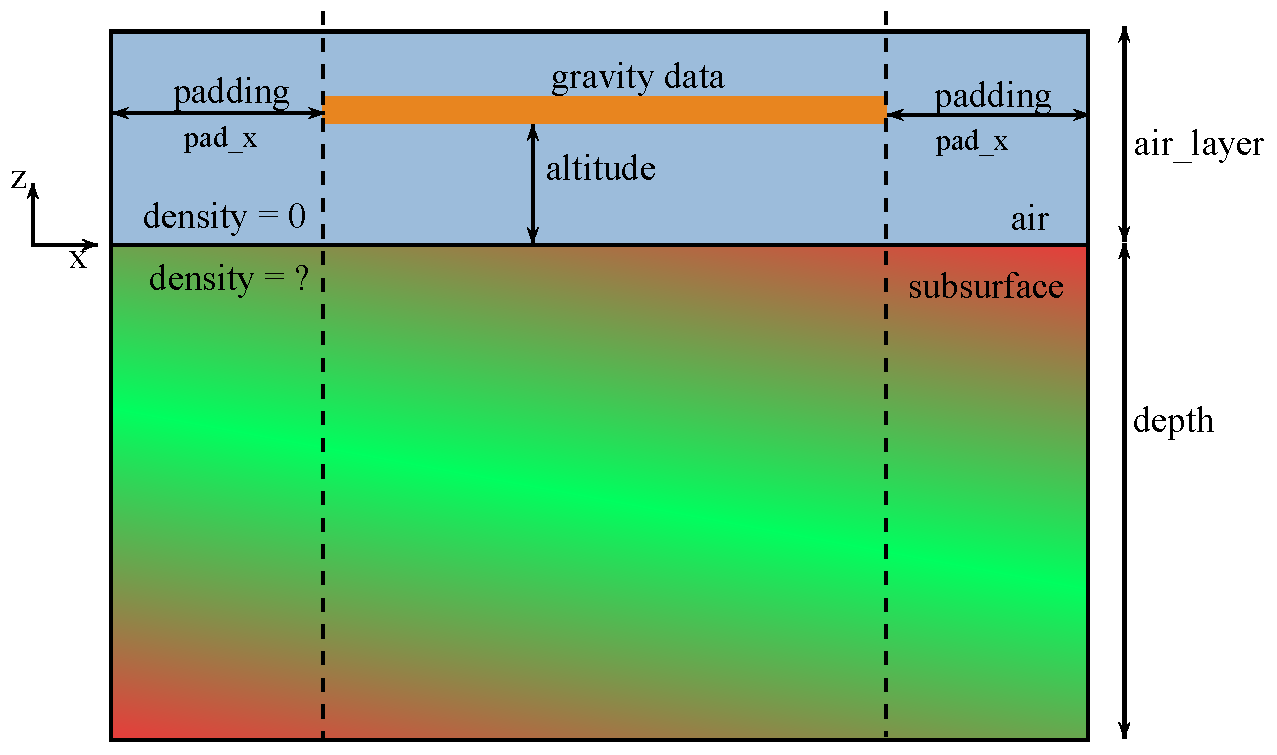
\includegraphics[width=\textwidth]{dom2D.pdf}
\caption{2-D domain set-up for gravity inversion}
\label{FIG:P1:GRAV:2}
\end{figure}

\section{Creating the Inversion Domain}
First step in Script~\ref{code: gravity1} is the definition of the domain over
which the inversion is performed.
We think of the domain as a block with orthogonal, plain faces.
Figure~\ref{FIG:P1:GRAV:2} shows the set-up for a two-dimensional domain
(see also Figure~\ref{fig:domainBuilder} for 3-D).
The lateral coordinates along the surface of the Earth are denoted by $x$ and
$y$ (only $x$-direction is used in 2-D).
The $z$ direction defines the vertical direction where the part above the
surface has positive coordinates and the subsurface negative coordinates.
The height of the section above the surface, which is assumed to be filled
with air, needs to be set by the user.
The inversion assumes that the density in the section is known to be
zero\footnote{Always keeping in mind that these are not absolute values but
anomalies.}.
The density below the surface is unknown and is calculated through the
inversion. The user needs to specify the depth below the surface in which the
density is to be calculated.
The lateral extension of the domain is defined by the data sets fed into the
inversion.
It is chosen large enough to cover all data sets (in case more than one is
used). In order to reduce the impact of the boundary a padding zone around the
data sets can be introduced.

\begin{figure}
\centering
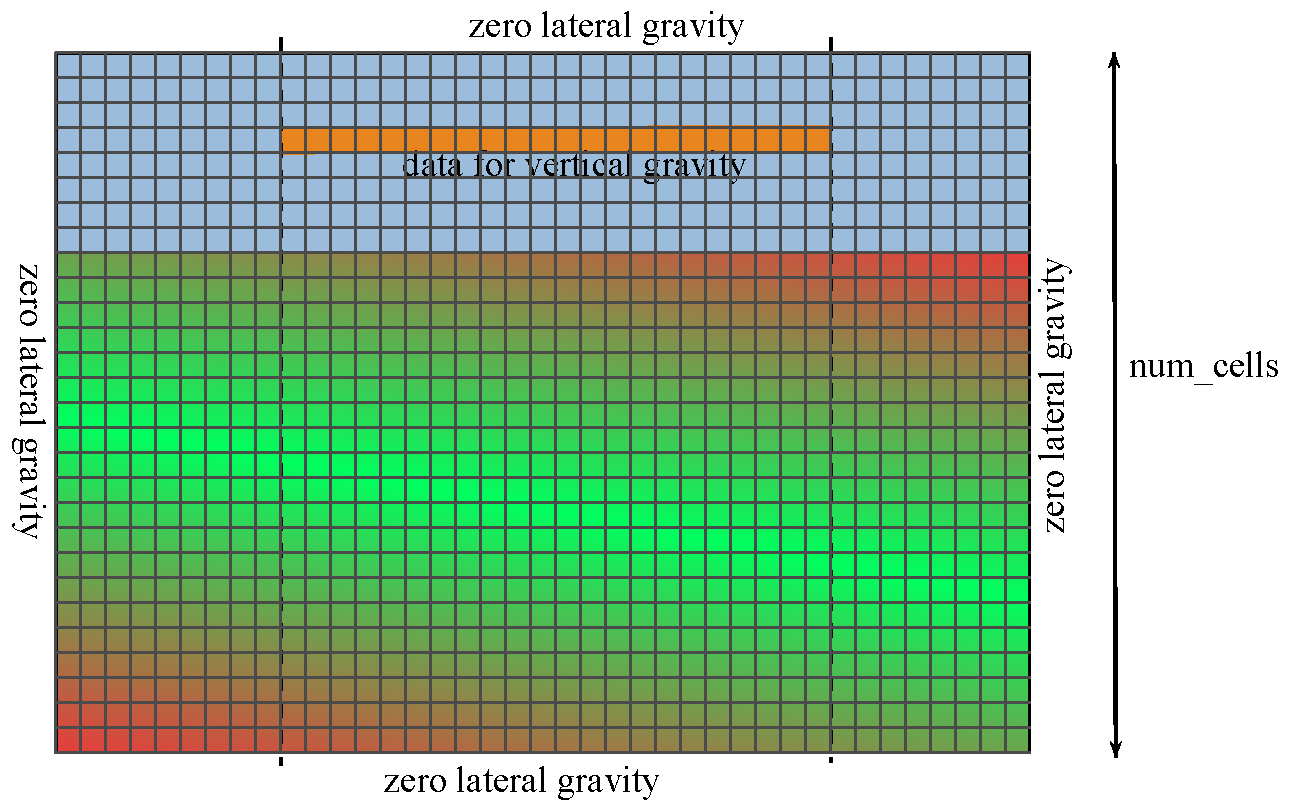
\includegraphics[width=\textwidth]{dom2DFEM.pdf}
\caption{Cell distribution and boundary conditions for a 2-D domain}
\label{FIG:P1:GRAV:3}
\end{figure}

The reconstruction of the gravity field from an estimated density distribution
is the key component of the inversion process.
To do this \downunder uses the finite element method (FEM).
We need to introduce a grid over the domain, see Figure~\ref{FIG:P1:GRAV:3}.
The number of vertical cells is set by the user while the number of horizontal
cells is derived from the grid spacing of the gravity data set(s).
It is assumed that gravity field data given are constant across a cell.
To be able to reconstruct the gravity field some assumptions on the values of
the gravity field on the domain boundary have to be made.
\downunder assumes that on all faces the lateral gravity field component
equals zero. No assumptions on the horizontal components are
made\footnote{It is assumed that the gravity potential equals zero on the top
and bottom surface, see Section~\ref{sec:forward gravity} for details}%
\footnote{Most inversion codes use Green's functions over an unbounded domain
to reconstruct the gravity field. This approach makes the assumption that the
gravity field (or potential) is converging to zero when moving away from the
region of interest. The boundary conditions used here are stronger in the
sense that the lateral gravity component is enforced to be zero in a defined
distance of the region of interest but weaker in the sense that no constraint
on the horizontal component is applied.}.
   
In script~\ref{code: gravity1} the statement
\begin{verbatim}
dom=DomainBuilder()
\end{verbatim}
creates something like a factory to build a domain.
We then define the features of the domain we would like to create:
\begin{verbatim}
dom.setVerticalExtents(depth=40.*U.km, air_layer=6.*U.km, num_cells=25)
dom.setFractionalPadding(pad_x=0.2, pad_y=0.2)
\end{verbatim}
Here we specify the depth of the domain to $40 km$, the thickness of the air
layer above the surface to $6 km$ and the number of vertical cells to $25$.
We also introduce a lateral padding of $20 \%$ of the expansion of the gravity
data on each side of the data and in both lateral directions.

In some cases it can be appropriate to assume that the density below a certain
depth is zero\footnote{As we are in fact calculating density corrections this
means that the density is assumed to be the average density.}.
The statement 
\begin{verbatim}
dom.fixDensityBelow(depth=40.*U.km)
\end{verbatim}
introduces this constraint.
As in the case discussed here if the depth for zero density is not less than
the depth of the domain no constraint at depth is applied to the density.

\downunder uses the metre-kilogram-second based International System of Units
(SI)\footnote{see \url{http://en.wikipedia.org/wiki/International_System_of_Units}}\index{SI}.
So all values must be converted to appropriate units.
This does not apply to geographic coordinates which in \downunder are given in
fractional degrees (as a floating point number) to represent longitude and
latitude. In the script we have used the expression
\begin{verbatim}
depth=40.*U.km
\end{verbatim}
to define the depth of the domain to $40 km$.
The expression \verb|U.km| denotes the unit $km$ (kilometer) and ensures
appropriate conversion of the value $40$ into the base unit $m$ (meter).
It is recommended to add units to values (where present) in order to make sure
that the final values handed into \downunder is given with the appropriate
units.
The physical units module of \escript, which we have imported here under the
name \verb|U| in the script header, defines a large number of physical units
and constants, please see~\cite{ESCRIPT} and~\cite{ESCRIPTONLINE}. 

\section{Loading Gravitational Data}\label{SEC:P1:GRAV:DATA}
In practice gravity acceleration is measured in various ways, for instance by
airborne surveys~\cite{Telford1990a}.
\downunder assumes that all data supplied as input are already appropriately
pre-processed. In particular, corrections for
\begin{itemize}
 \item free-air, to remove effects from altitude above ground;
 \item latitude, to remove effects from ellipsoidicity of the Earth;
 \item terrain, to remove effects from topography
\end{itemize}
must have been applied to the data.
In general, data prepared in such a form are called Bouguer anomalies~\cite{Telford1990a}.

To load gravity data into \downunder the data are given on a plane parallel
to the surface of the Earth at a constant altitude, see
diagram~\ref{FIG:P1:GRAV:2}.
The data need to be defined over a rectangular grid covering a subregion of
the Earth surface.
The grid uses a geographic coordinate system with latitudes and longitudes
assumed to be given in the Clarke 1866 geodetic system.
Figure~\ref{FIG:P1:GRAV:0} shows an example of such a data set from the
western parts of Queensland, Australia.
The data set covers a rectangular region between $140^o$ and $141^o$ east
and between $20^o$ and $21^o$ south.
Notice that latitude varies between $-90^o$ to $90^o$ where negative signs
refer to places in the southern hemisphere and longitude varies between
$-180^o$ to $180^o$ where negative signs refer to places west of Greenwich.
The colour at a location represents the value of the vertical Bouguer gravity
anomaly at this point at the surface of the Earth.
Values in this data set range from $-160 \; mgal$ to about $500 \; mgal$\footnote{The unit
$mgal$ means milli $gal$ (galileo) with $1 \; gal = 0.01 \frac{m}{sec^2}$.}
over a $121 \times 121$ grid.

In general, a patch of gravity data needs to be defined over a plane
\verb|NX| $\times$ \verb|NY| where \verb|NX| and \verb|NY| define the number
of grid lines in the longitude (\verb|X|) and the latitude (\verb|Y|)
direction, respectively.
The grid is spanned from an origin with spacing \verb|DELTA_X| and
\verb|DELTA_Y| in the longitude and the latitude direction, respectively.
The gravity data for all grid points need to be given as an \verb|NX|
$\times$ \verb|NY| array.
If available, measurement errors can be associated with the gravity data.
The values are given as an \verb|NX| $\times$ \verb|NY| array matching the
shape of the gravity array.
Note that data need not be available on every single point of the grid, see
Section~\ref{SEC:P1:GRAV:REMARK:DATAHOLES} for more information on this.

Currently, two data file formats are supported, namely \emph{ER Mapper Raster}
\cite{ERMAPPER} files and \netcdf~\cite{NETCDF} files.
In the examples of this chapter we use \netcdf files and refer to
Section~\ref{SEC:P1:GRAV:REMARK:ERMAPPER} and
Section~\ref{sec:ref:DataSource:ERM} for more information on using ER Mapper
Raster files.
If you have data in any other format you have the option of writing a suitable
reader (for advanced users, see Chapter~\ref{Chp:ref:data sources}) or,
assuming you are able to read the data in \Python, refer to the example
script \examplefile{create_netcdf.py} which shows how to create a file
in the \netcdf file format~\cite{NETCDF} compatible with \downunder from
a data array.

In script~\ref{code: gravity1} we use the statement 
\begin{verbatim}
source0=NetCdfData(NetCdfData.GRAVITY, 'GravitySmall.nc')
\end{verbatim}
to load the gravity data stored in \examplefile{GravitySmall.nc} in the
\netcdf format. 
Within the script the data set is now available under the name \verb|source0|.
We need to link the data set to the \verb|DomainBuilder| using 
\begin{verbatim}
dom.addSource(source0)
\end{verbatim}
At the time the domain for the inversion is built the \verb|DomainBuilder|
will use the information about origin, extent and spacing along with the other
options provided to build an appropriate domain.
As at this point a flat Earth is assumed geographic coordinates used to
represent data in the input file are mapped to a (local) Cartesian coordinate
system. This is achieved by projecting the geographic coordinates into the
\emph{Universal Transverse Mercator} (UTM) coordinate system\footnote{See e.g.
\url{http://en.wikipedia.org/wiki/Universal_Transverse_Mercator_coordinate_system}}.

It is possible to add several, possibly overlapping data sets to the same
domain:
\begin{verbatim}
source0=NetCdfData(NetCdfData.GRAVITY, 'data0.nc')
source1=NetCdfData(NetCdfData.GRAVITY, 'data1.nc')
dom.addSource(source0)
dom.addSource(source1)
\end{verbatim}
However, due to the coordinate transformation all data sets must be located in
the same UTM zone. If a single dataset crosses UTM zones only the zone of the
central longitude is used when projecting.
For example, if one data set lies mostly in zone 51 but contains areas of zone
52, it is transformed using zone 51.
In this case more data from zone 51 can be added, but not from any other zone.

There are a few optional arguments you can add when constructing a data source.
While Section~\ref{sec:ref:DataSource} has a detailed description of all
arguments it is worth noting a few.
Firstly, it is important to know that data slices are assumed to be at altitude
$0$ by default. This can be easily changed though:
\begin{verbatim}
source0=NetCdfData(NetCdfData.GRAVITY, 'GravitySmall.nc', altitude=2.5*U.km)
\end{verbatim}
Another important setting is the scale or unit of the measurements.
The default is dependent on the data type and for gravity anomalies a scale
of $\frac{\mu m}{sec^2}$ (or $0.1 \; mgal$) is assumed.
To change the default scale to $mgal$ (which is $10^{-5} \frac{m}{sec^2}$),
you could use:
\begin{verbatim}
source0=NetCdfData(NetCdfData.GRAVITY, 'GravitySmall.nc', scale_factor=1e-5)
\end{verbatim}
Finally, it is possible to specify measurement errors (i.e. uncertainties)
alongside the data.
Since these can never be zero, a value of $2$ units is used if nothing else
has been specified.
The error value is assumed to be given in the same units as the data so the
default value translates to an error of $0.2 \; mgal$.
There are two possibilities to specify the error, namely by providing a
constant value which is applied to all data points:
\begin{verbatim}
source0=NetCdfData(NetCdfData.GRAVITY, 'GravitySmall.nc', error=1.7)
\end{verbatim}
or, if the information is available in the same \netcdf file under the name
\verb|errors|, provide \downunder with the variable name:
\begin{verbatim}
source0=NetCdfData(NetCdfData.GRAVITY, 'GravitySmall.nc', error="errors")
\end{verbatim}

It is important to keep an eye on the complexity of the inversion.
A good measure is the total number of cells being used.
Assume we have given a data set on a $20 \times 20$ grid and we add lateral
padding of, say, $20 \%$ to each side of the data, the lateral number of cells
becomes $(20\cdot 1.4)\times (20\cdot 1.4)=1.4^2\cdot 20^2\approx 2\cdot 10^2=800$.
If we use $20$ cells in the vertical direction we end up with a total number
of $800 \times 20 = 16,000$ cells.
This size can be easily handled by a modern desktop PC.
If we increase the grid size of the data to $40 \times 40$ points and use $40$
cells in the vertical extent we get a total of $(2\cdot 40^2)\cdot 40=128,000$
cells, a problem size which is considerably larger but can still be handled by
a desktop computer.
Taking this one step further, if the amount of data is increased to
$200\times 200$ points and we use $200$ cells in the vertical extent the
domain will contain $16,000,000$ ($16$ million) cells.
This scenario requires a computer with enough memory and (a) fast processor(s)
to run the inversion.
This estimate of complexity growth applies to the case where the increase
of data grid size is driven by an increase of resolution where it is
recommended to increase the vertical resolution in synch with the lateral
resolution. Note that if more than one data set is used the target resolution
will be the resolution of the finest data set.
In other cases the expansion of the region of interest drives an increase of
data grid size and the increase of total number of cells is less dramatic as
the vertical number of cells can remain constant while keeping a balanced
resolution in vertical and lateral direction.

\section{Setting up the Inversion and Running it}
We are now at step three of script~\ref{code: gravity1} in which the actual
inversion is set up.
First we create an empty inversion under the name \verb|inv|:
\begin{verbatim}
inv=GravityInversion()
\end{verbatim}
As indicated by the name we can use \verb|inv| to perform an inversion of
gravity data\footnote{\verb|GravityInversion| is a driver with a simplified
interface which is provided for convenience. See Part~\ref{part2} for more
details on how to write inversion scripts with more general functionality, e.g.
constraints.}. The inversion is an iterative process which sequentially
calculates updates to the density distribution in an attempt to improve the
match of the gravity field produced by the density distribution with the data.
Termination of the iteration is controlled by the tolerance which is set by
the user:
\begin{verbatim}
inv.setSolverTolerance(1e-4)
\end{verbatim}
Here we set the tolerance to $10^{-4}$, i.e. the iteration is terminated if
the maximum density correction is less than or equal to $10^{-4}$ relative to
the maximum value of estimated density anomaly.
In case the iteration does not converge a maximum number of iteration steps is
set:
\begin{verbatim}
inv.setSolverMaxIterations(50)
\end{verbatim}
If the maximum number of iteration steps (here $50$) is reached the iteration
process is aborted and an error message is printed.
In this case you can try to rerun the inversion with a larger value for the
maximum number of iteration steps.
If even for a very large number of iteration steps no convergence is achieved,
it is very likely that the inversion has not been set up properly.

The statement 
\begin{verbatim}
inv.setup(dom)
\end{verbatim}
links the inversion with the domain and the data.
At this step -- as we are solving a gravity inversion problem -- only
gravitational data attached to the domain builder \verb|dom| are considered.
Internally a cost function $J$ is created which is minimized during the
inversion iteration.
It is a combination of a measure of the data misfit of the gravity field from
the given density distribution and a measure of the smoothness of the density
distribution.
The latter is often called the regularization term.
By default the gradient of density is used as the regularization term, see
also Section~\ref{SEC:P1:GRAV:REMARK:REG}.
Obviously, the result of the inversion is sensitive to the weighting between
the misfit and the regularization.
This trade-off factor $\mu$ for the misfit function is set by the following
statement:
\begin{verbatim}
inv.getCostFunction().setTradeOffFactorsModels(0.1) 
\end{verbatim}
Here we set $\mu=0.1$. The statement \verb|inv.setup| must appear in the
script before setting the trade-off factor.
A small value for the trade-off factor $\mu$ will give more emphasis to the
regularization component and create a smoother density distribution.
A large value of the trade-off factor $\mu$ will emphasize the misfit more
and typically creates a better fit to the data and a rougher density
distribution.
It is important to keep in mind that the regularization reduces noise in the
date and in fact gives the problem a unique solution.
Consequently, the trade-off factor $\mu$ may not be chosen too large in order
control the noise on the solution and ensure convergence in the iteration
process.

We can now actually run the inversion:
\begin{verbatim}
rho = inv.run()
\end{verbatim}
The answer as calculated during the inversion is returned and can be accessed
under the name \verb|rho|.
As pointed out earlier the iteration process may fail in which case the
execution of the script is aborted with an error message.

\section{Taking a Look}
In the final step of script~\ref{code: gravity1} the calculated density
distribution is written to an external file.
A popular file format used by several visualization packages such as
\VisIt~\cite{VISIT} and \mayavi~\cite{MAYAVI} is the \VTK file format.
The result of the inversion which has been named \verb|rho| can be written to
the file \file{result.vtu} by adding the statement
\begin{verbatim}
saveVTK("result.vtu", density=rho)
\end{verbatim}
at the end of script.
The inversion solution is tagged with the name \verb|density| in the result
file, however any other name for the tag could be used.
As the format is text-based (as opposed to binary) \VTK files tend to be very
large and take compute time to create, in particular when it comes to large
numbers of cells ($>10^6$).
For large problems it is more efficient to use the \SILO file format~\cite{SILO}.
\SILO files tend to be smaller and are faster generated and read.
It is the preferred format to import results into the visualization program
\VisIt~\cite{VISIT} which is particularly suited for the visualization of
large data sets.
Inversion results can directly exported into \SILO files using the statement
\begin{verbatim}
saveSilo("result.silo", density=rho)
\end{verbatim}
replacing the \verb|saveVTK(...)| statement.
Similar to \VTK files the result \verb|rho| is tagged with the name
\verb|density| so it can be identified in the visualization program.

\begin{figure}
    \begin{center}
        \subfigure[$\mu=0.1$]{%
            \label{FIG:P1:GRAV:10 MU01}
            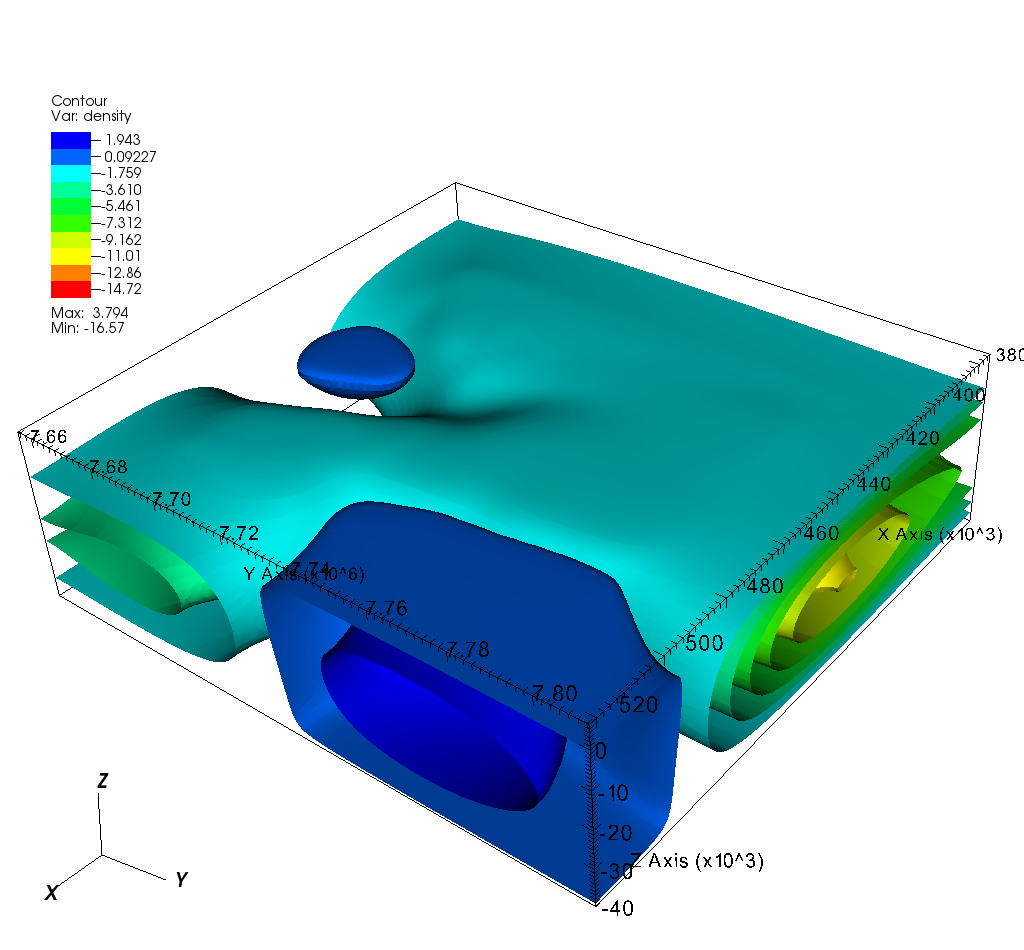
\includegraphics[width=0.45\textwidth]{QLDGravContourMu01.png}
        }%
        \subfigure[$\mu=1.$]{%
            \label{FIG:P1:GRAV:10 MU1}
            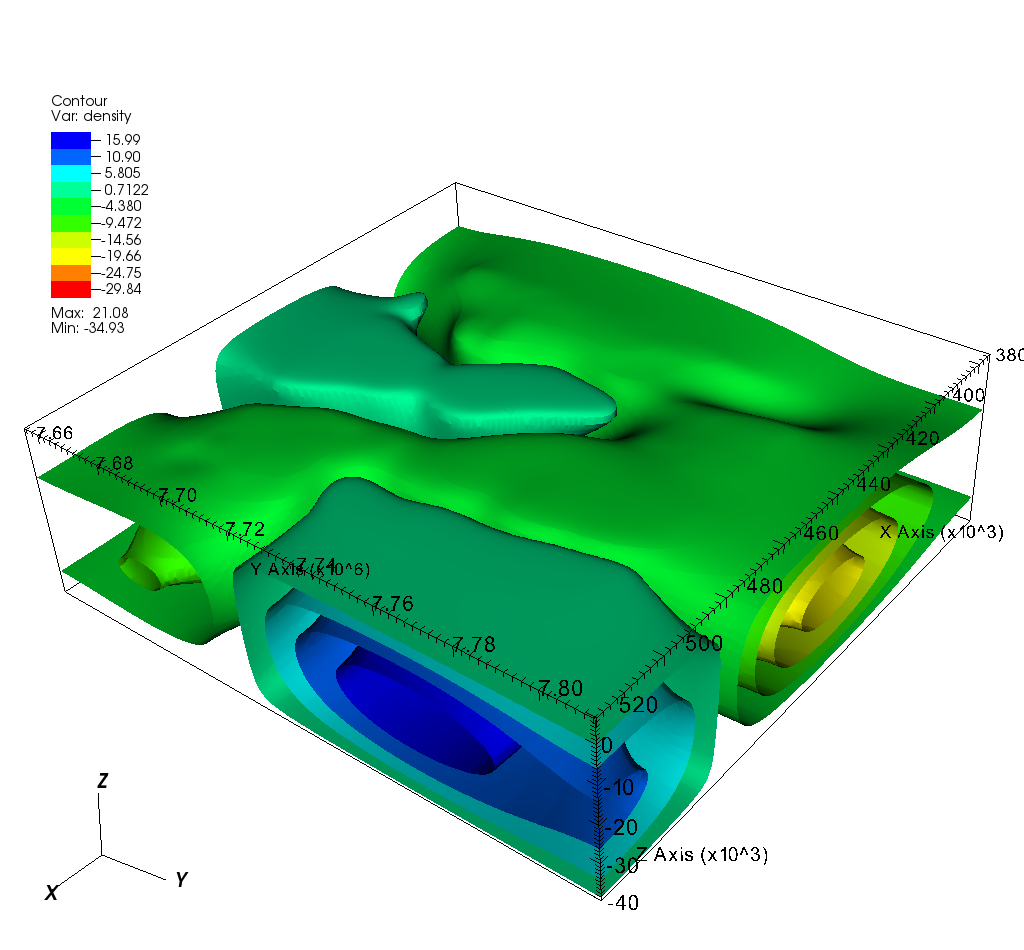
\includegraphics[width=0.45\textwidth]{QLDGravContourMu1.png}
        }\\ %  ------- End of the first row ----------------------%
        \subfigure[$\mu=10.$]{%
            \label{FIG:P1:GRAV:10 MU10}
            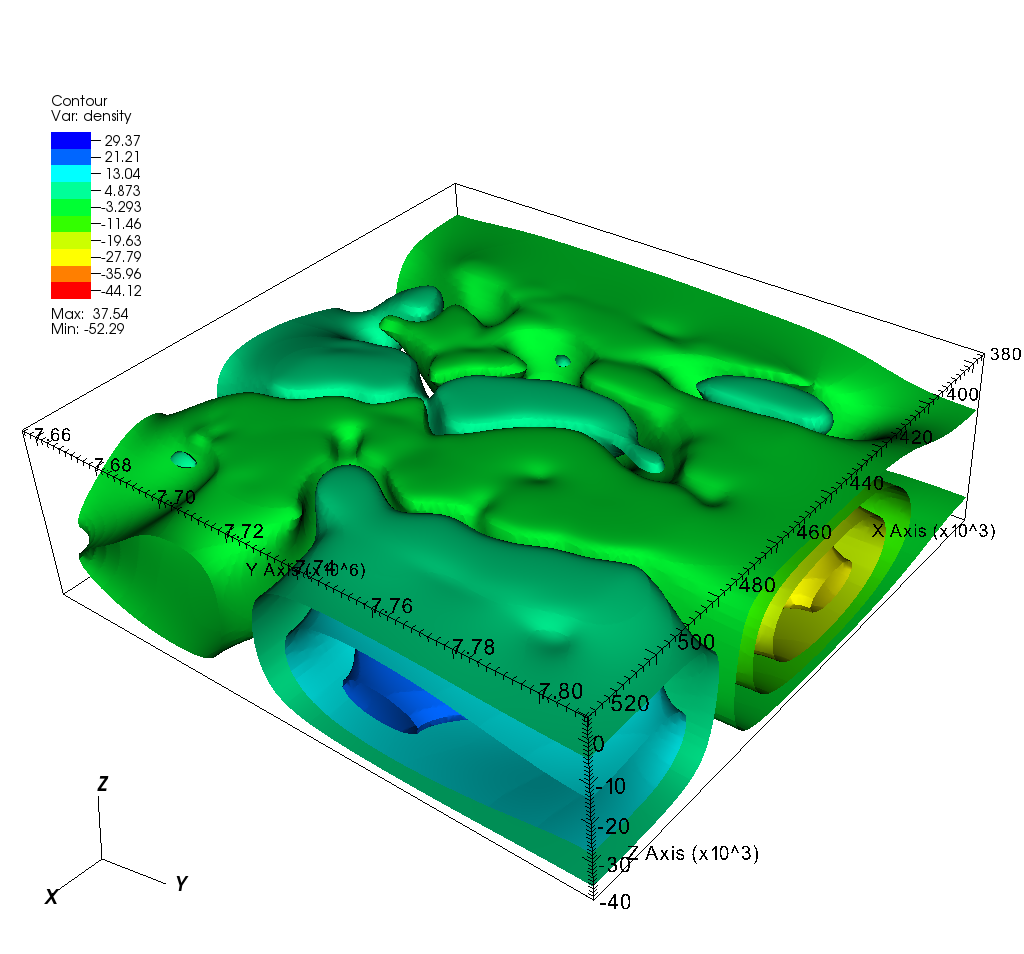
\includegraphics[width=0.45\textwidth]{QLDGravContourMu10.png}
        }%
        \subfigure[$\mu=100.$]{%
            \label{FIG:P1:GRAV:10 MU100}
            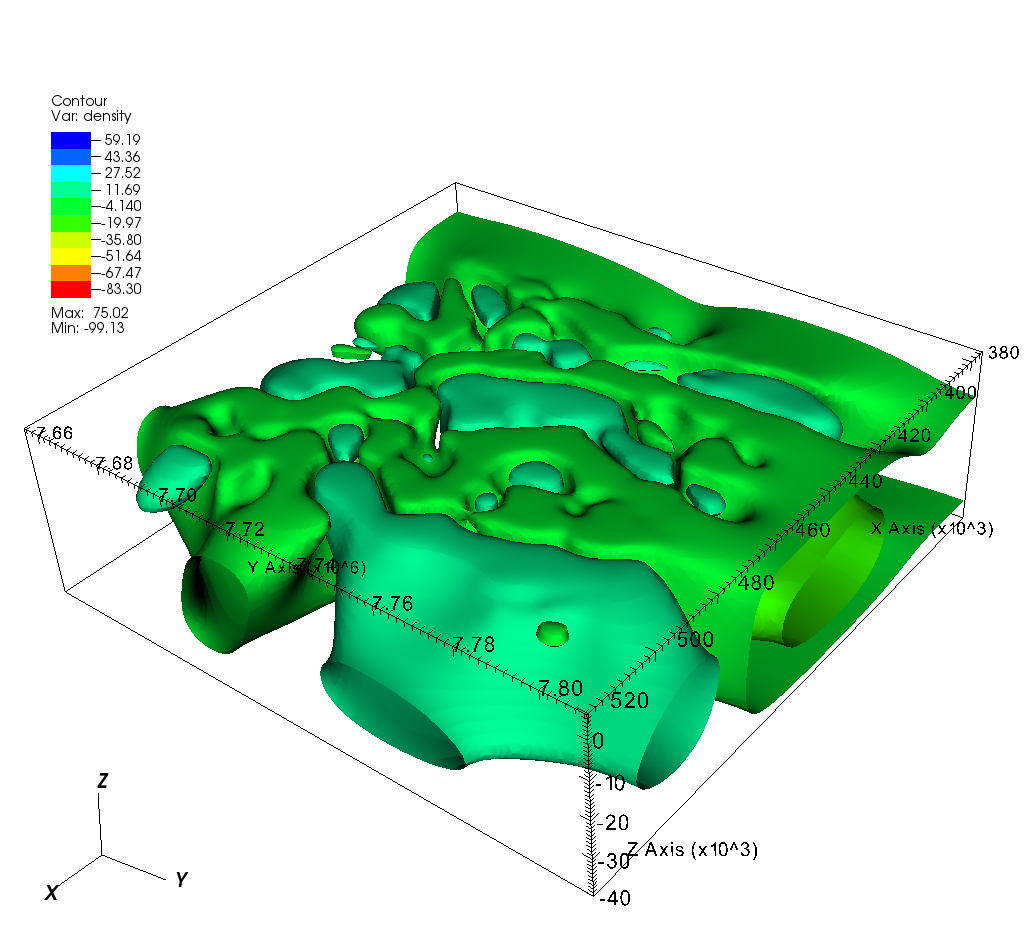
\includegraphics[width=0.45\textwidth]{QLDGravContourMu100.png}
        }\\ %  ------- End of the second row ----------------------%
        \subfigure[$\mu=1000.$]{%
            \label{FIG:P1:GRAV:10 MU1000}
            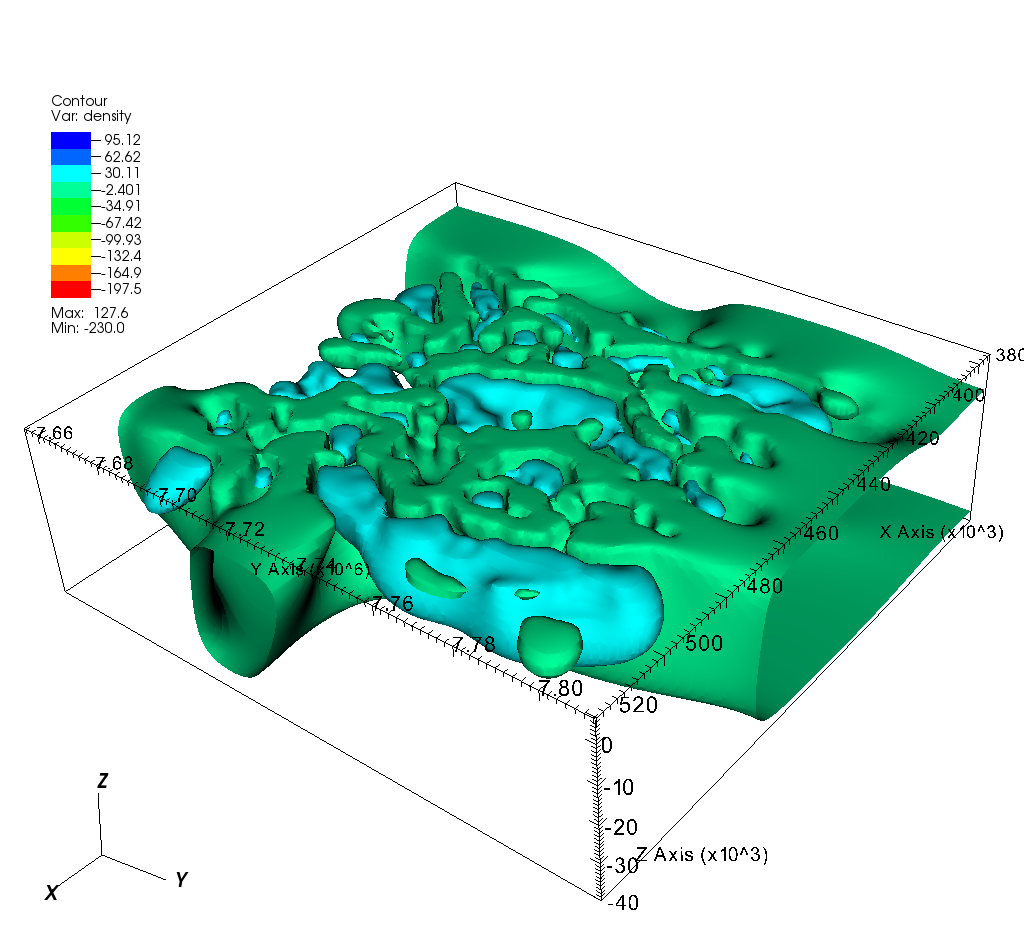
\includegraphics[width=0.45\textwidth]{QLDGravContourMu1000.png}
        }%
    \end{center}
    \caption{3-D contour plots of gravity inversion results with data from
    Figure~\ref{FIG:P1:GRAV:0} for various values of the model trade-off
    factor $\mu$. Visualization has been performed in \VisIt.
    \AZADEH{check images.}}
    \label{FIG:P1:GRAV:10}
\end{figure}

\begin{figure}
    \begin{center}
        \subfigure[$\mu=0.1$]{%
            \label{FIG:P1:GRAV:11 MU01}
            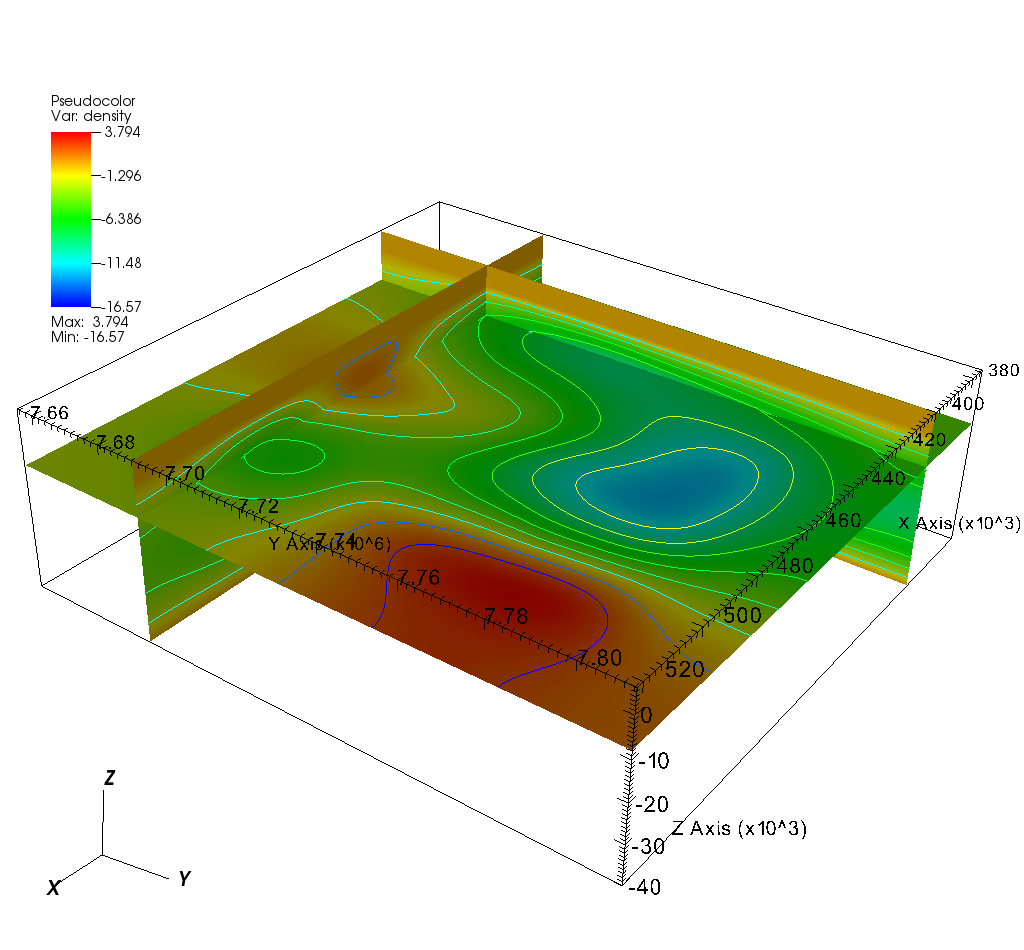
\includegraphics[width=0.45\textwidth]{QLDGravDepthMu01.png}
        }%
        \subfigure[$\mu=1.$]{%
            \label{FIG:P1:GRAV:11 MU1}
            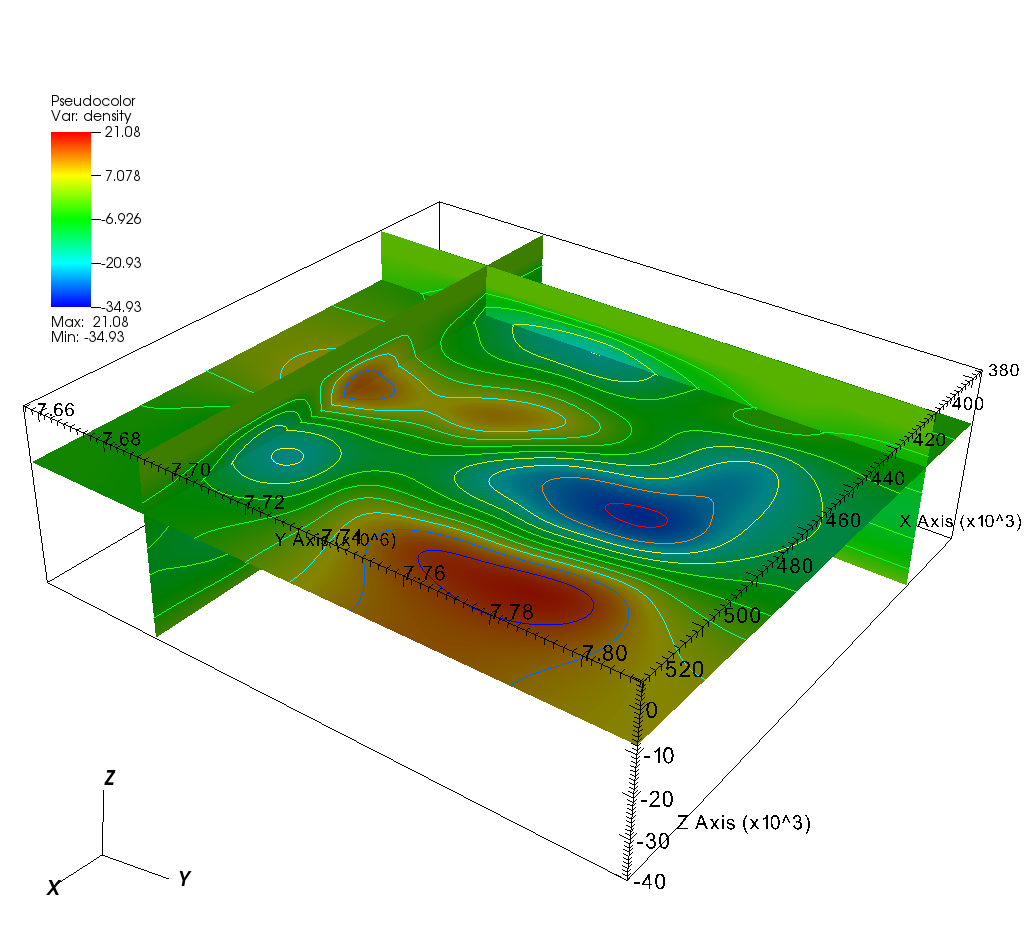
\includegraphics[width=0.45\textwidth]{QLDGravDepthMu1.png}
        }\\ %  ------- End of the first row ----------------------%
        \subfigure[$\mu=10.$]{%
            \label{FIG:P1:GRAV:11 MU10}
            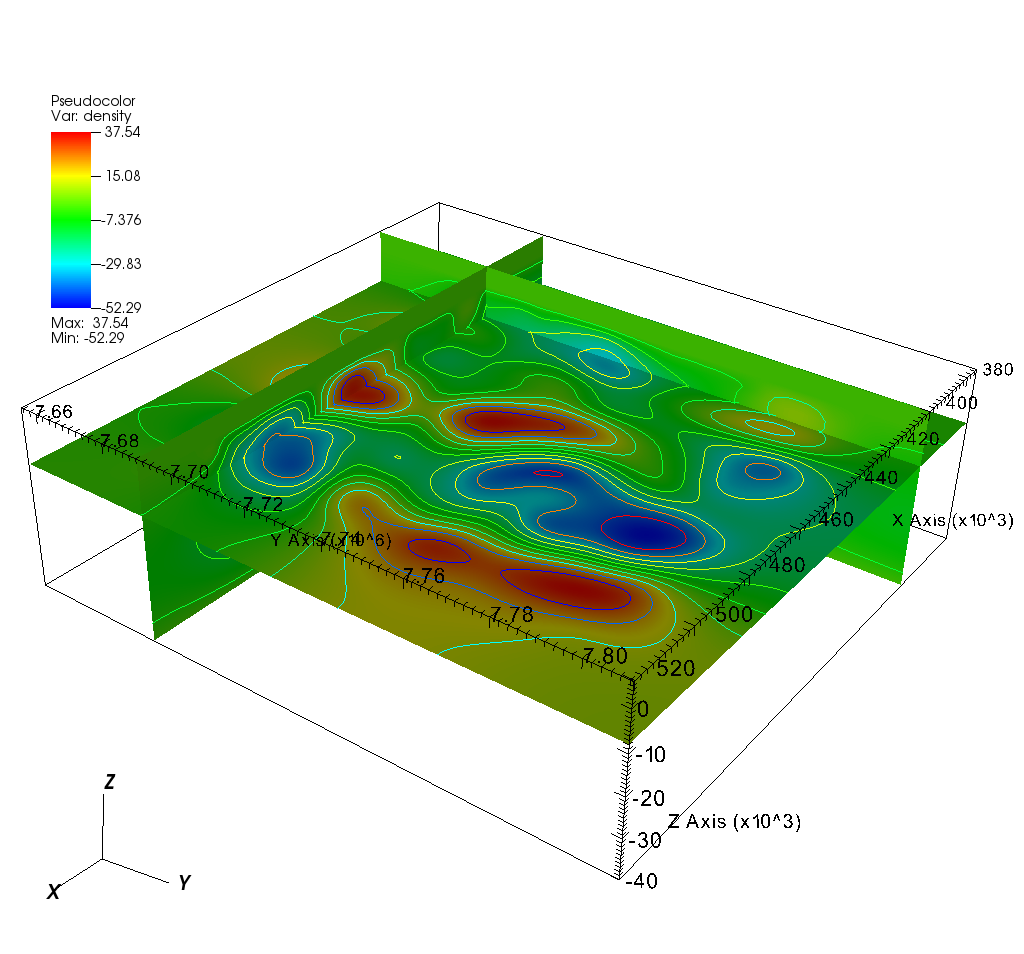
\includegraphics[width=0.45\textwidth]{QLDGravDepthMu10.png}
        }%
        \subfigure[$\mu=100.$]{%
            \label{FIG:P1:GRAV:11 MU100}
            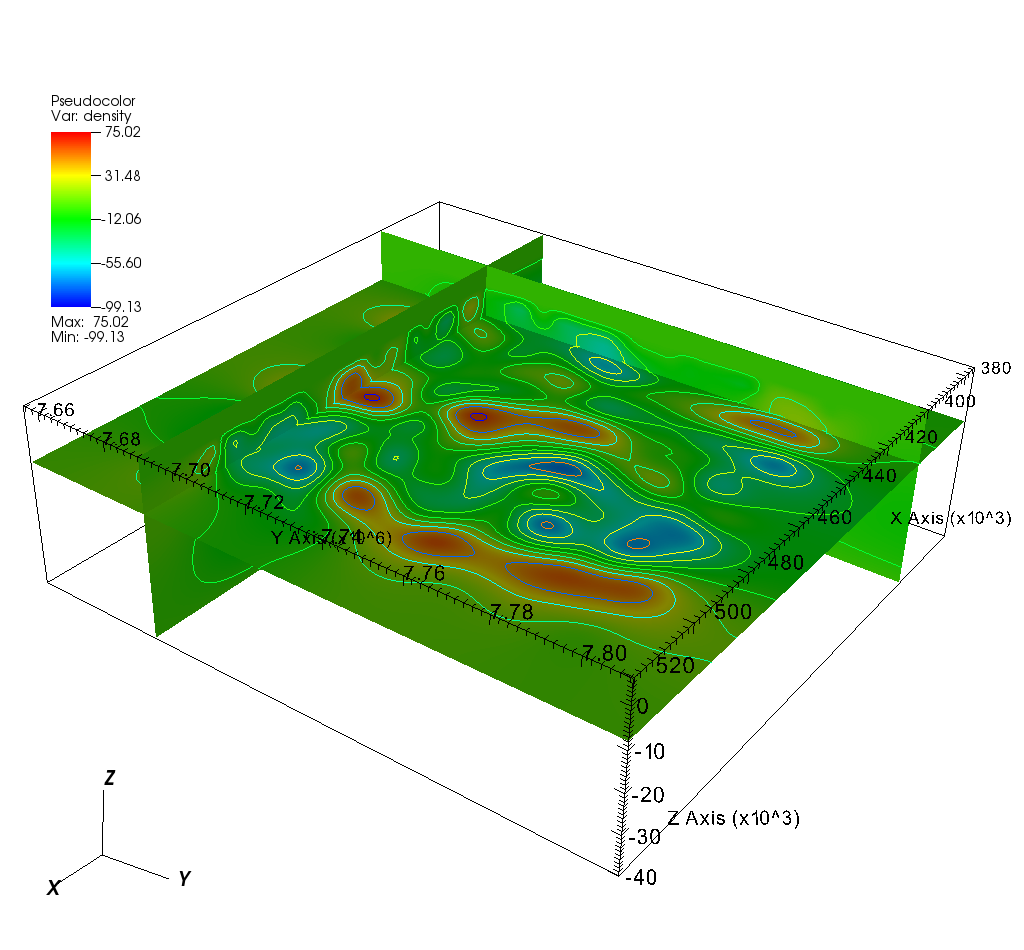
\includegraphics[width=0.45\textwidth]{QLDGravDepthMu100.png}
        }\\ %  ------- End of the second row ----------------------%
        \subfigure[$\mu=1000.$]{%
            \label{FIG:P1:GRAV:11 MU1000}
            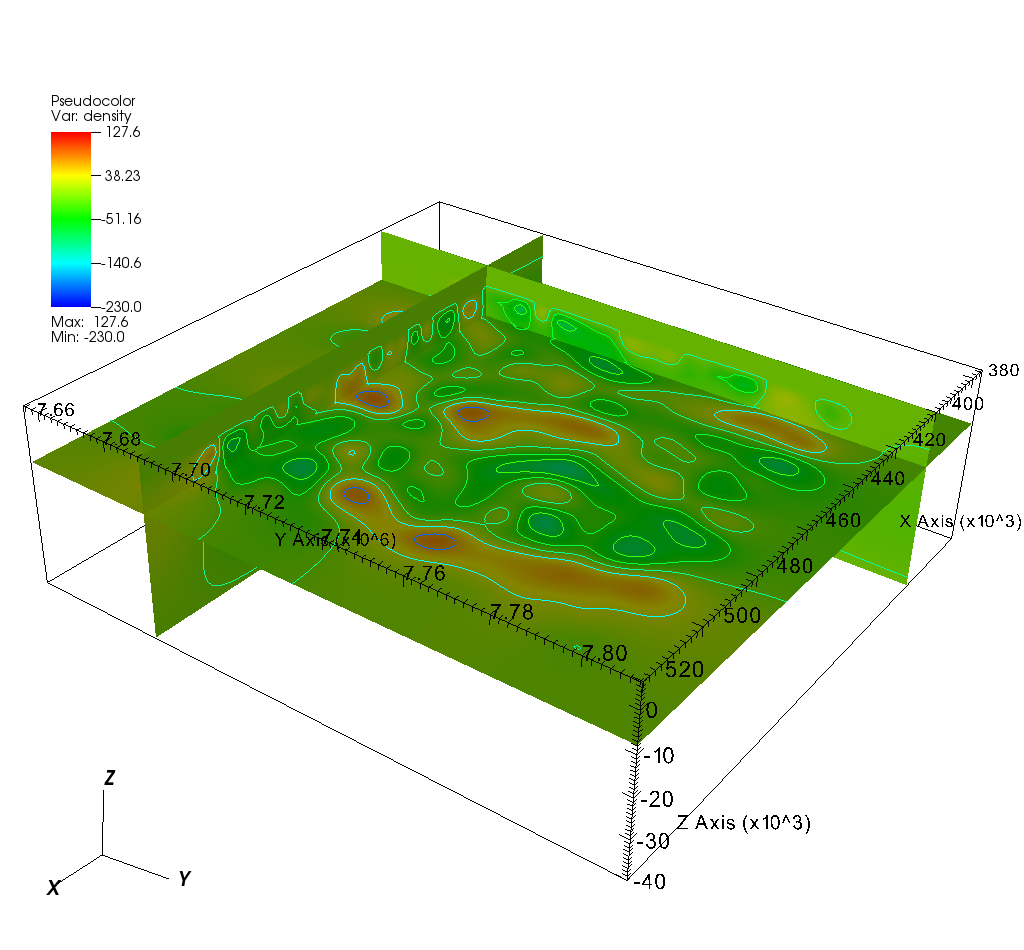
\includegraphics[width=0.45\textwidth]{QLDGravDepthMu1000.png}
        }%
    \end{center}
    \caption{3-D slice plots of gravity inversion results with data from
    Figure~\ref{FIG:P1:GRAV:0} for various values of the model trade-off
    factor $\mu$. Visualization has been performed \VisIt.
    \AZADEH{check images.}}
    \label{FIG:P1:GRAV:11}
\end{figure}

Figures~\ref{FIG:P1:GRAV:10} and~\ref{FIG:P1:GRAV:11} show two different
styles of visualization generated in \VisIt using the result of the inversion
of the gravity anomalies shown in Figure~\ref{FIG:P1:GRAV:0}.
The inversions have been performed with different values for the model
trade-off factor $\mu$.
The visualization shows clearly the smoothing effect of lower values for the
trade-off factors.
For larger values of the trade-off factor the density distribution becomes
rougher showing larger details.
Computational costs are significantly higher for larger trade-off factors.
Moreover, noise in the data has a higher impact on the result.
Typically several runs are required to adjust the value for the trade-off
factor to the datasets used.

For some analysis tools it is useful to process the results in form of
Comma-separated Values (\CSV)\footnote{see 
\url{http://en.wikipedia.org/wiki/Comma-separated_values}}.
Such a file can be created using the statement
\begin{verbatim}
saveDataCSV("result.csv", x=rho.getFunctionSpace().getX(), density=rho)
\end{verbatim}
in the script.
This will create a \file{result.csv} with columns separated by a comma.
Each row contains the value of the density distribution and the three
coordinates of the corresponding location in the domain.
There is a header specifying the meaning of the corresponding column.
Notice that rows are not written in a particular order and therefore, if
necessary, the user has to apply appropriate sorting of the rows.
Columns are written in alphabetic order of their corresponding tag names.
For the interested reader: the statement \verb|rho.getFunctionSpace()| returns
the type used to store the density data \verb|rho|.
The \verb|getX()| method returns the coordinates of the sampling points used
for the particular type of representation, see~\cite{ESCRIPT} for details. 

\section{Remarks}

\subsection{Data With Holes}\label{SEC:P1:GRAV:REMARK:DATAHOLES}
As described in the previous section input data is always given in the form of
a rectangular grid with constant cell size in each dimension.
However, there are cases when this is not necessarily the case.
Consider an onshore data set which includes parts of the offshore region as in
Figure~\ref{FIG:P1:GRAV:onshoreoffshore}.
The valid data in this example has a value range of about $-600$ to $600$ and
the inversion is to be run based on these values only, disregarding the
offshore region.
In order to achieve that, the offshore region is \emph{masked} by using a
constant value which is not found within the onshore area.
Figure~\ref{FIG:P1:GRAV:onshoreoffshore} clearly shows this masked area in
dark blue since a mask value of $-1000$ was used.

\begin{figure}[ht]
    \centering
    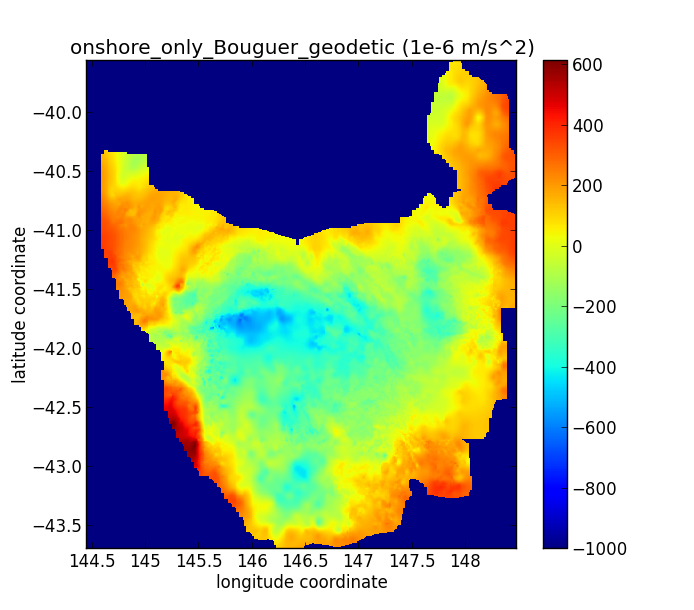
\includegraphics[width=0.45\textwidth]{onshore-offshore.png}
    \caption{Plot of a rectangular gridded onshore data set that includes
    offshore regions which have a value (here $-1000$) not found within the
    real data (Bouguer anomalies in Tasmania, courtesy Geoscience Australia)}
    \label{FIG:P1:GRAV:onshoreoffshore}
\end{figure}

The \netcdf conventions supported in \downunder include a standard way of
specifying such a mask value.
The example script \examplefile{create_netcdf.py} demonstrates how this is
accomplished in an easy way with any data.
If, for any reason, the mask value in the input file is invalid it can be
overridden via the \verb|null_value| argument when constructing the
\verb|NetCdfData| object:
\begin{verbatim}
source0=NetCdfData(NetCdfData.GRAVITY, 'data0.nc', null_value=-1000)
\end{verbatim}
In this example, all data points that have a value of $-1000$ are ignored and
not used in the inversion.
Please note that the special value \emph{NaN} (not-a-number) is sometimes used
for the purposes of masking in data sets.
Areas marked with this value are always disregarded in \downunder.

\subsection{ER Mapper Raster Files}\label{SEC:P1:GRAV:REMARK:ERMAPPER}
\CIHAN{ADD an example how to use ER Mapper raster files}

\subsection{Regularization Term}\label{SEC:P1:GRAV:REMARK:REG}
The \verb|GravityInversion| class supports the following form for the
regularization:
\begin{equation}
\int w^{(0)} \cdot \rho^2 + w^{(1)}_0  \rho_{,0}^2 +  w^{(1)}_1  \rho_{,1}^2 +  w^{(1)}_2  \rho_{,2}^2\; dx   
\end{equation}
where the integral is calculated across the entire domain.
$\rho$ represents the density distribution where $\rho_{,0}$ $\rho_{,1}$ and
$\rho_{,2}$ are the spatial derivatives of $\rho$ with respect to the two
lateral and the vertical direction, respectively.
$w^{(0)}$, $w^{(1)}_0$, $w^{(1)}_1$ and $w^{(1)}_2$ are weighting
factors\footnote{A more general form, e.g. spatially variable values for the
weighting factors, is supported, see Part~\ref{part2}}.
By default these are $w^{(0)}=0$, $w^{(1)}_0=w^{(1)}_1=w^{(1)}_2=1$.
Other weighting factors can be set in the inversion set-up.
For instance to set $w^{(0)}=10$, $w^{(1)}_0=w^{(1)}_1=0$ and $w^{(1)}_2=100$
use the statement:
\begin{verbatim}
inv.setup(dom, w0=10, w1=[0,0,100])
\end{verbatim}
It is pointed out that the weighting factors are rescaled in order to improve
numerical stability. Therefore the relative size of the weighting factors is
relevant and using
\begin{verbatim}
inv.setup(dom, w0=0.1, w1=[0,0,1])
\end{verbatim}
would lead to the same regularization as the statement above.

% 
% \section{Reference}
% 
% There are three examples for 2D and 3D gravity inversions with artificial input data.
% In first step, an area with synthetic density section was suggested. Then based on forward modeling its gravitational data was collected. Afterwards with generated gravity data, escripts simulated a volume of inverted density. Whilst new density mass could be compared with the synthetic density section to verify the inversion.
% 
% Some of the presumptions were the same for all of the examples to simplify the situation to make a logical comparison between synthetic input and output. which is as followed:
% 
% \begin{verbatim}
% n_cells_in_data=100
% depth_offset=0.*U.km
% l_data = 100 * U.km
% l_pad=40*U.km
% THICKNESS=20.*U.km
% l_air=6*U.km
% \end{verbatim}
% 
% The others assumptions comes with each examples.
% \begin{enumerate}
% \item  A 2D density section with a maximum in center was assumed. The reference density and inverted will be shown. The padding area is excluded. (\ref{fig:gravity2D1})
% 
% \begin{verbatim}
% n_cells_in_data=100
% n_humbs_h= 1
% n_humbs_v=1
% mu=100
% \end{verbatim}
% 
% \begin{figure}
% \centering
% 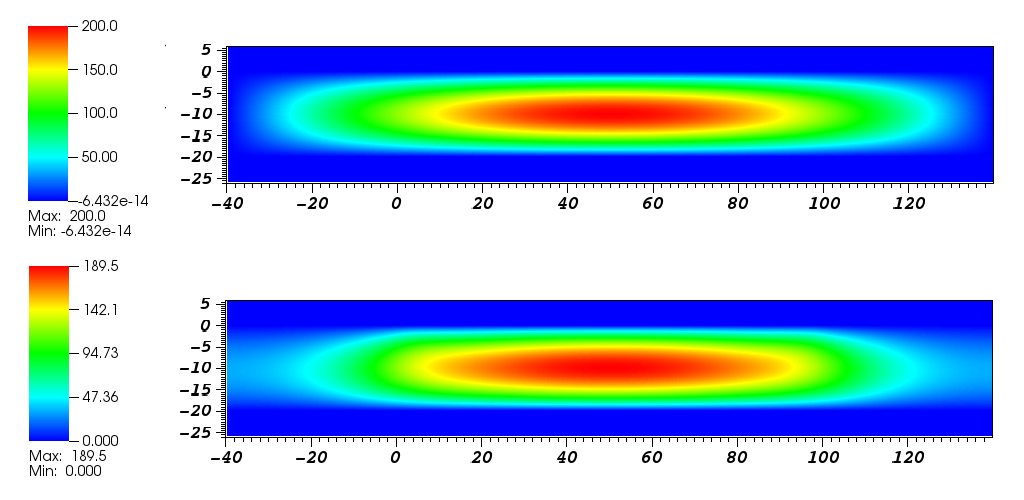
\includegraphics[width=\textwidth]{grav2D1.png}
% \caption{2D density model up) reference    down) result}
% \label{fig:gravity2D1}
% \end{figure}
% 
% 
% \item A 2D density properties with two maximum in corners and one minimum in the center was inverted. The result have eliminated the effects in padding area.(\ref{fig:gravity2D3}) 
% 
% \begin{verbatim}
% n_cells_in_data=100
% n_humbs_h= 3
% n_humbs_v=1
% mu=100
% \end{verbatim}
% 
% \begin{figure}
% \centering
% 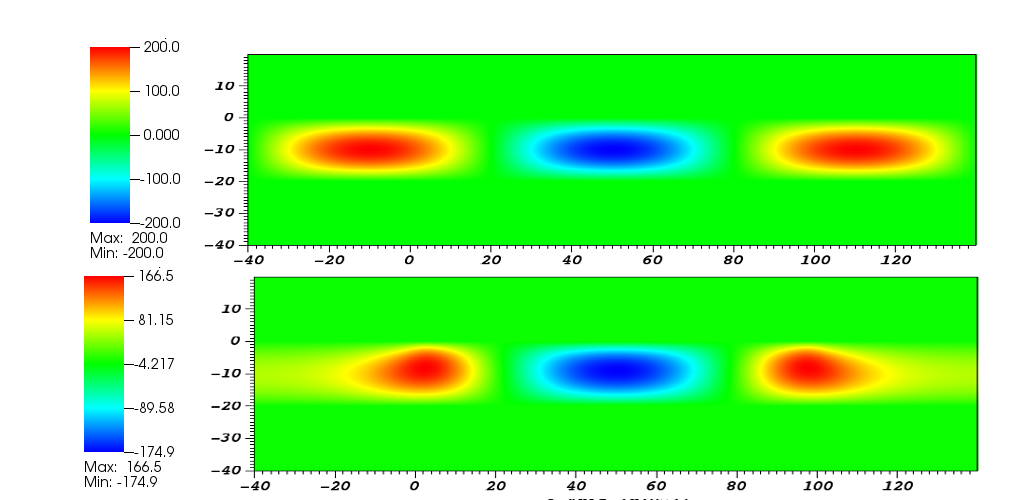
\includegraphics[width=\textwidth]{grav2D3.png}
% \caption{2D density model up) reference  down) result}
% \label{fig:gravity2D3}
% \end{figure}
% 
% \item A 3D model with a maximum in the center was used as input data and the result after simulation in shown in the next image which determined a good distribution of density through the model in the main area.(\ref{fig:gravity3D} and \ref{fig:gravity3D1})
% 
% \begin{verbatim}
% n_cells_in_data=50
% n_humbs_h= 1
% n_humbs_v=1
% mu=10
% \end{verbatim}
% 
% \begin{figure}
% \centering
% 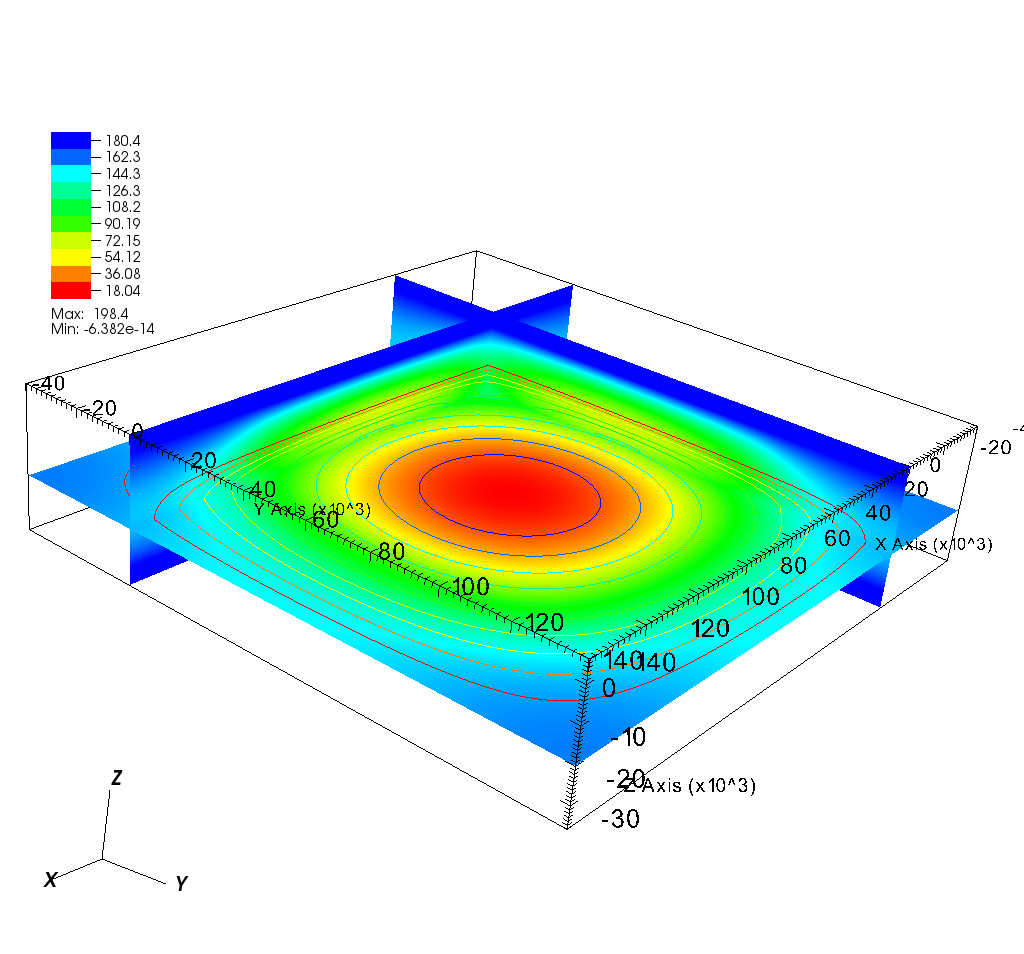
\includegraphics[width=\textwidth]{density3D-ref.png}
% \caption{3D density model of reference as synthetic data}
% \label{fig:gravity3D}
% \end{figure}
% 
% \begin{figure}
% \centering
% 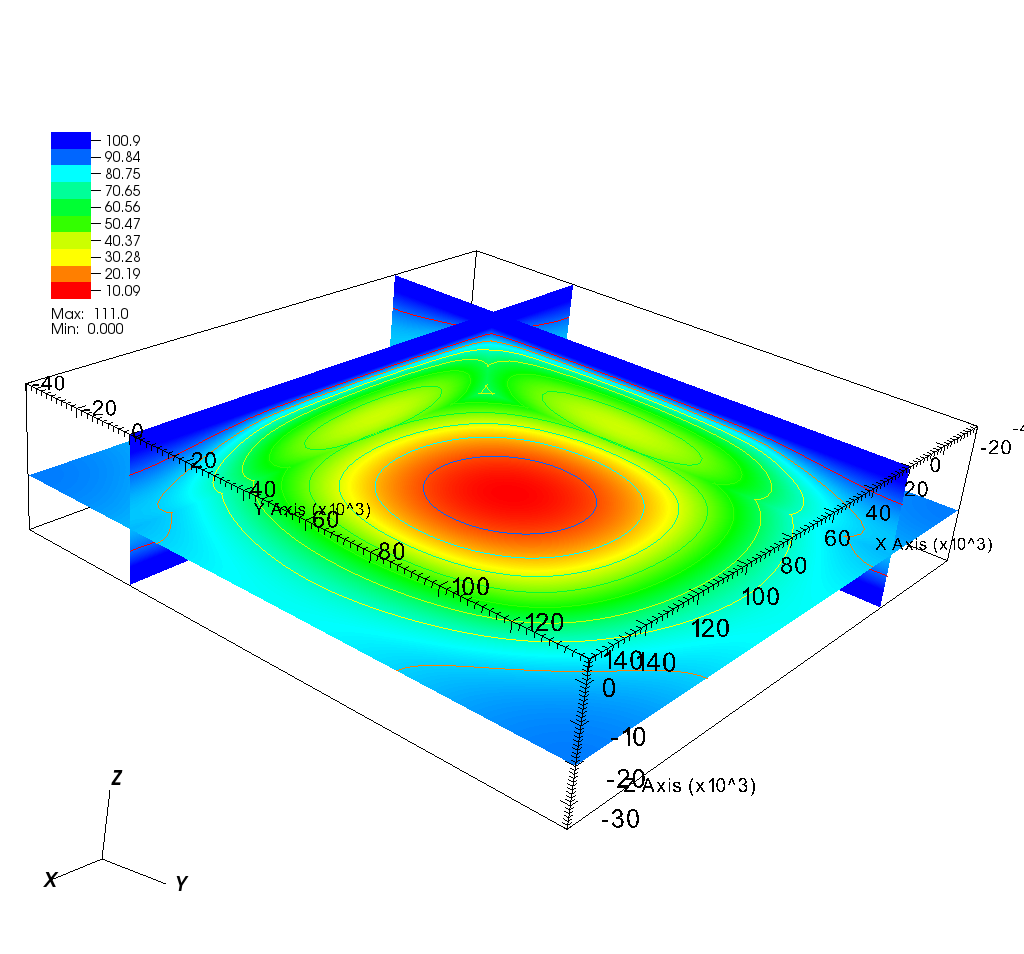
\includegraphics[width=\textwidth]{gravity3D.png}
% \caption{3D density model of result}
% \label{fig:gravity3D1}
% \end{figure}
% \end{enumerate}


\chapter{Magnetic Inversion}\label{Chp:cook:magnetic inversion}

\begin{figure}
\centering
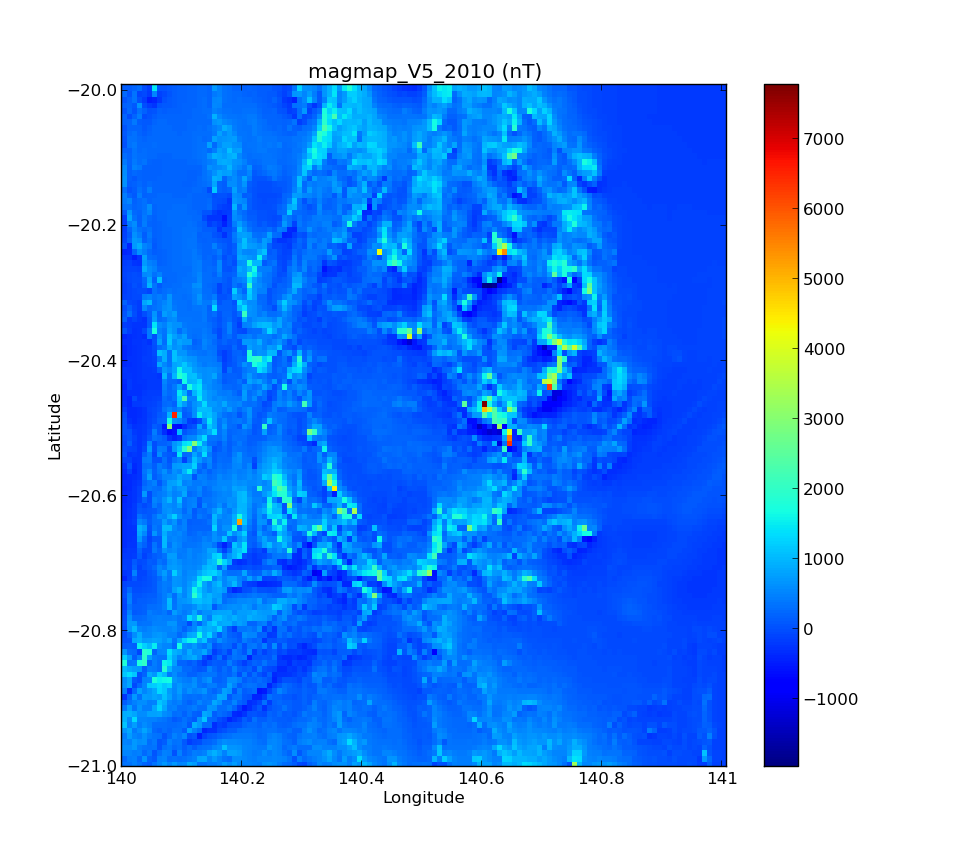
\includegraphics[width=0.7\textwidth]{QLDWestMagneticDataPlot.png}
\caption{Magnetic anomaly data in $nT$ from Western Queensland, Australia
    (file \examplefile{data/QLDWestMagnetic.nc}). Data obtained from Geoscience Australia.}
\label{FIG:P1:MAG:0}
\end{figure}

Magnetic data report the observed magnetic flux density over a region above the
surface of the Earth.
Similar to the gravity case the data are given as deviation from an expected
background magnetic flux density $B^b$ of the Earth.
Example data in units of $nT$ (nano Tesla) are shown in Figure~\ref{FIG:P1:MAG:0}.
It is the task of the inversion to recover the susceptibility distribution $k$
from the magnetic data collected. The approach for inverting magnetic data is
almost identical to the one used for gravity data. 
In fact the \downunder script~\ref{code: magnetic1} used for the magnetic
inversion is very similar to the script~\ref{code: gravity1} for gravity inversion.

\begin{pyc}\label{code: magnetic1}
\
\begin{python}
# Header:
from esys.downunder import *
from esys.weipa import *
from esys.escript import unitsSI as U


# Step 1: set up domain
dom=DomainBuilder()
dom.setVerticalExtents(depth=40.*U.km, air_layer=6.*U.km, num_cells=25)
dom.setFractionalPadding(pad_x=0.2, pad_y=0.2)
B_b = [31232.*U.Nano*U.Tesla, 2201.*U.Nano*U.Tesla, -41405.*U.Nano*U.Tesla]
dom.setBackgroundMagneticFluxDensity(B_b)
dom.fixSusceptibilityBelow(depth=40.*U.km)

# Step 2: read magnetic data
source0=NetCdfData(NetCdfData.MAGNETIC, 'MagneticSmall.nc', scale_factor=U.Nano * U.Tesla)
dom.addSource(source0)

# Step 3: set up inversion
inv=MagneticInversion()
inv.setSolverTolerance(1e-4)
inv.setSolverMaxIterations(50)
inv.fixMagneticPotentialAtBottom(False)
inv.setup(dom)

# Step 4: run inversion 
inv.getCostFunction().setTradeOffFactorsModels(0.1) 
k = inv.run()

# Step 5: write reconstructed susceptibility to file
saveVTK("result.vtu", susceptibility=k)
\end{python}
\end{pyc}

\begin{figure}
\centering
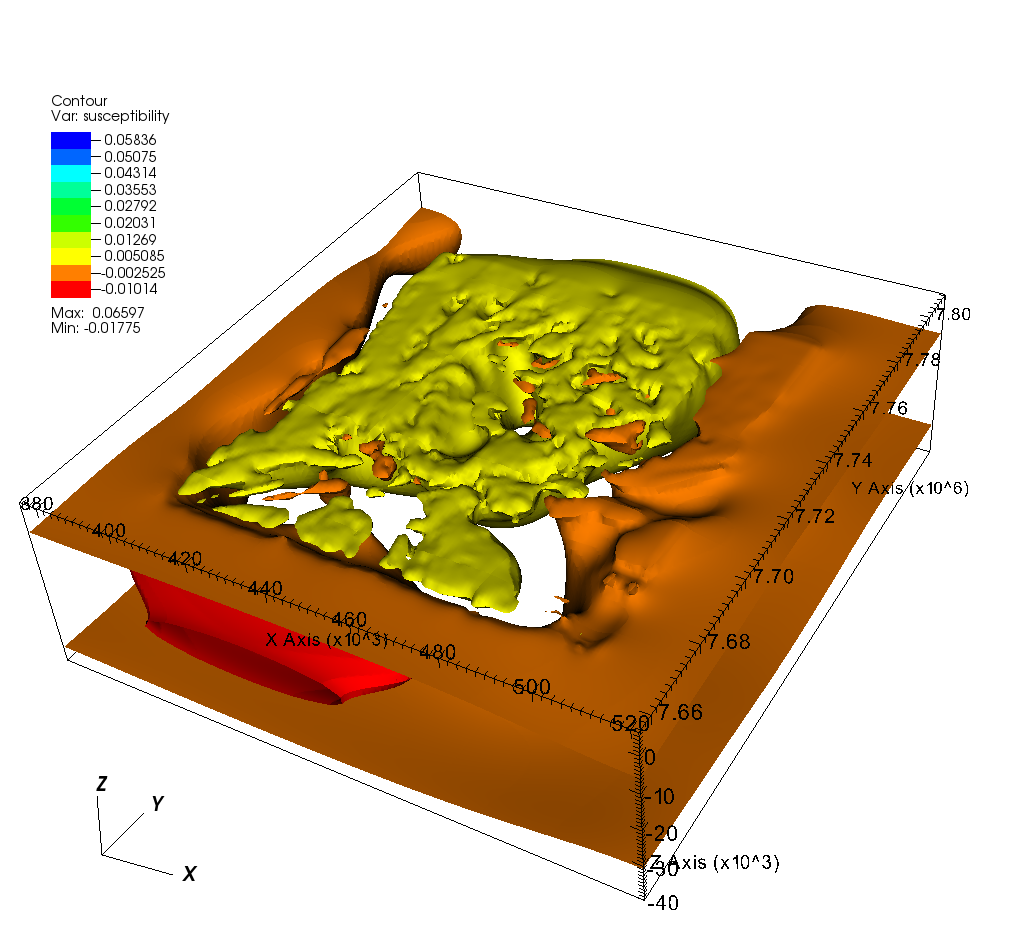
\includegraphics[width=0.7\textwidth]{QLDMagContourMu01.png}
\caption{Contour plot of the susceptibility from a three-dimensional magnetic inversion (with $\mu=0.1$).
Colours represent values of susceptibility where high values are represented by
    blue and low values are represented by red.}
\label{FIG:P1:MAG:1}
\end{figure}

The structure of the script is identical to the gravity case.
Following the header section importing the necessary modules the domain of the
inversion is defined in step one.
In step two the data are read and added to the domain builder.
Step three sets up the inversion and step four runs it.
Finally in step five the result is written to the result file, here
\file{result.vtu} in the \VTK format.
Results are shown in Figure~\ref{FIG:P1:MAG:1}.

Although scripts for magnetic and gravity inversion are largely identical there
are a few small differences which we are going to highlight now.
The magnetic inversion requires data about the background magnetic flux density
over the region of interest which is added to the domain by the statements 
\begin{verbatim}
B_b = [31232.*U.Nano*U.Tesla, 2201.*U.Nano*U.Tesla, -41405.*U.Nano*U.Tesla]
dom.setBackgroundMagneticFluxDensity(B_b)
\end{verbatim}
Here it is assumed that the background magnetic flux density is constant across
the domain and is given as the list
\begin{verbatim}
B_b= [ B_N,  B_E, B_V ]
\end{verbatim}
in units of Tesla (T) where 
\member{B_N}, \member{B_E} and \member{B_V} refer to the north, east and
vertical component of the magnetic flux density, respectively.
Values for the magnetic flux density can be obtained by the International
Geomagnetic Reference Field (IGRF)~\cite{IGRF} (or the Australian Geomagnetic
Reference Field (AGRF)~\cite{AGRF} via \url{http://www.ga.gov.au/oracle/geomag/agrfform.jsp}).
Similar to the gravity case susceptibility below a certain depth can be set to
zero via the statement
\begin{verbatim}
dom.fixSusceptibilityBelow(depth=40.*U.km)
\end{verbatim}
where here the susceptibility below $40km$ is prescribed (this has no effect as
the depth of the domain is $40km$)\footnote{Notice that the method called is
different from the one in the case of gravity inversion.}. 

Magnetic data are read and added to the domain with the following statements:
\begin{verbatim}
source0=NetCdfData(NetCdfData.MAGNETIC, 'MagneticSmall.nc', \
                   scale_factor=U.Nano * U.Tesla)
dom.addSource(source0)
\end{verbatim}
The first argument \member{NetCdfData.MAGNETIC} identifies the data read from
file \file{MagneticSmall.nc} (second argument) as magnetic data.The argument
\file{scale_factor} specifies the units (here $nT$) of the magnetic flux
density data in the file.
If scalar data are given it is assumed that the magnetic flux density anomalies
are measured in direction of the background magnetic flux density\footnote{The
default for \file{scale_factor} for magnetic data is $nT$.}.

Finally the inversion is created and run:
\begin{verbatim}
inv=MagneticInversion()
inv.fixMagneticPotentialAtBottom(False)
k = inv.run()
\end{verbatim}
The result for the susceptibility is named \member{k}. In this case the magnetic potential is
not fixed at the bottom of the domain. The magnetic potential is still set zero at the top of the domain.

We then write the result
to a \VTK file using
\begin{verbatim}
saveVTK("result.vtu", susceptibility=k)
\end{verbatim}
where the result of the inversion is tagged with the name \member{susceptibility}
as an identifier for the visualization software. 

\begin{figure}
    \begin{center}
        \subfigure[$\mu=0.001$]{%
            \label{FIG:P1:MAG:10 MU0001}
            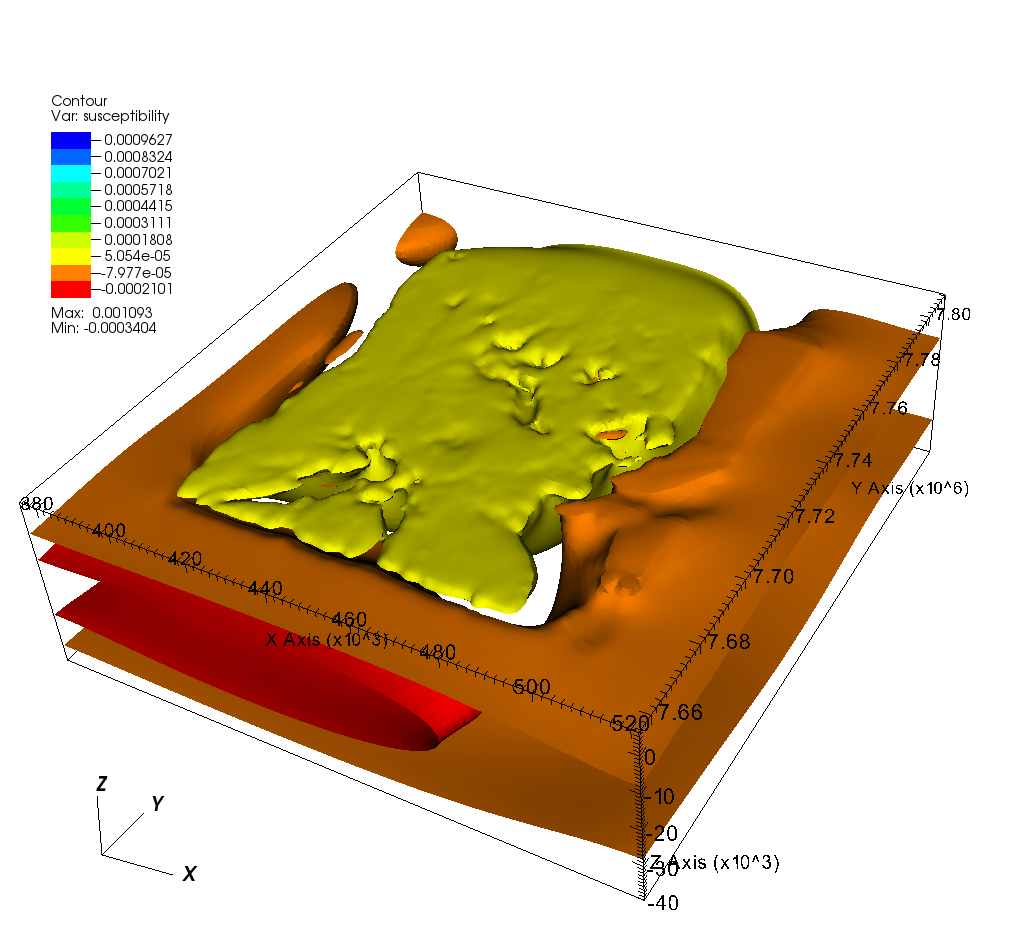
\includegraphics[width=0.45\textwidth]{QLDMagContourMu0001.png}
        }%
        \subfigure[$\mu=0.01$]{%
            \label{FIG:P1:MAG:10 MU001}
            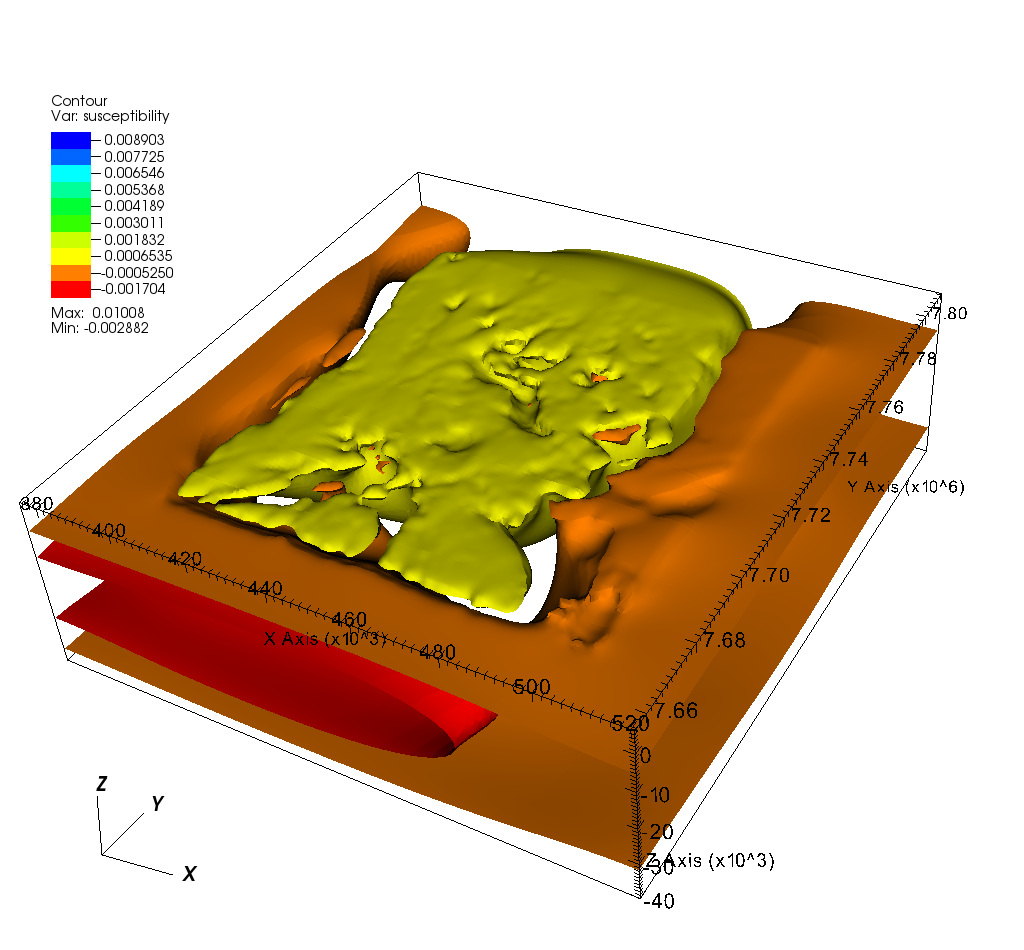
\includegraphics[width=0.45\textwidth]{QLDMagContourMu001.png}
        }\\ %  ------- End of the first row ----------------------%
        \subfigure[$\mu=0.1$]{%
            \label{FIG:P1:MAG:10 MU01}
            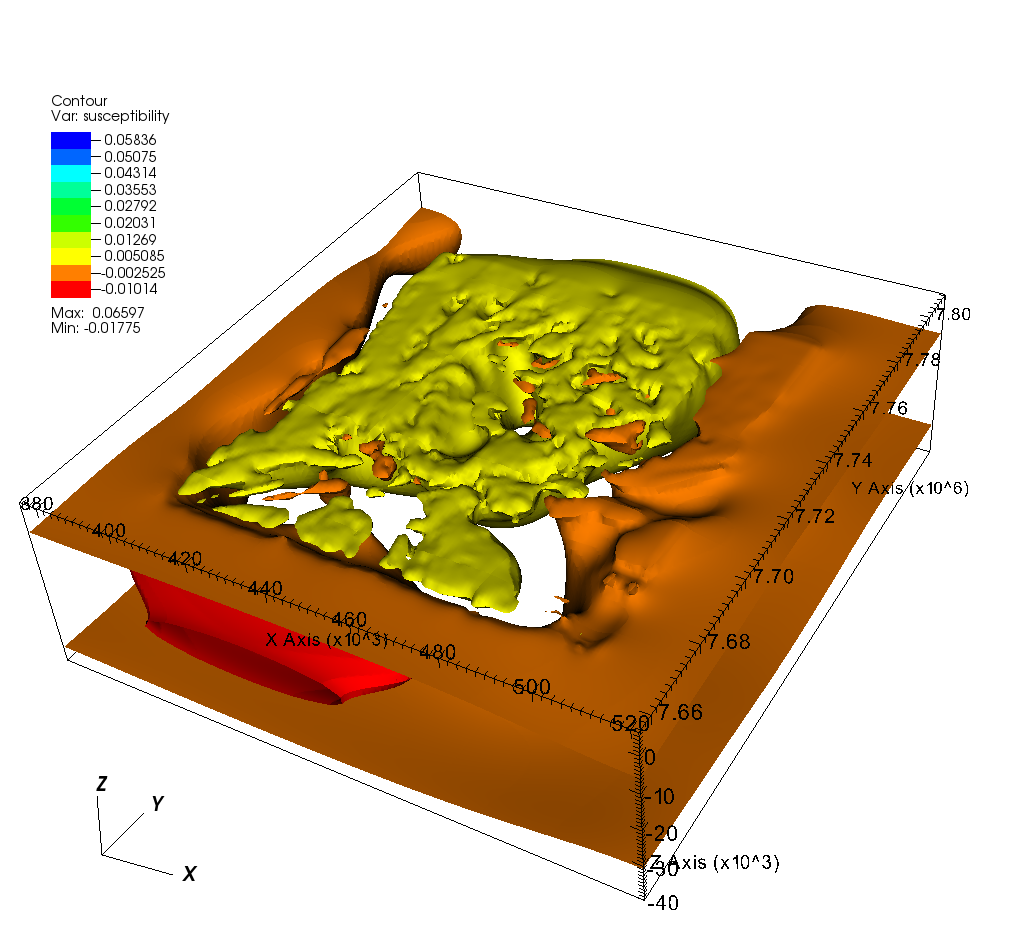
\includegraphics[width=0.45\textwidth]{QLDMagContourMu01.png}
        }%
        \subfigure[$\mu=1.$]{%
            \label{FIG:P1:MAG:10 MU1}
            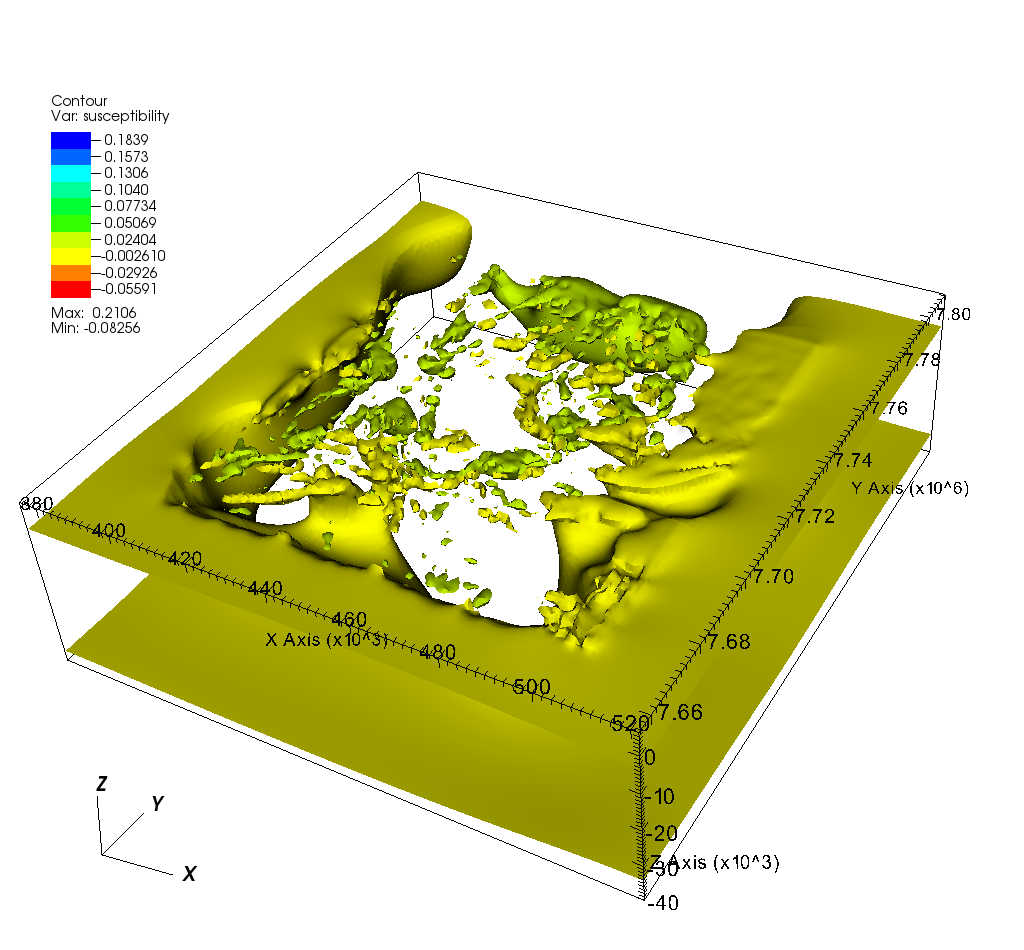
\includegraphics[width=0.45\textwidth]{QLDMagContourMu1.png}
        }\\ %  ------- End of the second row ----------------------%
        \subfigure[$\mu=10.$]{%
            \label{FIG:P1:MAG:10 MU10}
            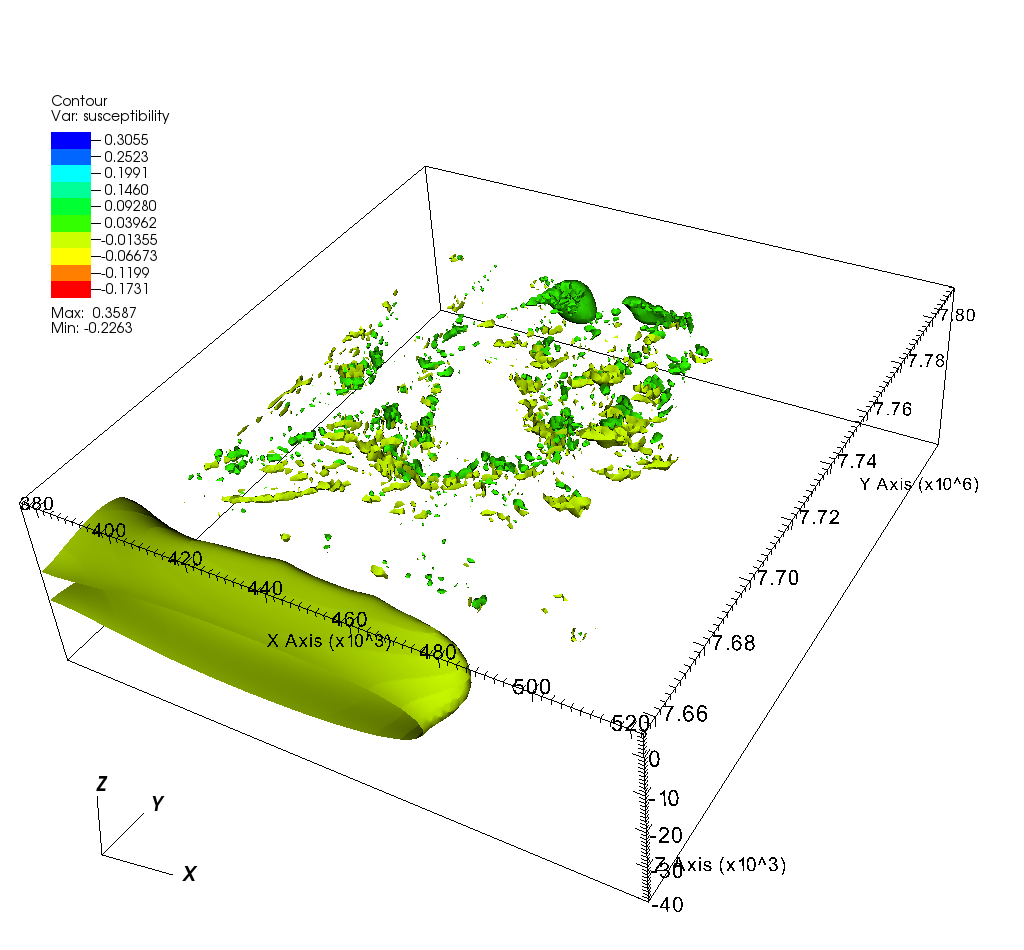
\includegraphics[width=0.45\textwidth]{QLDMagContourMu10.png}
        }%
    \end{center}
    \caption{3-D contour plots of magnetic inversion results with data from
    Figure~\ref{FIG:P1:MAG:0} for various values of the model trade-off
    factor $\mu$. Visualization has been performed in \VisIt.}
    \label{FIG:P1:MAG:10}
\end{figure}

\begin{figure}
    \begin{center}
        \subfigure[$\mu=0.001$]{%
            \label{FIG:P1:MAG:11 MU0001}
            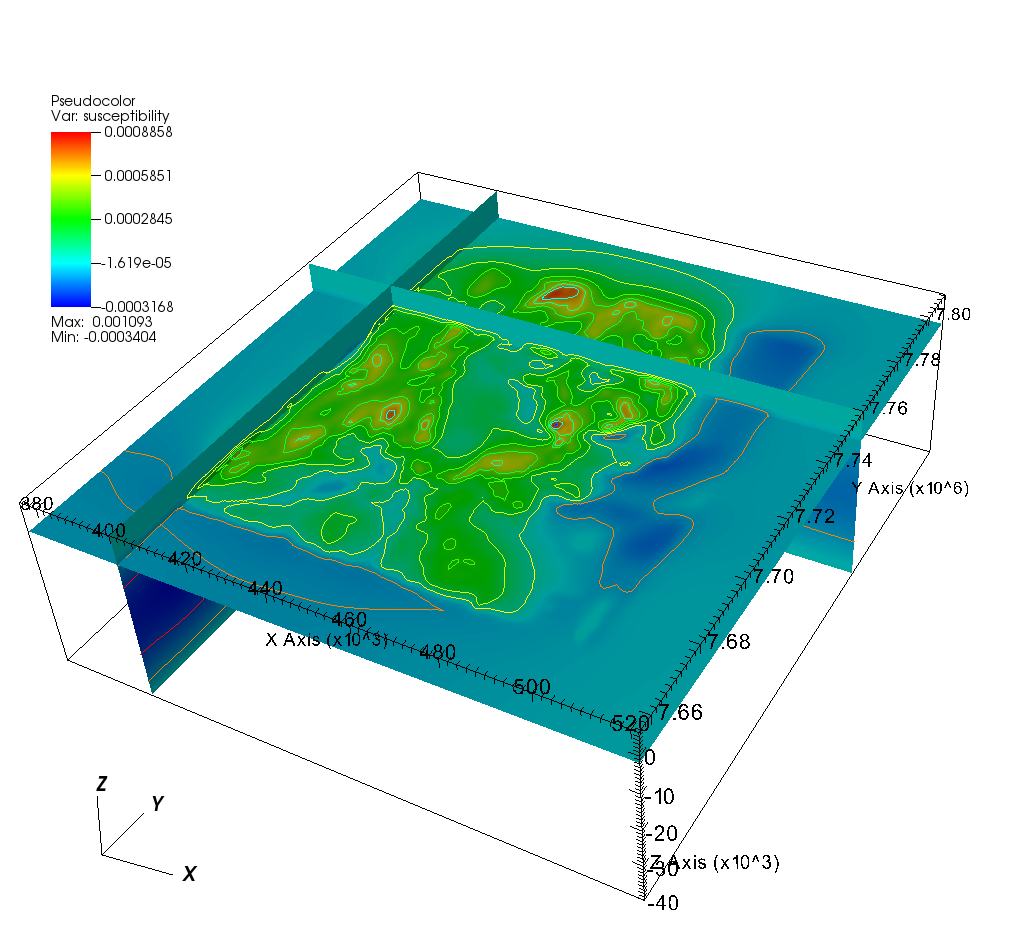
\includegraphics[width=0.45\textwidth]{QLDMagDepthMu0001.png}
        }%
        \subfigure[$\mu=0.01$]{%
            \label{FIG:P1:MAG:11 MU001}
            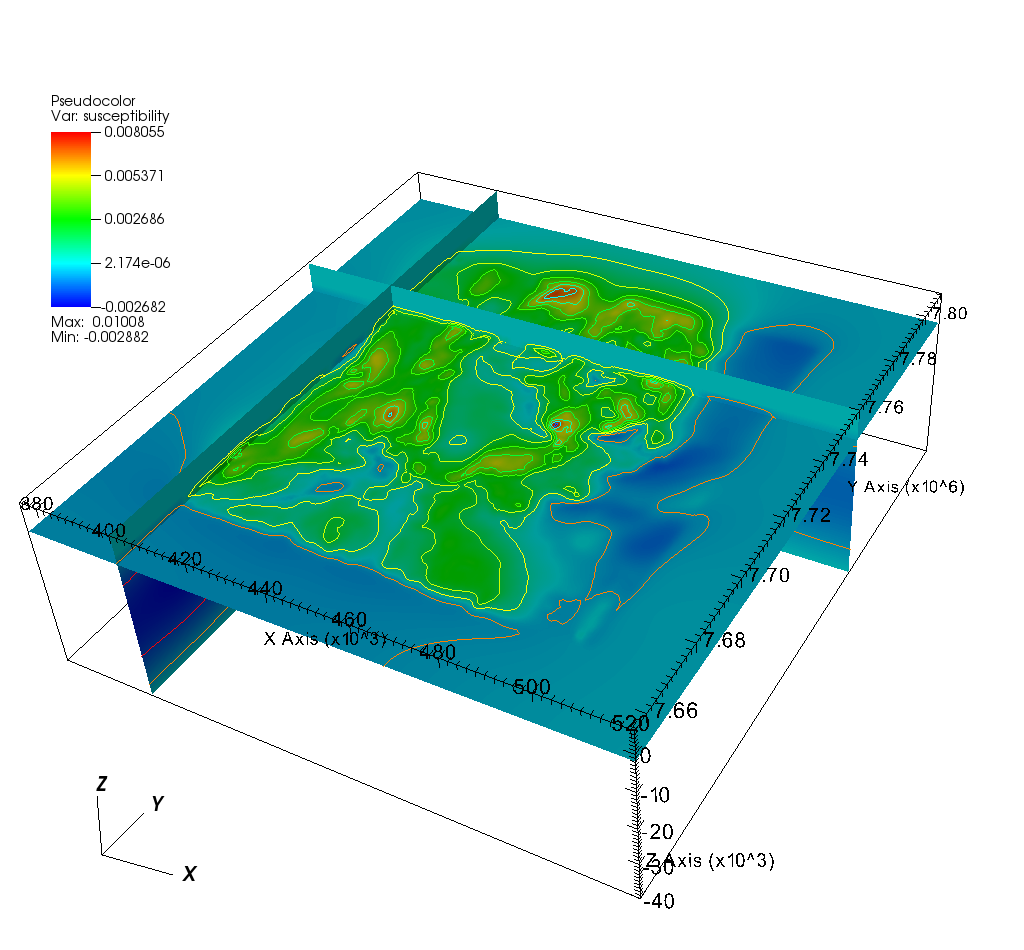
\includegraphics[width=0.45\textwidth]{QLDMagDepthMu001.png}
        }\\ %  ------- End of the first row ----------------------%
        \subfigure[$\mu=0.1$]{%
            \label{FIG:P1:MAG:11 MU01}
            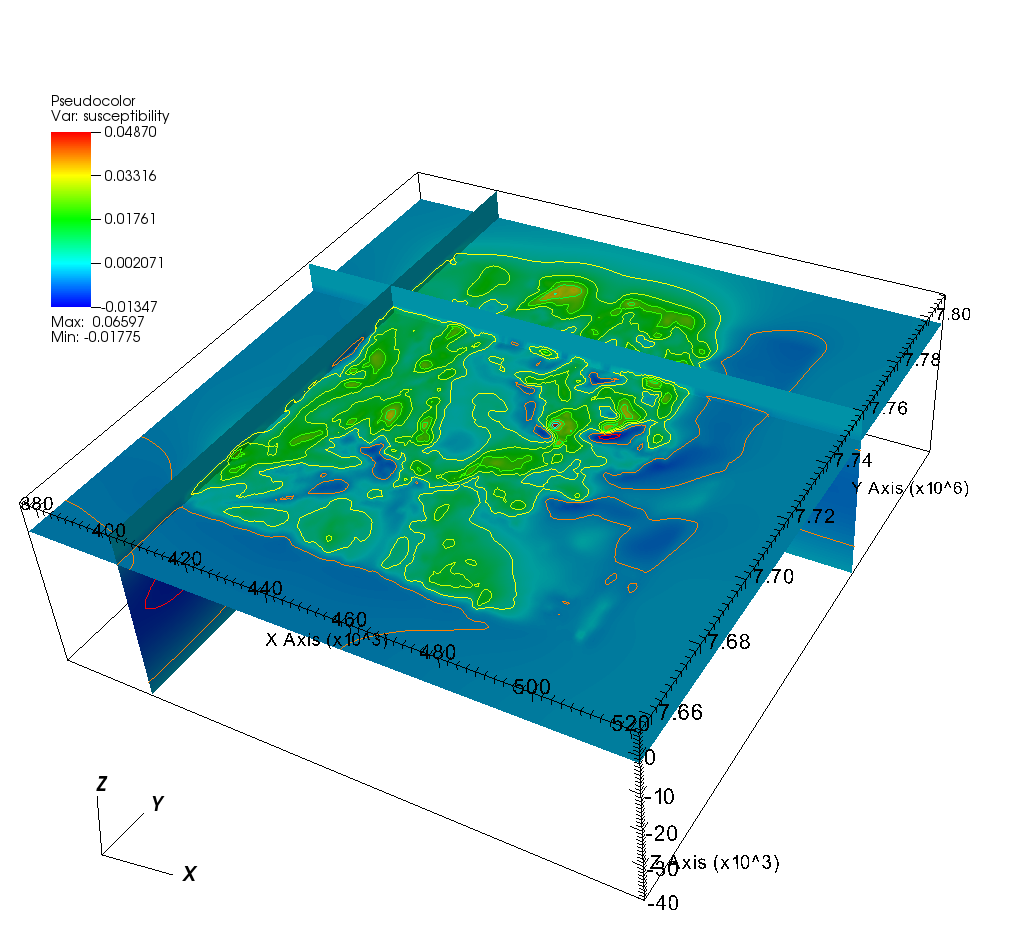
\includegraphics[width=0.45\textwidth]{QLDMagDepthMu01.png}
        }%
        \subfigure[$\mu=1.$]{%
            \label{FIG:P1:MAG:11 MU1}
            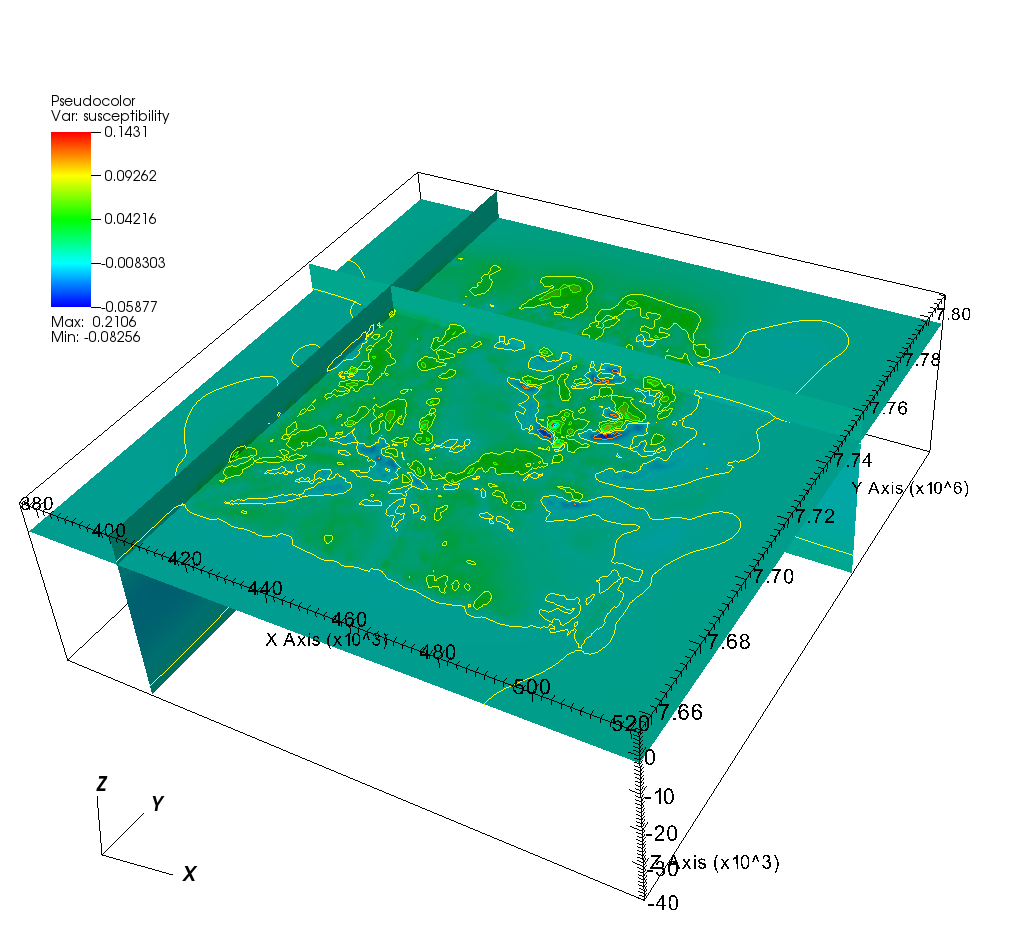
\includegraphics[width=0.45\textwidth]{QLDMagDepthMu1.png}
        }\\ %  ------- End of the second row ----------------------%
        \subfigure[$\mu=10.$]{%
            \label{FIG:P1:MAG:11 MU10}
            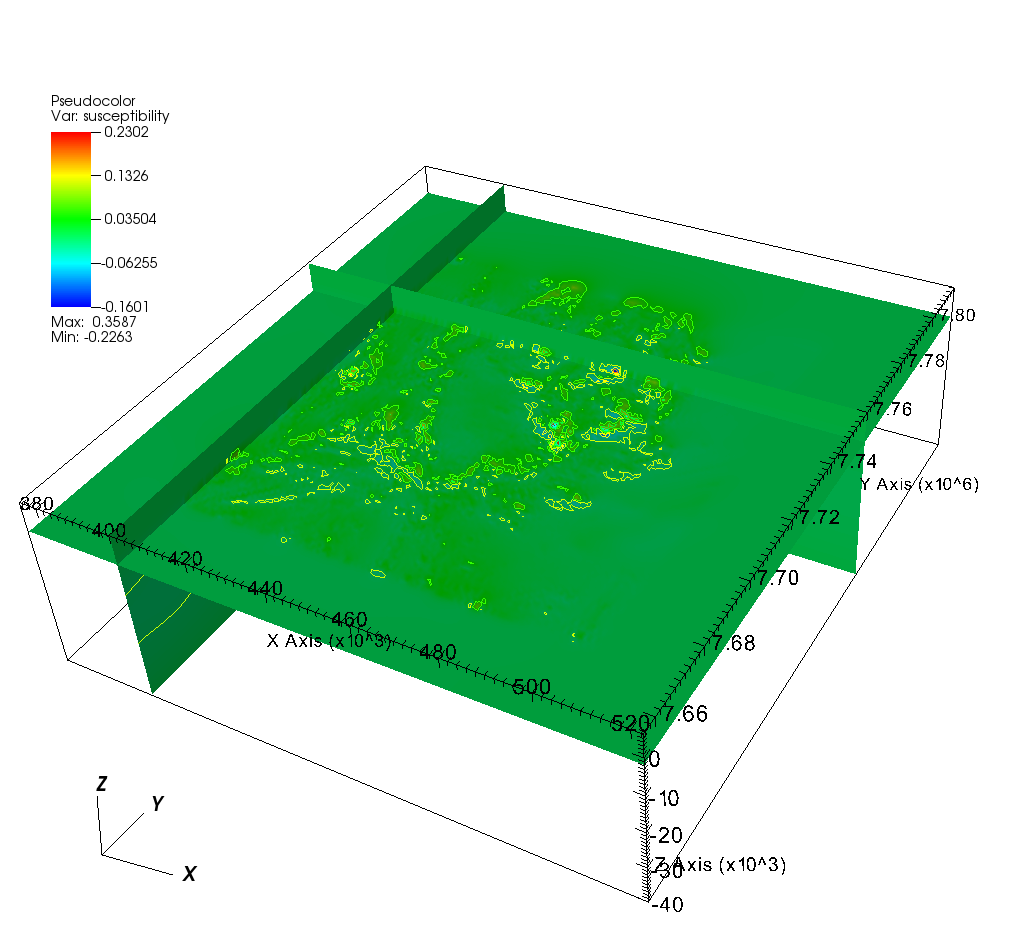
\includegraphics[width=0.45\textwidth]{QLDMagDepthMu10.png}
        }%
    \end{center}
    \caption{3-D slice plots of magnetic inversion results with data from
    Figure~\ref{FIG:P1:MAG:0} for various values of the model trade-off
    factor $\mu$. Visualization has been performed \VisIt.}
    \label{FIG:P1:MAG:11}
\end{figure}

Figures~\ref{FIG:P1:MAG:10} and~\ref{FIG:P1:MAG:11} show results from the
inversion of the magnetic data shown in Figure~\ref{FIG:P1:MAG:0}.
In Figure~\ref{FIG:P1:MAG:10} surface contours are used to represent the
susceptibility while Figure~\ref{FIG:P1:MAG:11} uses contour lines
on a lateral plane intercept and two vertical plane intercepts.
The images show the strong impact of the trade-off factor $\mu$ on the result.
Larger values give more emphasis to the misfit term in the cost function
leading to rougher susceptibility distributions.
The result for $\mu=0.1$ seems to be the most realistic.


\chapter{Joint Inversion}\label{Chp:cook:joint inversion}
This chapter is under development and will become available in the next release.


\part{Reference Guide}\label{part2}
\chapter{Inversion Drivers}\label{chapter:ref:Drivers}

Our task in the inversion\index{inversion} is to find the geological structure within a given three-dimensional region $\Omega$ from given geophysical 
observations\index{observation}. 
The structure is described by a \emph{level set function} $m$\index{level set function}.
This function can be a scalar function or may have several components,
see Chapter~\ref{Chp:ref:regularization} for more details.
Its values are dimensionless and should be between zero and one.
However, the latter condition is not enforced.
Through a mapping (see Chapter~\ref{Chp:ref:mapping}\index{mapping}) the values
of the level set function are mapped onto physical parameter $p^f$\index{physical parameter}.
The physical parameter feeds into one or more forward models\index{forward model}
which return a prediction for the observations, see Chapter~\ref{Chp:ref:forward models}.
An inversion may consider several forward models at once which we call
\emph{joint inversion}\index{joint inversion}.


The level set function describing the actual geological structure is given as
the function which minimizes a particular \emph{cost function}
$J$\index{cost function}.
This cost function is a composition of the difference of the predicted
observations to the actual observations for the relevant forward models, and
the regularization term\index{regularization} which controls the smoothness of
the level set function.
In general the cost function $J$ takes the form
\begin{equation}\label{REF:EQU:INTRO 1}
J(m) = J^{reg}(m) + \sum_{f} \mu^{data}_{f} \cdot J^{f}(p^f)
\end{equation} 
where $J^{f}(p)$ is a measure of the defect of the observations predicted for
the parameter $p^f$ against the observations for forward model $f$, and
$J^{reg}(m)$ is the regularization term.
The weighting factors $\mu^{data}_{f}$ are dimensionless, non-negative
trade-off factors\index{trade-off factor}.
Potentially, values for the trade-off factors are altered during the inversion
process in order to improve the balance between the regularization term and
the data defect terms\footnote{The current version does not support an automated selection 
of trade-off factors}.
The physical parameter $p^f$ depends on the level set function
$m$ in a known form:
\begin{equation}\label{REF:EQU:INTRO 1b}
p^f = M_{f}(m)
\end{equation} 
where $M_f$ is a given mapping. For the case of gravity inversion
the $M_f$ is a simple linear function mapping the level set function $m$ with dimensionless values 
to physical density anomaly values $\rho$.
(see Chapter~\ref{Chp:ref:mapping}\index{mapping}). In its simplest from the mapping is given as 
$\rho = \rho_0 \cdot m$ where $\rho_0$ is a reference density. It is pointed out that 
the inversion techniques applied do not constrain limits to the values of the level set function
although there is the notion that its values are between zero and one. However, 
limits can be enforced to physical parameters using appropriate mappings.

The level set function $m$ and consequently the physical parameters $p^f$ are 
defined over a three dimensional domain $\Omega$ which represented by an \escript 
\class{Domain} object, see \cite{ESCRIPT}. The domain builder methods provide 
functions to build appropriate domains from field data sets, see Section~\ref{Chp:ref:domain builder}.
In general the domain is a rectangular three-dimensional domain where the third dimension $x_2=z$ represents
depth. The $z=0$ surface defines the surface of the earth where $z<0$ is defining the subsurface region and
$z>0$ is defining the region above the surface, see Figure~\ref{fig:cartesianDomain}. In general physical parameters such as
density and susceptibility anomaly are known above the surface, typically assumed to be zero. 
For subregions where a physical parameter is known it is assumed that the corresponding level set function as 
the value zero. If required, non-zero values for the physical parameters can be set using appropriate mapping.      

\begin{figure}[ht]
    \centering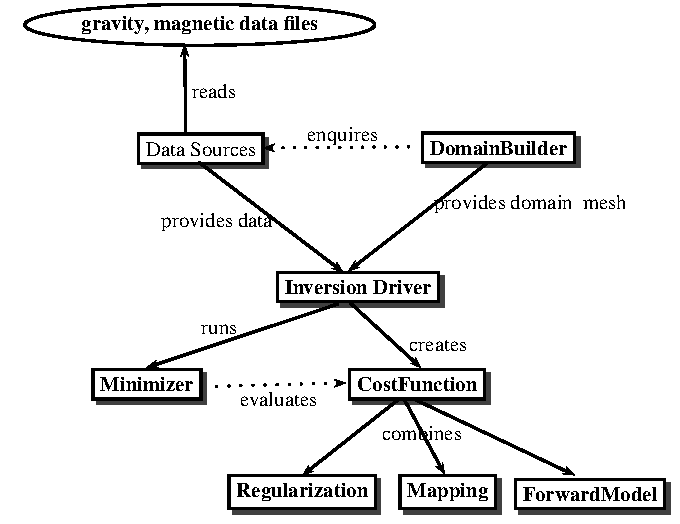
\includegraphics{classdep}
    \caption{Class dependencies}
    \label{fig:classes}
\end{figure} 

\section{Class Dependencies}
For simplification of usage \downunder provides predefined classes that drive inversion for particular 
problems. The usage of this classes is being discussed in Part~\ref{part1}. More details are shown in
Section~\ref{chapter:ref:Drivers:Drivers}. It is the role of the driver class to orchestration an 
inversion. New inversions can easily be implemented by modifying the available drivers.

As illustrated in Figure~\ref{fig:classes} the driver class uses geophysical data as
managed through the \class{DataSource} class (see Chapter~\ref{Chp:ref:data sources}) and 
an \escript domain to define an appropriate
costs function to be minimized. The driver class also run the minimization solver.
The \escript domain~\cite{ESCRIPT} is created using the \class{DomainBuilder}, see Chapter~\ref{Chp:ref:domain builder},
which builds an appropriate domain and mesh based on the geophysical data used in the inversion. 
Based on the inversion to be performed (gravity, magnetic, joint) the 
driver class builds an appropriate cost function $J$ including the regularization term $J^{reg}$, see
\class{Regularization} class in Chapter~\ref{Chp:ref:regularization}, 
the forward models, see Chapter~\ref{Chp:ref:forward models} and
the required mappings, see \class{Mapping} class in Chapter~\ref{Chp:ref:mapping},
to connect the level set function with physical parameters. Finally the driver class calls the
solver to minimize the cost function, see Chapter~\ref{chapter:ref:Minimization}.

The driver classes cover commonly used cases for the convenience of users. In fact, 
more general cases can be implemented in an easy way. Script \examplefile{nodriver.py} is an example 
on how to implement an inversion without using one of the driver classes.   


\section{Domains}


\begin{figure}[ht]
    \centering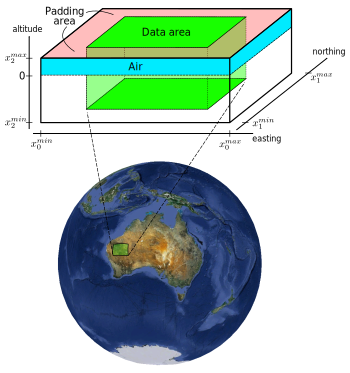
\includegraphics{cartesian}
    \caption{Illustration of domain extents, mapping and padding area}
    \label{fig:cartesianDomain}
\end{figure}

\subsection{Cartesian Domain}
For the Cartesian domain\index{Cartesian Domain} $\Omega$ we assume a flat Earth in the form
\begin{equation} \label{REF:EQU:INTRO 8}
\Omega = [x^{min}_0, x^{max}_0] \times
 [x^{min}_1, x^{max}_1] \times
 [x^{min}_2, x^{max}_2] 
\end{equation} 
and use the Universal Transverse Mercator (UTM) coordinate system\footnote{See
    e.g. \url{http://en.wikipedia.org/wiki/Universal_Transverse_Mercator_coordinate_system}.}
where $x_0$ represents the easting, $x_1$ the northing and $x_2$ the altitude.
In this way, all three coordinates can be given in meters with minimal
distortion when visualizing the domain.
The origin in vertical direction (altitude 0) corresponds to sea level.
A proper inversion set up requires a buffer zone in all dimensions.
Figure~\ref{fig:cartesianDomain} depicts these as areas shaded in red (padding
area) and blue (air buffer).
While the inversion results contain values for the entire domain the buffer zone
should be disregarded when performing any analysis.
In other words, only the region labeled \emph{data area} in
Figure~\ref{fig:cartesianDomain} contains useful information.
Both the thickness of the air layer and the amount of padding in the $x_0$/$x_1$
dimension is configurable when setting up an inversion.





\chapter{Inversion Drivers and Costs Functions}\label{chapter:ref:Drivers}

\begin{classdesc}{SimpleCostFunction}{regularization, mapping, forwardmodel}
    This is a simple cost function with a single continuous (mapped) variable.
    It is the sum of two weighted terms, a single forward model and a single
    regularization term. This cost function is used by the provided gravity
    and magnetic inversion implementations.
\end{classdesc}








 

\chapter{Domains and Coordinate Systems}\label{Chp:ref:coordinates}

If the region of interest is reasonably small a flat Earth can be assumed. In this case
it is sufficient to use a  Cartesian domain\index{Cartesian Domain} $\Omega$ in the form
\begin{equation} \label{REF:EQU:INTRO 8}
\Omega = [x^{min}_0, x^{max}_0] \times
 [x^{min}_1, x^{max}_1] \times
 [x^{min}_2, x^{max}_2] 
\end{equation} 
and use the 
where $x_0$ represents the easting, $x_1$ the northing and $x_2$ the altitude in meters, see Figure~\ref{fig:cartesianDomain}.
It is assumed that data are given is longitude-latitude coordinates which are projected using the   
Universal Transverse Mercator (UTM) coordinate system\footnote{See
    e.g. \url{http://en.wikipedia.org/wiki/Universal_Transverse_Mercator_coordinate_system}.}. 
In this way, all three coordinates can be given in meters with minimal
distortion when visualizing the domain.
The origin in vertical direction (altitude 0) corresponds to sea level.
For some cases, typically if no sufficient data are available, it is appropriate 
to add buffer zones in all dimensions. It can be appropriate to add lateral buffer zones if the 
extend of the area covered by the available data is small. 
Figure~\ref{fig:cartesianDomain} depicts these as areas shaded in red (padding
area) and blue (air buffer).
While the inversion results contain values for the entire domain the buffer zone
should be disregarded when performing any analysis.
In other words, only the region labeled \emph{data area} in
Figure~\ref{fig:cartesianDomain} contains useful information.
Both the thickness of the air layer and the amount of padding in the $x_0$/$x_1$
dimension is configurable when setting up an inversion.

\begin{figure}[ht]
    \centering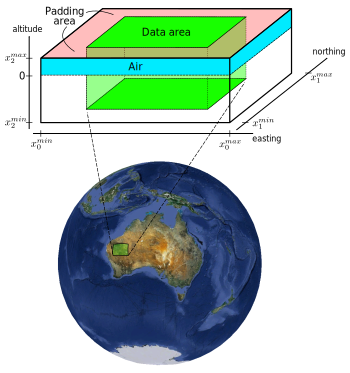
\includegraphics{cartesian}
    \caption{Illustration of domain extents, mapping and padding area}
    \label{fig:cartesianDomain}
\end{figure}

\begin{figure}[t]
    \centering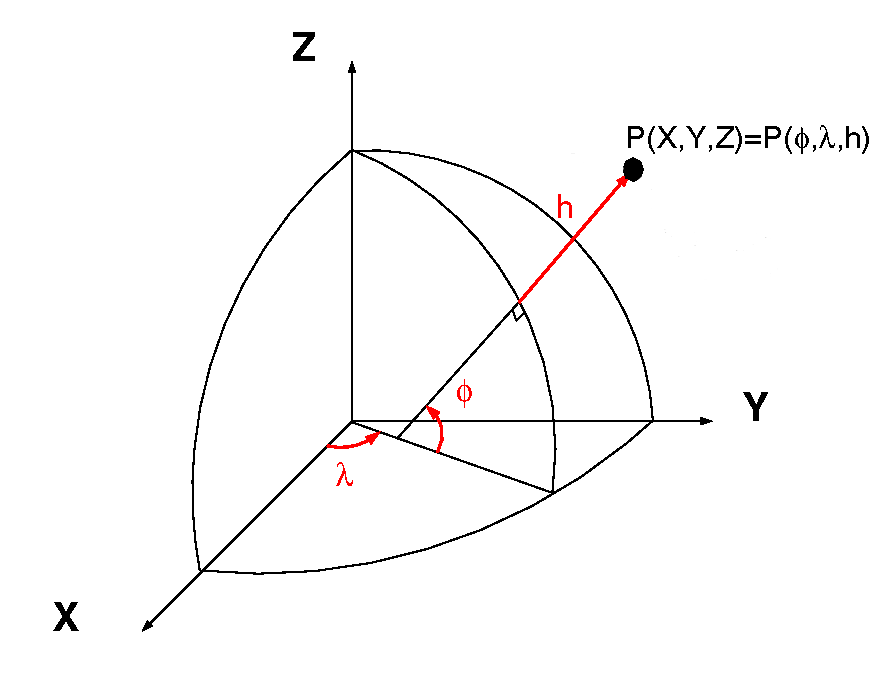
\includegraphics[width=0.7\textwidth]{geosphir}
    \caption{Geodetic coordinates  $( \lambda, \phi,h)$ of a point $P$ with 
cooridnates $(X,Y,Z)=(x_0,x_1,x_2)$ (thanks to the National Geodetic Survey of the National Oceanic and Atmospheric Administration (NOAA), 
see \url{http://www.ngs.noaa.gov/)}.
}
    \label{fig:geodeticDomain}
\end{figure}
For larger areas on the Earth surface it is essential consider the curvature of the region of interest. For this case 
it is appropriate to describe the domain of interest using longitude, latitude and height above Earth surface to describe 
the domain of interest. We use the geodetic coordinates (see Figure~\ref{fig:geodeticDomain}) where the location of a point 
is described by its geodetic latitude $\phi$ (in $deg$), longitude 
$\lambda$ (in $deg$) and geodetic height $h$ (in $km$)~\cite{Featherstone2008a} where we assume
\begin{equation}
  -90^o \le \phi \le 90^o \mbox{ and } -180^o \le \lambda \le -180^o \;.
\end{equation} 
In the following we refer to the $(\phi, \lambda, h)$ as the Geodetic Coordinate system\index{geodetic coordinates}.
In practice we will be interested in a subregion $\Omega$ which is given by the coordinate region   
\begin{equation} \label{REF:EQU:INTRO 8b}
\widehat{\Omega} = 
 [\lambda^{min}, \lambda^{max}] \times [\phi^{min}, \phi^{max}] \times
 [h^{min}, h^{max}] 
\end{equation} 
The Cartesian coordinates $(x_0,x_1,x_2)$ of a point are given as 
\begin{equation}
\begin{array}{rcll}
   x_0 & = &  (N + f_{h}  \cdot  h) & \cdot \cos(f_{a} \cdot  \phi) \cdot  \cos(f_{a} \cdot  \lambda) \\
   x_1 & = &  (N + f_{h}  \cdot  h) & \cdot  \cos(f_{a} \cdot  \phi) \cdot  \sin(f_{a} \cdot  \lambda) \\
   x_2 & = &  (N \cdot (1-e^2) + f_{h}  \cdot  h ) & \cdot  \sin(f_{a} \cdot  \phi)\\
\end{array}
\label{equ:geodetic:1}
\end{equation} 
where $N$ is given as 
\begin{equation}
 N = \frac{a}{\sqrt{1- e^2 \cdot \sin^2(f_{a} \cdot  \phi) }}
\label{equ:geodetic:2}
\end{equation}
with the semi major axis length $a$ and $b$ ($ a \ge b$), and the eccentricity 
\begin{equation} \label{equ:ref:coordinates:100}
e = \sqrt{2f - f^2} \mbox{ with flattening } f = 1-\frac{b}{a} \ge 0
\label{equ:geodetic:3}
\end{equation}
The factors $f_{a}$ and $f_{h}$ consider the change of units from 
$deg$ to $rad$ and $km$ to $m$, respectively.
Notice that the surface of the ellipsoid (Earth) is described by the case $h=0$.  Table~\ref{REF:FIG:REF:10}
shows values for  flattening semi-major axis for the major reference systems of the Earth.

\begin{table}
\begin{center}
\begin{tabular}{c|lll}
Ellipsoid reference & Semi-major axis a & Semi-minor axis b & Inverse flattening (1/f)\\
\hline
GRS 80 & 6 378 137.0 m & 6 356 752.314 140 m & 298.257 222 101\\
WGS 84 & 6 378 137.0 m & 6 356 752.314 245 m & 298.257 223 563
\end{tabular}
\end{center}
\caption{Geodetic Reference Systems of the Earth}\label{REF:FIG:REF:10}
\end{table}

We need to translate any object from the Cartesian coordinates $(x_i)$ in terms of Geodetic Coordinate system
$(\phi, \lambda, h)$. In the following indexes running through $(\phi, \lambda, h)$ are denoted by little Greek letters $\alpha$, 
$\beta$
to separate them from indexes running through the components of the Cartesian coordinates system in little Latin letters.
With this convection the derivative of a function $g$ with respect to the Geodetic coordinates which is given as
\begin{equation}
\begin{array}{rcl}
  g_{,\lambda} & =  & g_{,0} \cdot x_{0,\lambda} + g_{,1} \cdot x_{1,\lambda} + g_{,2} \cdot x_{2,\lambda} \\  
  g_{,\phi} & =  & g_{,0} \cdot x_{0,\phi} + g_{,1} \cdot x_{1,\phi} + g_{,2} \cdot x_{2,\phi} \\
  g_{,h} & =  & g_{,0} \cdot x_{0,h} + g_{,1} \cdot x_{1,h} + g_{,2} \cdot x_{2,h} \\
\end{array}
\end{equation}
via chain rule can be written in the compact form 
\begin{equation}
  g_{,\alpha}   =    g_{,i} \cdot x_{i,\alpha} 
\end{equation}
with
\begin{equation}
 x_{i,\alpha}
= 
\left[
\begin{array}{ccc}
-  R_N \cdot \cos(f_{a} \cdot  \phi) \cdot  \sin(f_{a} \cdot  \lambda) & - R_M \cdot \sin(f_{a} \cdot  \phi) \cdot  \cos(f_{a} \cdot  \lambda) &  f_{h}  \cdot  \cos(f_{a} \cdot  \phi) \cdot  \cos(f_{a} \cdot  \lambda)  \\
 R_N  \cdot  \cos(f_{a} \cdot  \phi) \cdot  \cos(f_{a} \cdot  \lambda) &   -  R_M \cdot  \sin(f_{a} \cdot  \phi) \cdot  \sin(f_{a} \cdot  \lambda) &   f_{h}  \cdot  \cos(f_{a} \cdot  \phi) \cdot  \sin(f_{a} \cdot  \lambda) \\
 0 &  R_M  \cdot  \cos(f_{a} \cdot  \phi) &    f_{h}  \cdot  \sin(f_{a} \cdot  \phi) \\
\end{array}
\right]
\end{equation}
with 
\begin{equation}
R_M = f_{a}  \cdot (M + f_{h}  \cdot h) \mbox{ and }
R_N = f_{a}  \cdot  (N + f_{h}  \cdot h) 
\label{equ:geodetic:5}
\end{equation}
and 
\begin{equation}
 M = \frac{a \cdot  (1-e^2) }{(1- e^2 \cdot \sin^2(f_{a} \cdot  \phi))^{\frac{3}{2}}}
\label{equ:geodetic:5}
\end{equation}
With the coordinate vectors $(u_{\alpha})$ defined as 
\begin{equation}
u_{i \alpha} = d_{\alpha \alpha} x_{i,\alpha}
\end{equation}
and scaling factors 
\begin{equation}
d_{\lambda \lambda} =  \frac{1}{f_{a} \cdot (N + f_{h} \cdot h) \cdot \cos(f_{a} \cdot  \phi)}  \; , 
d_{\phi \phi} = \frac{1}{f_{a} \cdot (M + f_{h} \cdot h)} \mbox{ and }
d_{h h} = \frac{1}{f_{h}}
\end{equation}
we get 
\begin{equation}
g_{,\alpha}   =    g_{,i} u_{i \alpha} \frac{1}{d_{\alpha \alpha}} 
\end{equation}
With the fact that 
\begin{equation}
 u_{i \alpha} u_{j \alpha} = \delta_{ij} \mbox{ and }  u_{i \alpha} u_{i \beta} = \delta_{\alpha \beta}
\end{equation}
\begin{equation}
g_{,i} = d_{\alpha \alpha} g_{,\alpha}  u_{i \alpha} 
\end{equation}
or 
\begin{equation}
g_{,i} = 
\frac{1}{f_{a} \cdot (N + f_{h} \cdot h) \cdot \cos(f_{a} \cdot  \phi) }  g_{,\lambda}  u_{i \lambda} +
\frac{1}{f_{a} \cdot (M + f_{h} \cdot h)}   g_{,\phi}  u_{i \phi} + 
\frac{1}{f_{h}}  u_{i h} 
\end{equation} 
Moreover for integrals we get by substitution rule 
\begin{equation}
dx_0 \; dx_1  \;  dx_2 =\det((x_{i,\alpha}))  \;  d \phi  \;   d\lambda   \;  dh = v \;  d \phi  \;   d\lambda   \;  dh
\end{equation} 
with  $v= \frac{1}{d_{\phi \phi} d_{\lambda \lambda} d_{h h}} =
f_{a}^2 f_{h} (M + f_{h} \cdot h) (N + f_{h} \cdot h) \cdot \cos(f_{a} \cdot  \phi) 
$.
Notice that for a spherical Earth $e=0$ for which $M=N$ is the radius of the Earth and $M+h$ is the distance from
the center \footnote{It is useful to keep in mind that
for the Cartesian cooridnate system $(x_0, x_1, x_2) = (\phi, \lambda, h)$ and $v=1$ and $d_{\alpha \alpha}=1$}. 

\section{Reference Systems}\label{sec:ref:reference systems}
The \class{ReferenceSystem} is an identifier for a coordinate system which is used to define a 
transformation from a rectangular domain $\widehat{\Omega}$ to a subregion at and around the surface of the Earth. 
Although the terminology can be applied to a any orthogonal coordinate system in practice
we have two relevant cases, namely the case the Cartesian coordinate system where no coordinate transformation
is applied ($\widehat{\Omega}= \widehat{\Omega}$) and a Geodetic coordinate system as described above. 
The two class \class{CartesianReferenceSystem} and \class{GeodeticReferenceSystem} as described in the 
next subsection implement a \class{ReferenceSystem}.

\subsection{Cartesian Reference Systems}
\begin{classdesc}{CartesianReferenceSystem}{}
the Cartesian reference coordinate system.
\end{classdesc}

\begin{methoddesc}[GeodeticReferenceSystem]{isCartesian}{}
returns \True 
\end{methoddesc}


\begin{methoddesc}[CartesianReferenceSystem]{isTheSame}{other}
test if \member{other} is also the Cartesian reference coordinate system
\end{methoddesc}


\begin{methoddesc}[CartesianReferenceSystem]{createTransformation}{domain}
creates the appropriate coordinate transformation \class{CartesianCoordinateTransformation} on a given \member{domain}
from the reference coordinate system.
\end{methoddesc}

\subsection{Geodetic Reference Systems}

\begin{classdesc}{GeodeticReferenceSystem}{
  \optional{ a=6378137.0} 
  \optional{, f=1/298.257223563} 
  \optional{, name="WGS84"}
}
initializes a geodetic reference system. 
\member{a} is the length of the semi-major axis in meter.
\member{f} is the flattening, see equation~\ref{equ:ref:coordinates:100}.  
\member{name} sets the name for the reference system 
\end{classdesc}


\begin{methoddesc}[GeodeticReferenceSystem]{isCartesian}{}
returns \False 
\end{methoddesc}


\begin{methoddesc}[GeodeticReferenceSystem]{getSemiMajorAxis}{}
returns the length of semi major axis
\end{methoddesc}

\begin{methoddesc}[GeodeticReferenceSystem]{getSemiMinorAxis}{}
returns the length of semi minor axis
\end{methoddesc}

\begin{methoddesc}[GeodeticReferenceSystem]{getFlattening}{}
returns the flattening
\end{methoddesc}


\begin{methoddesc}[GeodeticReferenceSystem]{isTheSame}{other}
test if \member{other} defines the same reference coordinate system.
\end{methoddesc}

\begin{methoddesc}[GeodeticReferenceSystem]{createTransformation}{domain}
creates the appropriate coordinate transformation \class{GeodeticReferenceSystem}  on a given \member{domain}
from the reference coordinate system.
\end{methoddesc}

\subsection{Short Cuts} 
And some shorts cuts for some standart reference systems:
\begin{funcdesc}{SphericalReferenceSystem}{\optional{R=6378137.0}}
returns the \class{GeodeticReferenceSystem} of a sphere of radius \member{R} in meters.
\end{funcdesc}

\begin{funcdesc}{WGS84ReferenceSystem}{}
returns the \class{GeodeticReferenceSystem} for the WGS84 Ellipsoid, see Table~\ref{REF:FIG:REF:10}.
\end{funcdesc}

\begin{funcdesc}{GRS80ReferenceSystem}{}
returns the \class{GeodeticReferenceSystem} for the GRS80 Ellipsoid, see Table~\ref{REF:FIG:REF:10}.
\end{funcdesc}

\section{Coordinate Transformation}\label{sec:ref:trafo}
A coordinate transformation defines a transformation of a reference domain $\widehat{\Omega}$ using
a coordinate reference system~\footnote{In general any orthogonal coordinate transformation can be supported
by building subclasses of the \class{SpatialCoordinateTransformation}}. The following script shows the usage:
\begin{python}
from escript.ripley import Brick
domain=Brick(10,10, 30, l0=[-35.,-34.], l1=[148.,149], l2=[-40.,40.])
trafo=GeodeticCoordinateTransformation(domain, WGS84ReferenceSystem())
\end{python}
or in a more generic form:
\begin{python}
from escript.ripley import Brick
ref=WGS84ReferenceSystem()
domain=Brick(10,10, 30, l0=[-35.,-34.], l1=[148.,149], l2=[-40.,40])
trafo=ref.createTransformation(domain)
\end{python}
Notice that the coordinate ranges for latitude (\member{l0}) and 
longitude (\member{l1}) are given in degree amd
the range for height $h$ above surface (\member{l2}) in $km$.
The \member{trafo} objects provides now access to the volume factor $v$ and the scaling factors $d_{\alpha, \alpha}$.   
The class \\ \class{GeodeticCoordinateTransformation} has the following interface:
\begin{classdesc}{GeodeticCoordinateTransformation}{domain \optional{, reference=WGS84ReferenceSystem()}}
defines a geodetic coordinate transformation with \member{domain} ($=\widehat{\Omega}$) 
using the reference coordinate system \member{reference}. 
Argument \member{domain} needs to be an \escript \class{Domain} object.
\member{reference}, if present, needs to be a \class{GeodeticReferenceSystem} class object.
\end{classdesc}


\begin{methoddesc}[GeodeticCoordinateTransformation]{isTheSame}{other}
tests of \member{other} defines the same coordinate transformation, i.e. uses the same reference system and the same domain.
\end{methoddesc}


\begin{methoddesc}[GeodeticCoordinateTransformation]{isCartesian}{}
returns \False.
\end{methoddesc}

\begin{methoddesc}[GeodeticCoordinateTransformation]{getDomain}{}
returns the domain of the coordinate transformation.
\end{methoddesc}


\begin{methoddesc}[GeodeticCoordinateTransformation]{getReferenceSystem}{}
returns the reference system used to define the coordinate transformation
\end{methoddesc}


\begin{methoddesc}[GeodeticCoordinateTransformation]{getVolumeFactor}{}
returns the volume factor for the coordinate transformation $v$.
\end{methoddesc}


\begin{methoddesc}[GeodeticCoordinateTransformation]{getScalingFactors}{}
returns the scaling factors $d_{\alpha, \alpha}$.
\end{methoddesc}

\subsection{Cartesian Transformation}
In order to be able to use Cartesian coordinates  within \downunder in the same way like geodetic coordinates 
one can use the class \class{CartesianCoordinateTransformation}.  It defines the same interface 
like the 
\class{GeodeticCoordinateTransformation} class:
\begin{python}
from escript.ripley import Brick
ref=CartesianReferenceSystem()
domain=Brick(10,10, 30, l0=[0.,10000], l1=[0.,10000], l2=[-40000.,40000])
trafo=ref.createTransformation(domain)
\end{python}
Notice that the coordinate ranges for North-South extend (\member{l0}) and 
East_West extend (\member{l1}) and height above ground level (\member{l2})  are given in meters now.

\begin{classdesc}{CartesianCoordinateTransformation}{domain}
defines a Cartesian coordinate transformation with domain \member{domain}. In fact no coordinate transformation is
transformed.  
\end{classdesc}


\begin{methoddesc}[CartesianCoordinateTransformation]{isTheSame}{other}
tests of \member{other} defines the same coordinate transformation, i.e. uses the same reference system and the same domain.
\end{methoddesc}


\begin{methoddesc}[CartesianCoordinateTransformation]{isCartesian}{}
returns \True.
\end{methoddesc}

\begin{methoddesc}[CartesianCoordinateTransformation]{getDomain}{}
returns the domain of the coordinate transformation.
\end{methoddesc}


\begin{methoddesc}[CartesianCoordinateTransformation]{getReferenceSystem}{}
returns the reference system used to define the coordinate transformation (an instance of \class{CartesianReferenceSystem})
\end{methoddesc}


\begin{methoddesc}[CartesianCoordinateTransformation]{getVolumeFactor}{}
returns the volume factor for the coordinate transformation $v$ ($=1$).
\end{methoddesc}


\begin{methoddesc}[CartesianCoordinateTransformation]{getScalingFactors}{}
returns the scaling factors $d_{\alpha \alpha}$ ($=1$).
\end{methoddesc}

%%%%%%%%%%%%%%%%%%%%%%%%%%%%%%%%%%%%%%%%%%%%%%%%%%%%%%%%%%%%%%%%%%%%%%%%%%%%%%
% Copyright (c) 2003-2015 by The University of Queensland
% http://www.uq.edu.au
%
% Primary Business: Queensland, Australia
% Licensed under the Open Software License version 3.0
% http://www.opensource.org/licenses/osl-3.0.php
%
% Development until 2012 by Earth Systems Science Computational Center (ESSCC)
% Development 2012-2013 by School of Earth Sciences
% Development from 2014 by Centre for Geoscience Computing (GeoComp)
%
%%%%%%%%%%%%%%%%%%%%%%%%%%%%%%%%%%%%%%%%%%%%%%%%%%%%%%%%%%%%%%%%%%%%%%%%%%%%%%

\chapter{Minimization Algorithms}\label{chapter:ref:Minimization}
We need to find the level set function $m$ minimizing the cost function $J$ as 
defined in Equation~\ref{REF:EQU:INTRO 1}. The physical parameters $p^f$ and
the data defects are linked through state variables $u^f$ which is given as a
solution of a partial differential equation (PDE) with coefficients depending
on $p_f$. This PDE (or -- in case of several forward models -- this set of PDEs)
defines a constraint in the minimization problem.
In the context of our applications it can be assumed that the PDE is of
'maximum rank', i.e. for a given value of the level set function $m$ there is a
unique value for the state variables $u^f$ as the solution of the forward model.
So from a mathematical point of view the state variable $u^f$ can be eliminated
from the problem and the minimization problem becomes in fact a minimization
problem for the level set function $m$ alone where the physical parameters
which are of most interest in applications can easily be derived from the
solution. However one needs to keep in mind that each evaluation of the cost
function requires the solution of a PDE (an additional PDE solution is required
for the gradient).

In some application cases the optimization problem to be solved defines a
quadratic programming problem which would allow to use a special case of
solvers.
However, for the general scenarios we are interested in here we cannot assume
this simplification and need to be able to solve for a general cost function.
The method used here is the limited-memory Broyden-Fletcher-Goldfarb-Shanno
(\emph{L-BFGS}) method, see~\cite{Nocedal1980}.
This method is a quasi-Newton method.
To implement the method one needs to provide the evaluation of the cost
function $J$ and its gradient $\nabla J$ and dual product $<\cdot,\cdot>$\footnote{A
dual product $<\cdot,\cdot>$ defines a function which assigns a pair $(p,g)$ of a level
set increment $p$ and a gradient $g$ a real number $<p,g>$. It is linear
in the first and linear in the second argument.}
such that for $\alpha \to$ 0 
\begin{equation}\label{EQU:MIN:1}
J(m+\alpha p) = J(m) + \alpha \cdot < p , \nabla J(m)> + o(\alpha)
\end{equation}  
where $p$ is an increment to the level set function\footnote{$o$ denotes the
little o notation see \url{http://en.wikipedia.org/wiki/Big_O_notation}}.
Notice that if $m$ is the unknown solution one has $\nabla J(m)=0$.
Moreover, an approximation of the inverse of the Hessian operator
$\nabla \nabla J(m)$ needs to be provided for a given value of $m$.
In the implementation we don't need to provide the entire operator but for a
given gradient difference $g$ an approximation $h=Hg$ of
$\nabla \nabla J(m))^{-1}g$ needs to be calculated.
This is an approximative solution of the equation $\nabla \nabla J(m)) h=g$
which in variational form is given as 
\begin{equation}\label{EQU:MIN:2}
<p, \nabla \nabla J(m)\; h > = <p, g>
\end{equation}
for all level set increments $p$.
In the cases relevant here, it is a possible approach to make the approximation
$\nabla \nabla J(m) \approx \nabla \nabla J^{reg}(m)$ which can easily be
constructed and the resulting variational Equation~\ref{EQU:MIN:2} can easily
be solved, see Chapter~\ref{Chp:ref:regularization}.

L-BFGS is an iterative method which calculates a sequence of level set
approximations $m_{k}$ which converges towards the unknown level set function
minimizing the cost function.
This iterative process is terminated if certain stopping criteria are fulfilled.
A criterion commonly used is
\begin{equation}\label{EQU:MIN:3a}
\| m_k - m_{k-1} \| \le \|m_k\| \cdot {m\_tol} 
\end{equation}
in order to terminate the iteration after $m_k$ has been calculated.
In this condition $\|.\|$ denotes a norm and $m\_tol$ defines a relative
tolerance. A typical value for $m\_tol$ is $10^{-4}$. Alternatively one can
check for changes in the cost function:
\begin{equation}\label{EQU:MIN:3b}
\mid J(m_k) - J(m_k) \mid \le \mid J(m_k) - J(m_0) \mid \cdot {J\_tol}  
\end{equation}
where ${J\_tol}$ is a given tolerance and $m_0$ is the initial guess of the solution.
As this criterion depends on the initial guess it is not recommended.

\section{Solver Classes}

\begin{classdesc}{MinimizerLBFGS}{%
\optional{J=\None}%
\optional{, m_tol=1e-4}%
\optional{, J_tol=\None}%
\optional{, imax=300}}
constructs an instance of the limited-memory Broyden-Fletcher-Goldfarb-Shanno \emph{L-BFGS} solver.
\member{J} sets the cost function to be minimized, see Section~\ref{chapter:ref:Minimization: costfunction class}.
If not present the cost function needs to be set using the \member{setCostFunction} method.
\member{m_tol} and \member{J_tol} specify the tolerances for the stopping
criteria (see description of \member{setTolerance} below).
\member{imax} sets the maximum number of iteration steps (see
\member{setMaxIterations} below).
\end{classdesc}

\begin{methoddesc}[MinimizerLBFGS]{setTolerance}{\optional{m_tol=1e-4}\optional{, J_tol=\None}}
sets the tolerances for the stopping criteria. 
\member{m_tol} sets the tolerance for the unknown level set Function~\ref{EQU:MIN:3a}.
If \member{m_tol}=\None the tolerance on level set function is not checked.
\member{J_tol} sets the tolerance for the cost function, see Equation~\ref{EQU:MIN:3b}.
If \member{J_tol}=\None tolerance on the cost function is not checked (recommended).
If \member{m_tol} and \member{J_tol} are both set criterion~\ref{EQU:MIN:3a}
and criterion~\ref{EQU:MIN:3b} are both applied to terminate the iteration.
\end{methoddesc}

\begin{methoddesc}[MinimizerLBFGS]{setMaxIterations}{imax}
sets the maximum number of iterations before the minimizer terminates. If 
the maximum number of iteration is reached a \exception{MinimizerMaxIterReached}
exception is thrown.
\end{methoddesc}

\begin{methoddesc}[MinimizerLBFGS]{getResult}{}
returns the solution of the optimization problem.
This method only returns something useful if the optimization process has
completed.
If the iteration failed the last available approximation of the solution is
returned.
\end{methoddesc}

\begin{methoddesc}[MinimizerLBFGS]{getOptions}{}
returns the solver options as a dictionary which contains all available option
names and their current value.
\end{methoddesc}

\begin{methoddesc}[MinimizerLBFGS]{setOptions}{%
\optional{truncation=30}%
\optional{, restart=60}%
\optional{, initialHessian=1}}
sets solver options. \member{truncation} defines number of gradients to keep in memory.
\member{restart} defines the number of iteration steps after which the iteration is restarted.
\member{initialHessian} can be used to provide an estimate for the scale of 
the inverse Hessian. If the cost function provides such an estimate this
option is ignored.
\end{methoddesc}

\begin{methoddesc}[MinimizerLBFGS]{run}{m0}
runs the solution algorithm and returns an approximation of the solution.
\member{m0} is the initial guess to use.
This method may throw an exception if the maximum number of iterations is
reached or a solver breakdown occurs.
\end{methoddesc}

\begin{methoddesc}[MinimizerLBFGS]{logSummary}{}
writes some statistical information to the logger.
\end{methoddesc}

\section{\member{CostFunction} Class Template}\label{chapter:ref:Minimization: costfunction class}

\begin{classdesc}{CostFunction}{}
template of cost function $J$
\end{classdesc}

\begin{methoddesc}[CostFunction]{getDualProduct}{m, g}
returns the dual product $<m,g>$ of \member{m} and \member{g}.
\end{methoddesc}
%
\begin{methoddesc}[CostFunction]{getValue}{m, *args}
returns the value $J(m)$ using pre-calculated values \member{args} for $m$.
\end{methoddesc}
%
\begin{methoddesc}[CostFunction]{getGradient}{m, *args}
returns the gradient $\nabla J$ of $J$ at $m$ using pre-calculated values \member{args} for $m$.
\end{methoddesc}
%
\begin{methoddesc}[CostFunction]{getArguments}{m}
returns pre-calculated values that are shared in the calculation of $J(m)$ and
$\nabla J(m)$.
\end{methoddesc}
%
\begin{methoddesc}[CostFunction]{getNorm}{m}
returns the norm $\|m\|$ of \member{m}.
\end{methoddesc}
%
\begin{methoddesc}[CostFunction]{updateHessian}{}
notifies the class that the Hessian operator needs to be updated in case the
class provides an approximation for the inverse of the Hessian.
\end{methoddesc}
%
\begin{methoddesc}[CostFunction]{getInverseHessianApproximation}{m, g, *args}
returns an approximative evaluation $p$ of the inverse of the Hessian operator
of the cost function for a given gradient $g$ at location $m$.
\end{methoddesc}


% 
%\section{The Nonlinear Conjugate Gradient method}\label{sec:NLCG}
%The steps for NLCG are
%\begin{enumerate}
%    \item Given an initial guess $\mat{x}_0$, compute the steepest descent
%        direction using the gradient: $\mat{p}_0=-\nabla f(\mat{x}_0)$
%    \item Perform an inexact \emph{line search} (see Section~\ref{sec:LineSearch}) to obtain the step
%        length $\alpha_i$ which loosely minimizes $f(\mat{x}_i+\alpha_i \mat{d}_i)$
%    \item Update the position: $\mat{x}_{i+1}=\mat{x}_i+\alpha_i \mat{d}_i$
%    \item Update the conjugate direction: $\mat{d}_{i+1}=-\nabla f(\mat{x}_{i+1})+\beta_{i+1} \mat{d}_i$\label{CGupdate}
%\end{enumerate}

%\flushleft There are many choices for the CG update parameter $\beta_{i+1}$ in step
%\ref{CGupdate} above, see \cite{Hager2006} for a discussion. An efficient
%choice, proposed by Polak and Ribi\`{e}re, is:
%\begin{equation*}
%    \beta_{i+1}=\text{max}\left\{\frac{\nabla f^T(\mat{x}_{i+1})(\nabla f(\mat{x}_{i+1})-\nabla f(\mat{x}_i))}{\| \nabla f(\mat{x}_i)\|}, 0\right\}
%\end{equation*}

\section{The L-BFGS Algorithm}

%\section{Limited-Memory BFGS Method}\label{sec:LBFGS}
The L-BFGS algorithm looks as follows (see also~\cite{Nocedal1980})\index{L-BFGS}:
\begin{algorithm}
    \mbox{L-BFGS}
    \begin{program}
        \BEGIN
        \text{Input: initial guess $x_0$ and integer $m$};
        \text{Allocate $m$ vector pairs \{$s_i$, $g_i$\}};
        k \leftarrow 0;
        H_0 \leftarrow I;
        \WHILE \NOT\text{converged} \DO
        p_k \leftarrow |twoLoop|(\{s, g\});
        \alpha_k \leftarrow |lineSearch|(m_k, p_k); \rcomment{See Section~\ref{sec:LineSearch}}
        m_{k+1} \leftarrow m_k+\alpha_k p_k;
        \IF k> truncation
        \THEN
            |Discard the vector pair | \{s_{k-truncation}, g_{k-truncation}\} | from storage|;
        \FI
        s_k \leftarrow m_{k+1}-m_k;
        g_k \leftarrow \nabla J_{k+1}-\nabla J_k;
        k \leftarrow k+1;
        \OD
        \WHERE
        \FUNCT |twoLoop|(\{s, g\}) \BODY
            \EXP q \leftarrow \nabla J_k;
            \FOR i=k-1, k-2, \ldots, k-truncation \DO
            \rho_i \leftarrow \frac{1}{<s_i, g_i>};
            \alpha_i \leftarrow \rho_i <s_i, q>;
            q \leftarrow q-\alpha_i\cdot  g_i;
            \OD
            r \leftarrow H q;
            \FOR i = k-truncation, k-truncation+1, \ldots, k-1 \DO
            \beta \leftarrow \rho_i \cdot <r,g_i>;
            r \leftarrow r + s_i \cdot (\alpha_i - \beta)
            \OD
            r \ENDEXP \ENDFUNCT
        \END
    \end{program}
\end{algorithm}

\subsection{Line Search}\label{sec:LineSearch}
The line search procedure minimizes the function $\phi(\alpha)$ for a given
level set function $m$ and search direction $p$, see \cite{Nocedal2006},
\cite{MoreThuente1992} with
\begin{equation}\label{EQU:MIN:22}
\phi(\alpha) = J(m+ \alpha \cdot  p)
\end{equation}
Notice that 
\begin{equation}\label{EQU:MIN:23}
\phi'(\alpha) = < p , \nabla J(m+\alpha \cdot p)> \; .
\end{equation}

\begin{algorithm}
    \mbox{Line Search that satisfies strong Wolfe conditions}
    \begin{program}
        \BEGIN
        \text{Input: $\alpha_{max}>0, 0<c_1<c_2<1$};
        i \leftarrow 1;
        \WHILE 1 \DO
        \IF \phi(\alpha_i) > \phi(0)+c_1 \alpha_i \phi'(0) \OR
            (\phi(\alpha_i) \ge \phi(\alpha_{i-1}) \AND i>1)
        \THEN
            \alpha_* \leftarrow |zoom|(\alpha_{i-1}, \alpha_i);
            |break|;
        \FI
        \IF \|\phi'(\alpha_i)\| \le -c_2\phi'(0)
        \THEN
            \alpha_* \leftarrow \alpha_i;
            |break|;
        \FI
        \IF \phi'(\alpha_i) \ge 0
        \THEN
            \alpha_* \leftarrow |zoom|(\alpha_i, \alpha_{i-1});
            |break|;
        \FI
        \alpha_{i+1} = 2\alpha_i;
        i \leftarrow i+1;
        \OD
        \WHERE
        \FUNCT |zoom|(\alpha_{lo}, \alpha_{hi}) \BODY
            \WHILE 1 \DO
                \EXP \alpha_j \leftarrow \alpha_{lo}+\frac{\alpha_{hi}-\alpha_{lo}}{2};
                \IF \phi(\alpha_j) > \phi(0)+c_1 \alpha_j\phi'(0) \OR %
                    \phi(\alpha_j) \ge \phi(\alpha_{lo})
                \THEN
                    \alpha_{hi} \leftarrow \alpha_j;
                \ELSE
                    \IF \|\phi'(\alpha_j)\| \le -c_2\phi'(0)
                    \THEN
                        \alpha_* \leftarrow \alpha_j;
                        |break|;
                    \FI
                    \IF \phi'(\alpha_j)(\alpha_{hi}-\alpha_{lo}) \ge 0
                    \THEN
                        \alpha_{hi} \leftarrow \alpha_{lo};
                    \FI
                    \alpha_{lo}=\alpha_j;
                \FI
            \OD
            \ENDEXP \ENDFUNCT
        \END
    \end{program}
\end{algorithm}


\chapter{Cost Function}\label{chapter:ref:inversion cost function}
The general form of the cost function minimized in the inversion is given in the form (see also Chapter~\ref{Chp:ref:introduction})
\begin{equation}\label{REF:EQU:DRIVE:10}
J(m) = J^{reg}(m) + \sum_{f} \mu^{data}_{f} \cdot J^{f}(p^f)
\end{equation} 
where $m$ represents the level set function, $J^{reg}$ is the regularization term, see Chapter~\ref{Chp:ref:regularization},
and $J^{f}$ are a set of forward problems, see Chapter~\ref{Chp:ref:forward models} depending of 
physical parameters $p^f$.  The physical parameters $p^f$ are known functions 
of the  level set function $m$ which is the unknown to be calculated by the optimization process. 
$\mu^{data}_{f}$ are trade-off factors. It is pointed out that the regularization term includes additional trade-off factors 
The \class{InversionCostFunction} is class to define cost functions of an inversion. It is pointed out that
the \class{InversionCostFunction} class implements the \class{CostFunction} template class, see Chapter~\ref{chapter:ref:Minimization}.

In the simplest case there is a single forward model using a single physical parameter which is 
derived form single-values level set function. The following script snippet shows the creation of the
\class{InversionCostFunction} for the case of a gravity inversion:
\begin{verbatim}
p=DensityMapping(...)
f=GravityModel(...)
J=InversionCostFunction(Regularization(...), \
                        mappings=p, \
                        forward_models=f)
\end{verbatim}
The argument \verb|...| refers to an appropriate argument list.

If two forward models are coming into play using two different physical parameters 
the \member{mappings} and \member{forward_models} are defined as lists in the following form:
\begin{verbatim}
p_rho=DensityMapping(...)
p_k=SusceptibilityMapping(...)
f_mag=MagneticModel(...)
f_grav=GravityModel(...)

J=InversionCostFunction(Regularization(...), \
                        mappings=[p_rho, p_k], \
                        forward_models=[(f_mag, 1), (f_grav,0)])
\end{verbatim}
Here we define a joint inversion of gravity and magnetic data. \member{forward_models} is given as a list of
a tuple of a forward model and an index which referring to parameter in the \member{mappings} list to be used as an input.
The magnetic forward model \member{f_mag} is using the the second parameter (=\member{p_k}) in \member{mappings} list.
In this case the physical parameters are defined by a single-valued level set function. It is also possible
to link physical parameters to components of a level set function:
\begin{verbatim}
p_rho=DensityMapping(...)
p_k=SusceptibilityMapping(...)
f_mag=MagneticModel(...)
f_grav=GravityModel(...)

J=InversionCostFunction(Regularization(numLevelSets=2,...), \
                        mappings=[(p_rho,0), (p_k,1)], \
                        forward_models=[[(f_mag, 1), (f_grav,0)])   
\end{verbatim}
The \member{mappings} argument is now a list of pairs where the first pair entry specifies the parameter mapping and
the second pair entry specifies the index of the component of the level set function to be used to evaluate the parameter.
In this case the level set function has two components, where the density mapping uses the first component of the level set function 
while the susceptibility mapping uses the second component.

The \class{InversionCostFunction} API is defined as follows:

\begin{classdesc}{InversionCostFunction}{regularization, mappings, forward_models}
Constructor for the inversion cost function. \member{regularization} sets the regularization to be used, see Chapter~\ref{Chp:ref:regularization}.
\member{mappings} is a list of pairs where each pair comprises of a 
physical parameter mapping (see Chapter~\ref{Chp:ref:mapping}) and an index which refers to the component of level set function
defined by the \member{regularization} to be used to calculate the corresponding physical parameter. If 
the level set function has a single component the index can be omitted. If in addition there is a single physical parameter
the mapping can be given instead of a list. \member{forward_models} is a list of pairs where the 
first pair component is a forward model ( see Chapter~\ref{Chp:ref:forward models}) and the second 
pair component referring to the physical parameter in the \member{mappings} list providing the  physical parameter for the model.
If a single physical parameter is present the index can be omitted. If in addition a single  forward model is used this
forward model can be assigned to \member{forward_models} in replacement of a list.
\end{classdesc}


\begin{methoddesc}[InversionCostFunction]{getDomain}{}
        """
        returns the domain of the cost function
        :rtype: 'Domain`
        """
        self.regularization.getDomain()
\end{methoddesc}
        
\begin{methoddesc}[InversionCostFunction]{getNumTradeOffFactors}{}
        """
        returns the number of trade-off factors being used including the
        trade-off factors used in the regularization component.

        :rtype: ``int``
        """
        return self.__num_tradeoff_factors
\end{methoddesc}

 \begin{methoddesc}[InversionCostFunction]{getForwardModel}{idx=None}
        """
        returns the *idx*-th forward model.

        :param idx: model index. If cost function contains one model only `idx`
                    can be omitted.
        :type idx: ``int``
        """
        if idx==None: idx=0
        f=self.forward_models[idx]
        if isinstance(f, ForwardModel): 
              F=f
        else:
              F=f[0]
        return F
\end{methoddesc}
        
\begin{methoddesc}[InversionCostFunction]{getRegularization}{}
        """
        returns the regularization
        """
        return self.regularization
\end{methoddesc}

        
\begin{methoddesc}[InversionCostFunction]{setTradeOffFactorsModels}{mu=None}
        """
        sets the trade-off factors for the forward model components.
        
        :param mu: list of the trade-off factors. If not present ones are used.
        :type mu: ``float`` in case of a single model or a ``list`` of ``float``
                  with the length of the number of models.
        """
        if mu==None:
            self.mu_model=np.ones((self.numModels, )) 
        else:
            if self.numModels > 1:
               mu=np.asarray(mu)
               if min(mu) > 0:
                  self.mu_model= mu
               else:
                  raise ValueError("All value for trade-off factor mu must be positive.")
            else:
              mu=float(mu)
              if mu > 0:
                  self.mu_model= [mu, ]
              else:
                  raise ValueError("Trade-off factor must be positive.") 
\end{methoddesc}
           
\begin{methoddesc}[InversionCostFunction]{setTradeOffFactorsRegularization}{mu=None, mu_c=None}
        """
        sets the trade of factors for the regularization component of the cost
        function, see `Regularization` for details.
        
        :param mu: trade-off factors for the level-set variation part 
        :param mu_c: trade-off factors for the cross gradient variation part 
        """
        self.regularization.setTradeOffFactorsForVariation(mu)
        self.regularization.setTradeOffFactorsForCrossGradient(mu_c)
\end{methoddesc}
        
\begin{methoddesc}[InversionCostFunction]{setTradeOffFactors}{mu=None}
        """
        sets the trade-off factors for the forward model and regularization
        terms. 

        :param mu: list of trade-off factors. 
        :type mu: ``list`` of ``float``
        """
        if mu is None:
            mu=np.ones((self.__num_tradeoff_factors,))
        self.setTradeOffFactorsModels(mu[:self.numModels])
        self.regularization.setTradeOffFactors(mu[self.numModels:])
\end{methoddesc}

\begin{methoddesc}[InversionCostFunction]{createLevelSetFunction}{*props}
        """
        returns an instance of an object used to represent a level set function
        initialized with zeros. Components can be overwritten by physical
        properties 'props'. If present entries must correspond to the
        `mappings` arguments in the constructor. Use `None` for properties for
        which no value is given.
        """
        m=self.regularization.getPDE().createSolution()
        if len(props) > 0:
           for i in xrange(self.numMappings): 
              if props[i]: 
                  mm=self.mappings[i]
                  if isinstance(mm, Mapping):
                      m=mm.getInverse(props[i])
                  elif len(mm) == 1:
                      m=mm[0].getInverse(props[i])
                  else:
                      m[mm[1]]=mm[0].getInverse(props[i])
        return m
\end{methoddesc}
    
\begin{methoddesc}[InversionCostFunction]{getProperties}{m, return_list=False}
        """
        returns a list of the physical properties from a given level set
        function *m* using the mappings of the cost function.
        
        :param m: level set function
        :type m: `Data`
        :param return_list: if True a list is returned. 
            def _:type return_list: `bool`
        :rtype: `list` of `Data`
        """
        props=[]
        for i in xrange(self.numMappings): 
           mm=self.mappings[i]
           if isinstance(mm, Mapping):
               p=mm.getValue(m)
           elif len(mm) == 1:
               p=mm[0].getValue(m)
           else:
               p=mm[0].getValue(m[mm[1]])
           props.append(p)
        if self.numMappings > 1 or return_list:
           return props
        else:
           return props[0]
\end{methoddesc}
           
\begin{methoddesc}[InversionCostFunction]{getDualProduct}{x, r}
        """
        Returns the dual product, see `Regularization.getDualProduct`

        :type x: `Data`
        :type r: `ArithmeticTuple`             
        :rtype: `float`
        """
        return self.regularization.getDualProduct(x, r)
\end{methoddesc}

\begin{methoddesc}[InversionCostFunction]{getArguments}{m}
        """
        returns pre-computed values that are shared in the calculation of
        *J(m)* and *grad J(m)*. In this implementation returns a tuple with the
        mapped value of ``m``, the arguments from the forward model and the
        arguments from the regularization.
        
        :param m: current approximation of the level set function
        :type m: `Data`
        :return: tuple of of values of the parameters, pre-computed values for the forward model and
                 pre-computed values for the regularization
        :rtype: `tuple`
        """
        args_reg=self.regularization.getArguments(m)

        props=self.getProperties(m, return_list=True)
        args_f=[]
        for i in xrange(self.numModels):
           f=self.forward_models[i]
           if isinstance(f, ForwardModel): 
              aa=f.getArguments(props[0])
           elif len(f) == 1:
              aa=f[0].getArguments(props[0])
           else:
              idx = f[1]
              f=f[0]
              if isinstance(idx, int):
                 aa=f.getArguments(props[idx])
              else:
                 pp=tuple( [ props[i] for i in idx] )
                 aa=f.getArguments(*pp)
           args_f.append(aa)
           
        return props, args_f, args_reg
\end{methoddesc}

\begin{methoddesc}[InversionCostFunction]{getValue}{m, *args}
        """
        Returns the value *J(m)* of the cost function at *m*.
        If the pre-computed values are not supplied `getArguments()` is called.

        :param m: current approximation of the level set function
        :type m: `Data`
        :param args: tuple of of values of the parameters, pre-computed values for the forward model and
                 pre-computed values for the regularization
        :rtype: `float`
        """

        if len(args)==0:
            args=self.getArguments(m)
        
        props=args[0]
        args_f=args[1]
        args_reg=args[2]
        
        J = self.regularization.getValue(m, *args_reg)
        print "J_reg = %e"%J
                
        for i in xrange(self.numModels):
                 
           f=self.forward_models[i]
           if isinstance(f, ForwardModel): 
              J_f = f.getValue(props[0],*args_f[i])
           elif len(f) == 1:
              J_f=f[0].getValue(props[0],*args_f[i])
           else:
              idx = f[1]
              f=f[0]
              if isinstance(idx, int):
                 J_f = f.getValue(props[idx],*args_f[i])
              else:
                 args=tuple( [ props[j] for j in idx] + args_f[i])
                 J_f = f.getValue(*args)
           print "J_f[%d] = %e"%(i, J_f)
           print "mu_model[%d] = %e"%(i, self.mu_model[i])
           J += self.mu_model[i] * J_f
           
        return   J
\end{methoddesc}

\begin{methoddesc}[InversionCostFunction]{getGradient}{m, *args}
        """
        returns the gradient of the cost function  at *m*.
        If the pre-computed values are not supplied `getArguments()` is called.

        :param m: current approximation of the level set function
        :type m: `Data`
        :param args: tuple of of values of the parameters, pre-computed values for the forward model and
                 pre-computed values for the regularization
                 
        :rtype: `ArithmeticTuple`
        """
        if len(args)==0:
            args = self.getArguments(m)
         
        props=args[0]
        args_f=args[1]
        args_reg=args[2]
        
        g_J = self.regularization.getGradient(m, *args_reg) 
        p_diffs=[]
        for i in xrange(self.numMappings): 
           mm=self.mappings[i]
           if isinstance(mm, Mapping):
               dpdm = mm.getDerivative(m)
           elif len(mm) == 1:
               dpdm = mm[0].getDerivative(m)
           else:
               dpdm = mm[0].getDerivative(m[mm[1]])
           p_diffs.append(dpdm)
           
        Y=g_J[0]   
        for i in xrange(self.numModels):
           mu=self.mu_model[i] 
           f=self.forward_models[i]
           if isinstance(f, ForwardModel): 
              Ys= f.getGradient(props[0],*args_f[i]) * p_diffs[0] * mu
              if self.numLevelSets == 1 :
                 Y +=Ys
              else:
                  Y[0] +=Ys
           elif len(f) == 1:
              Ys=f[0].getGradient(props[0],*args_f[i]) * p_diffs[0]  * mu
              if self.numLevelSets == 1 :
                 Y +=Ys
              else:
                  Y[0] +=Ys
           else:
              idx = f[1]
              f=f[0]
              if isinstance(idx, int):
                 Ys = f.getGradient(props[idx],*args_f[i]) * p_diffs[idx] * mu 
                 if self.numLevelSets == 1 :
                     if idx == 0:
                         Y+=Ys
                     else:
                         raise IndexError("Illegal mapping index.")
                 else:
                     Y[idx] += Ys 
              else:
                 args=tuple( [ props[j] for j in idx] + args_f[i])
                 Ys = f.getGradient(*args)
                 for ii in xrange(len(idx)):
                     Y[idx[ii]]+=Ys[ii]* p_diffs[idx[ii]]  * mu

        return g_J
\end{methoddesc}


\begin{methoddesc}[InversionCostFunction]{getInverseHessianApproximation}{m, r, *args}
        """
        returns an approximative evaluation *p* of the inverse of the Hessian operator of the cost function
        for a given gradient type *r* at a given location *m*: *H(m) p = r*

        :param m: level set approximation where to calculate Hessian inverse
        :type m: `Data`
        :param r: a given gradient
        :type r: `ArithmeticTuple`
        :param args: tuple of of values of the parameters, pre-computed values for the forward model and
                 pre-computed values for the regularization
        :rtype: `Data`
        :note: in the current implementation only the regularization term is
               considered in the inverse Hessian approximation.

        """
        m=self.regularization.getInverseHessianApproximation(m, r, *args[2])
        return m

\end{methoddesc}
        
\begin{methoddesc}[InversionCostFunction]{getNorm}{m}
        """
        returns the norm of ``m``

        :param m: level set function
        :type m: `Data`
        :rtype: ``float``
        """

\end{methoddesc}

\chapter{Data Sources}\label{Chp:ref:data sources}

At the source of every inversion is data in the form of gravity anomaly or
magnetic flux density values for at least a part of the region of interest.
These usually come from surveys and are preprocessed to correct for various
factors and distortions.
This chapter provides an overview of the classes related to data input for
inversions.

\section{Overview}
The inversion module comes with a number of classes that can read gridded
(raster) data on a 2-dimensional plane from file or provide artificial values
for testing purposes. These classes all derive from the abstract
\class{DataSource} class and override methods that return information about
the data and the values themselves.
The \class{DomainBuilder} class is responsible for creating an \escript domain
with a suitable grid spacing and spatial extents that include all data sources
attached to it (see Figure~\ref{fig:domainBuilder}).
%
\begin{figure}[ht]
    \centering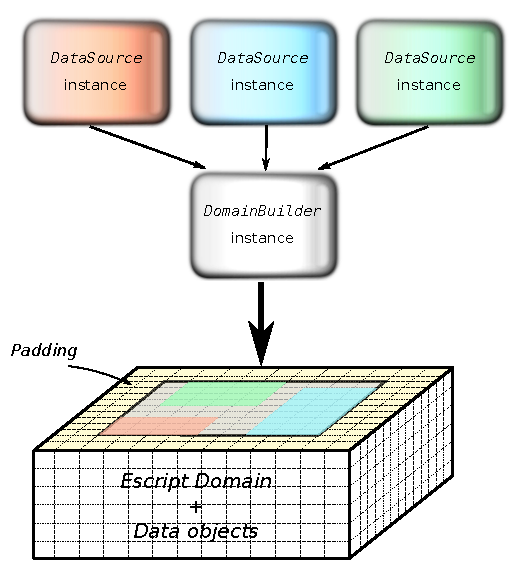
\includegraphics{domainbuilder}
    \caption{\class{DataSource} instances are added to a \class{DomainBuilder}
        which creates a suitable domain and \Data objects for the inversion}
    \label{fig:domainBuilder}
\end{figure}
%
Notice that in the figure there are cells in the region of interest that are
not covered by any data source instance.
Ideally, all data sources used for an inversion have the same spatial resolution
and are spatially adjacent so that all cells have a value but this is not a
requirement.


\section{Domain Builder}\label{Chp:ref:domain builder}
Every inversion requires one \class{DomainBuilder} instance which creates and
holds a reference to the \escript domain as well as associated \Data objects for
the input data used for the inversion.
The class has the following public methods:

\begin{classdesc}{DomainBuilder}{\optional{dim=3, }\optional{reference_system=\None}}
Constructor for the domain builder. \member{dim} sets the dimensionality of the
target domain and must be 2 or 3. By default a 3-dimensional domain is created.
\member{reference_system} defines the reference coordinate system to be used, see Section~\ref{sec:ref:reference systems}.
If not present the Cartesian reference coordinate system is used.
\end{classdesc}

\begin{methoddesc}[DomainBuilder]{addSource}{source}
adds survey data \member{source} (a \class{DataSource} object) to the domain
builder. The dimensionality of the data must be less than or equal to the
domain dimensionality. The reference coordinate system of the \class{DataSource}
must match the reference coordinate system of this class. 
The \member{source} must be defined for the same reference coordinate system to be used, see Section~\ref{sec:ref:reference systems}.
\end{methoddesc}

\begin{methoddesc}[DomainBuilder]{setVerticalExtents}{%
\optional{depth=40000.}%
\optional{, air_layer=10000.}%
\optional{, num_cells=25}}
sets the parameters for the vertical dimension of the domain. The parameter
\member{depth} specifies the thickness in meters of the subsurface layer
($-x_2^{min}$ in Figure~\ref{fig:cartesianDomain}).
The default value of $40$ km is usually appropriate. Similarly, the
\member{air_layer} parameter defines the buffer zone thickness above the surface
($x_2^{max}$ in Figure~\ref{fig:cartesianDomain}) which should be a few
kilometres to avoid artefacts in the inversion.
The number of elements (or cells) in the vertical dimension is set with the
\member{num_cells} parameter. Consider the size and resolution of your datasets,
the total vertical length (=\member{depth}+\member{air_layer}) and available
compute resources when setting this value.
\end{methoddesc}

\begin{methoddesc}[DomainBuilder]{setFractionalPadding}{%
\optional{pad_x=\None}%
\optional{, pad_y=\None}}
sets the amount of padding around the dataset as a fraction of the dataset side
lengths if the reference coordinate system is Cartesian. 
For example, calling \member{setFractionalPadding(0.2, 0.1)} with a data source
of size $10000 \times 20000$ meters will result in the padded data set size $14000 \times 24000$ meters
(that is $10000 \times (1+2 \times 0.2)$ and $20000 \times (1+2 \times 0.1)$).
By default no padding is applied and \member{pad_y} is ignored for 2-dimensional
domains.
\end{methoddesc}

\begin{methoddesc}[DomainBuilder]{setFractionalPadding}{%
\optional{pad_lat=\None}%
\optional{, pad_lon=\None}}
sets the amount of padding around the dataset as a fraction of the dataset side
lengths if the reference coordinate system is not Cartesian.
For example, calling \member{setFractionalPadding(0.2, 0.1)} with a data source
of size $10 \times 20$ degree will result in the padded data set size $14 \times 24$ degree
(that is $10 \times (1+2 \times 0.2)$ and $20 \times (1+2 \times 0.1)$).
By default no padding is applied and \member{pad_lon} is ignored for 2-dimensional
domains.
\end{methoddesc}

\begin{methoddesc}[DomainBuilder]{setPadding}{%
\optional{pad_x=\None}%
\optional{, pad_y=\None}}
sets the amount of padding around the dataset in absolute length units.
The final domain size will be the length in x (in y) of the dataset plus twice
the value of \member{pad_x} (\member{pad_y}). The arguments must be non-negative.
By default no padding is applied and \member{pad_y} is ignored for 2-dimensional
domains. This function can be used for Cartesian reference coordinate system  only.
\end{methoddesc}

\begin{methoddesc}[DomainBuilder]{setElementPadding}{%
\optional{pad_x=\None}%
\optional{, pad_y=\None}}
sets the amount of padding around the dataset in number of elements (cells),
if the reference coordinate system is Cartesian. 
When the domain is constructed \member{pad_x} (\member{pad_y}) elements are
added on each side of the x- (y-) dimension in case of a Cartesian reference system. The arguments must be non-negative integers.
By default no padding is applied and \member{pad_y} is ignored for 2-dimensional
domains.
\end{methoddesc}

\begin{methoddesc}[DomainBuilder]{setElementPadding}{%
\optional{pad_lat=\None}%
\optional{, pad_lon=\None}}
sets the amount of padding around the dataset in number of elements (cells) if the the reference coordinate system is not Cartesian.
When the domain is constructed \member{pad_lat} (\member{pad_lon}) elements are
added on each side of the latitudinal (longitudinal) dimension. The arguments must be non-negative integers.
By default no padding is applied and \member{pad_lon} is ignored for 2-dimensional
domains.
\end{methoddesc}

\begin{methoddesc}[DomainBuilder]{fixDensityBelow}{%
\optional{depth=\None}}
defines the depth below which the density anomaly is fixed to zero.
This method is only useful for inversions that involve gravity data.
\end{methoddesc}

\begin{methoddesc}[DomainBuilder]{fixSusceptibilityBelow}{%
\optional{depth=\None}}
defines the depth below which the susceptibility anomaly is fixed to zero.
This method is only useful for inversions that involve magnetic data.
\end{methoddesc}

\begin{methoddesc}[DomainBuilder]{getGravitySurveys}{}
returns a list of all gravity surveys added to the domain builder. See
\member{getSurveys()} for more details.
\end{methoddesc}

\begin{methoddesc}[DomainBuilder]{getMagneticSurveys}{}
returns a list of all magnetic surveys added to the domain builder. See
\member{getSurveys()} for more details.
\end{methoddesc}

\begin{methoddesc}[DomainBuilder]{getSurveys}{datatype}
returns a list of surveys of type \member{datatype} available to this domain
builder. In the current implementation each survey is a tuple of two \Data
objects, the first containing anomaly values and the second standard error
values for the survey.
\end{methoddesc}

\begin{methoddesc}[DomainBuilder]{getDomain}{}
returns an \escript domain (see~\cite{ESCRIPT}) suitable for running inversions
on the attached data sources.
The first time this method is called the target parameters (such as resolution,
extents and number of elements) are computed, and the domain is created.
Subsequent calls return the same domain instance so calls to
\member{setPadding()}, \member{addSource()} and other methods that influence
the domain will fail once \member{getDomain()} is called the first time.
\end{methoddesc}

\begin{methoddesc}[DomainBuilder]{getReferenceSystem}{}
returns the reference coordinate system
\end{methoddesc}

\begin{methoddesc}[DomainBuilder]{setBackgroundMagneticFluxDensity}{B}
sets the background magnetic flux density $B=(B_{North},B_{East},B_{Vertical})$
which is required for magnetic inversions.
$B_{East}$ is ignored for 2-dimensional magnetic inversions.
\end{methoddesc}

\begin{methoddesc}[DomainBuilder]{getBackgroundMagneticFluxDensity}{}
returns the background magnetic flux density $B$ set via
\member{setBackgroundMagneticFluxDensity()} in a form suitable for the inversion.
There should be no need to call this method directly.
\end{methoddesc}

\begin{methoddesc}[DomainBuilder]{getSetDensityMask}{}
returns the density mask \Data object which is non-zero for cells that have a
fixed density value, zero otherwise.
There should be no need to call this method directly.
\end{methoddesc}

\begin{methoddesc}[DomainBuilder]{getSetSusceptibilityMask}{}
returns the susceptibility mask \Data object which is non-zero for cells that
have a fixed susceptibility value, zero otherwise.
There should be no need to call this method directly.
\end{methoddesc}

\section{\class{DataSource} Class}\label{sec:ref:DataSource}

Data sources added to a \class{DomainBuilder} must provide an implementation for
a few methods as described in the class template \class{DataSource} from
the \module{esys.downunder.datasources} module:

\begin{classdesc}{DataSource}{\optional{reference_system=\None}}
Base constructor which initializes members and should therefore be invoked by
subclasses. Subclasses may then use the member \member{logger} to print any
output. \member{reference_system} defines the reference coordinate system to be used, see Section~\ref{sec:ref:reference systems}.
If not present the Cartesian reference coordinate system is used.
\end{classdesc}

\begin{methoddesc}[DataSource]{getDataExtents}{}
This method should be implemented to return a tuple of tuples
( (x0, y0), (nx, ny), (dx, dy) ), where (x0, y0) denote the UTM coordinates of
the data origin, (nx, ny) the number of data points, and (dx, dy) the spacing
of data points in a Cartesian reference system is used. Otherwise 
the data origin and the spacing refer to latitudinal and longitudinal coordinates.
\end{methoddesc}

\begin{methoddesc}[DataSource]{getDataType}{}
Subclasses must return \class{DataSource}.\member{GRAVITY} or
\class{DataSource}.\member{MAGNETIC} depending on the type of data they provide.
\end{methoddesc}

\begin{methoddesc}[DataSource]{getSurveyData}{domain, origin, NE, spacing}
This method is called by the \class{DomainBuilder} to retrieve the actual survey
data in the form of \Data objects on the \member{domain}.
Data sources are responsible to map or interpolate their data onto the domain
which has been constructed to fit the data.
The domain \member{origin}, number of elements \member{NE} and element
\member{spacing} are provided as tuples or lists to aid with interpolation.
\end{methoddesc}

\begin{methoddesc}[DataSource]{getUtmZone}{}
Must be implemented to return the UTM zone that corresponds to the location of
this data set as returned by \member{getDataExtents}.
\end{methoddesc}

\begin{methoddesc}[DataSource]{setSubsamplingFactor}{factor}
Notifies the data source that data should be subsampled by \member{factor}.
This method does not need to be overwritten.
See \member{getSubsamplingFactor()} for an explanation.
\end{methoddesc}

\begin{methoddesc}[DataSource]{getSubsamplingFactor}{}
Returns the subsampling factor which was set by \member{setSubsamplingFactor()}
or $1$ which indicates that no subsampling is requested.
Data sources that support subsampling (or interleaving) of their data should use
this method to query the subsampling factor before returning surveys via
\member{getSurveyData}. If supported, the factor should be applied in all
dimensions. For example, a 2-dimensional dataset with 300 x 150 data points
should be reduced to 150 x 75 data points when the subsampling factor equals $2$.
Subsampling becomes important when the survey data resolution is too fine or
when using data with varying resolution in one inversion.
Note that data sources may choose to ignore the subsampling factor if they
don't support it.
\end{methoddesc}

\begin{methoddesc}[DataSource]{getReferenceSystem}{}
returns the reference coordinate system
\end{methoddesc}

\vspace{1em}\noindent The \module{esys.downunder.datasources} module contains the following helper
functions:

\begin{funcdesc}{LatLonToUTM}{longitude, latitude%
\optional{, wkt_string=\None}}
converts one or more (longitude,latitude) pairs to the corresponding (x,y)
coordinates in the \emph{Universal Transverse Mercator} (UTM) projection.
This function requires the \module{pyproj} module for conversion and the
\module{gdal} module to parse the \member{wkt_string} parameter if supplied.
The \member{wkt_string} parameter may describe the coordinate system used
for the input values as a \emph{Well-known Text} (WKT) string.
\end{funcdesc}

\subsection{ER Mapper Raster Data}\label{sec:ref:DataSource:ERM}
\emph{ER Mapper} files that contain 2-dimensional raster data may be used for
inversions through the \class{ErMapperData} class which is derived from
\class{DataSource}. Date are given in latitudinal and longitudinal coordinates and if
a Cartesian reference coordinate system is used are mapped using the appropriate  (UTM) projection. 
Generally, these datasets contain two files~\cite{ERMAPPER}, a header file and a data file.
The former usually has the \texttt{.ers} file extension and is a text file that
describes the data format, size, coordinate system used etc.
The data file usually has the same file name but no extension.
Note, that the current implementation may not work with all \emph{ER Mapper}
datasets. For example, the only cell type understood is \emph{IEEE4ByteReal}
at the moment.
To run inversions on a \emph{ER Mapper} dataset use the following constructor:
\begin{classdesc}{ErMapperData}{data_type, headerfile%
\optional{, datafile=\None}%
\optional{, altitude=0.}%
\optional{, error=\None}%
\optional{, scale_factor=\None}%
\optional{, null_value=\None}
\optional{, reference_system=\None}}
Creates a new data source from \emph{ER Mapper} data.
The parameter \member{data_type} must be one of
\class{DataSource}.\member{GRAVITY} or \class{DataSource}.\member{MAGNETIC}
depending on the type of data, \member{headerfile} is the name of the header
file while \member{datafile} specifies the name of the data file.
The parameter \member{datafile} can be left blank if the name is identical to
the header file except for the file extension.
The \member{altitude} parameter can be used to shift a 2-dimensional slice of
data vertically within a 3-dimensional domain.
Use \member{error} to set the (constant) measurement error with the same units
used by the measurements. By default a value of $2$ units is assumed which
equals $0.2 \; mgal$ or $2 \; nT$ depending on the data type.
Since ER Mapper files do not store any information about data units or scale
the \member{scale_factor} may be used to provide this information.
If not set, gravity data is assumed to be given in $\frac{\mu m}{sec^2}$ while
magnetic data is assumed to be given in $nT$.
Finally, the \member{null_value} parameter can be used to override the value
for the areas to be ignored (see Section~\ref{SEC:P1:GRAV:REMARK:DATAHOLES})
which is usually provided in the ER Mapper header file.
\member{reference_system} defines the reference coordinate system to be used, see Section~\ref{sec:ref:reference systems}.
If not present the Cartesian reference coordinate system is used. In the current implementation any
coordinate system specified in the file is ignored.
\end{classdesc}

\subsection{NetCDF Data}\label{sec:ref:DataSource:NETCDF}
The \class{NetCdfData} class from the \module{esys.downunder.datasources} module
provides the means to use data from \netcdf files~\cite{NETCDF} for inversion.
Currently, files that follow the \emph{Climate and Forecast (CF)}\footnote{%
\url{http://cf-pcmdi.llnl.gov/documents/cf-conventions/latest-cf-conventions-document-1}}
and/or the \emph{Cooperative Ocean/Atmosphere Research Data Service (COARDS)}\footnote{%
\url{http://ferret.wrc.noaa.gov/noaa_coop/coop_cdf_profile.html}} metadata
conventions are supported.
The example script \examplefile{create_netcdf.py} demonstrates how a compatible
file can be generated from within \Python (provided the \module{scipy} module
is available).
To plot such an input file including coordinates and legend using
\emph{matplotlib}~\cite{matplotlib} see the script \examplefile{show_netcdf.py}.
The interface to \class{NetCdfData} looks as follows:

\begin{classdesc}{NetCdfData}{datatype, filename%
\optional{, altitude=0.}%
\optional{, data_variable=\None}%
\optional{, error=\None}%
\optional{, scale_factor=\None}%
\optional{, null_value=\None}
\optional{, reference_system=\None}}
Creates a new data source from compatible \netcdf data.
The two required parameters are \member{datatype}, which must be one of
\class{DataSource}.\member{GRAVITY} or \class{DataSource}.\member{MAGNETIC}
depending on the type of data, and \member{filename} which is the name of the
file containing the data.
The \member{altitude} parameter can be used to shift a 2-dimensional slice of
data vertically within a 3-dimensional domain.
Set the \member{data_variable} parameter to the name of the \netcdf variable
that contains the measurements unless there is only one data variable in the
file in which case the parameter can be left empty.
Use \member{error} to set the (constant) measurement error with the same units
used by the measurements or the name of the \netcdf variable that contains this
information. By default a value of $2$ units is assumed which equals
$0.2 \; mgal$ or $2 \; nT$ depending on the data type.
The current implementation does not use the units attribute (if available)
within the \netcdf file. Use the \member{scale_factor} argument to provide this
information instead.
If not set, gravity data is assumed to be given in $\frac{\mu m}{sec^2}$ while
magnetic data is assumed to be given in $nT$.
Finally, the \member{null_value} parameter can be used to override the value
for the areas to be ignored (see Section~\ref{SEC:P1:GRAV:REMARK:DATAHOLES})
which is usually provided in the \netcdf file. \member{reference_system} defines the reference coordinate system to be used, see Section~\ref{sec:ref:reference systems}.
If not present the Cartesian reference coordinate system is used. In the current implementation any
coordinate system specified in the file is ignored.
\end{classdesc}

\subsection{Synthetic Data}
As a special case the \module{esys.downunder.datasources} module contains
classes to generate input data for inversions by solving a forward model with
user-defined reference data.
The main purpose of using synthetic data is to test the capabilities of the
inversion module or for tracking down problems.

The base class for synthetic data which is derived from \class{DataSource}
has the following interface:

\begin{classdesc}{SyntheticDataBase}{datatype%
\optional{, DIM=2}
\optional{, number_of_elements=10}
\optional{, length=1*U.km}def SphericalReferenceSystem(R=6378137.0*U.m):
\optional{, B_b=\None}
\optional{, data_offset=0}
\optional{, full_knowledge=\False}}
Base class to define reference data based on a given property distribution
(density or susceptibility). Data are collected from a square region of
vertical extent \member{length} on a grid with \member{number_of_elements}
cells in each direction.
The synthetic data are constructed by solving the appropriate forward problem.
Data can be sampled with an offset from the surface at $z=0$ or using the
entire subsurface region.
\end{classdesc}

\vspace{1em}\noindent The only additional method which needs to be implemented
in subclasses is
\begin{methoddesc}[SyntheticDataBase]{getReferenceProperty}{
\optional{domain=\None}}
Returns the reference \Data object that was used to generate the gravity or
susceptibility anomaly data. The \member{domain} argument must be present
when this method is called for the first time but not necessarily in
subsequent calls.
\end{methoddesc}

\vspace{1em}\noindent Two synthetic data providers are currently available.
The class \class{SyntheticData} defines synthetic gravity or magnetic anomaly
data based on a harmonic
\begin{equation}\label{eq:synthdata}
    k=A\cdot sin\left(\pi \frac{n_D}{D} (z+\Delta z)\right) \cdot%
        sin\left(\pi \frac{n_L}{L} (x - x_0)\right)
\end{equation}
where $A$ is the amplitude, $n_D$, $n_L$ denote the number of oscillations in
the vertical and lateral direction, respectively, while $D$ and $L$ is the
depth and side length for the data, respectively.
The second data provider class is \class{SyntheticFeatureData} which takes a
list of \class{SourceFeature} objects that define the anomaly and is thus more
generic.
The constructors are defined as follows:

\begin{classdesc}{SyntheticData}{datatype%
\optional{, n_length=1}
\optional{, n_depth=1}
\optional{, depth_offset=0.}
\optional{, depth=\None}
\optional{, amplitude=\None}
\optional{, DIM=2}
\optional{, number_of_elements=10}
\optional{, length=1*U.km}
\optional{, B_b=\None}
\optional{, data_offset=0}
\optional{, full_knowledge=\False}
\optional{, spherical=\False}}
The arguments \member{n_length}, \member{n_depth}, \member{depth_offset},
\member{depth}, and \member{amplitude} correspond to the respective symbols in
Equation~\ref{eq:synthdata}. The remaining arguments are passed to the parent
class (\class{SyntheticDataBase}) and described there.
If \member{depth} is not set the depth of the domain is used.
The argument \member{amplitude} may be left unset as well in which case a
default value is used ($200 \frac{kg}{m^3}$ for gravity and $0.1$ for magnetic
data).
\end{classdesc}

\begin{classdesc}{SyntheticFeatureData}{datatype, features%
\optional{, DIM=2}
\optional{, number_of_elements=10}
\optional{, length=1*U.km}
\optional{, B_b=\None}
\optional{, data_offset=0}
\optional{, full_knowledge=\False}
\optional{, spherical=\False}}
The only new argument is \member{features} which is a list of
\class{SourceFeature} objects to be included in the data preparation.
All other arguments are passed on to the parent class (see there).
\end{classdesc}

\begin{classdesc}{SourceFeature}{}
A feature adds a density/susceptibility distribution to (parts of) a domain of
a synthetic data source, for example a layer of a specific rock type or a
simulated ore body. This base class is empty and only provides the skeleton
for subclasses which need to implement the following two methods:
\end{classdesc}

\begin{methoddesc}[SourceFeature]{getValue}{}
Returns the value for the area covered by mask. It can be constant or a \Data
object with spatial dependency.
\end{methoddesc}

\begin{methoddesc}[SourceFeature]{getMask}{x}
Returns the mask of the region of interest for this feature. That is, mask is
non-zero where the value returned by \member{getValue()} should be applied,
zero elsewhere.
\end{methoddesc}


\chapter{Regularization}\label{Chp:ref:regularization}

The general cost function $J^{total}$ to be minimized has some of the cost
function $J^f$ measuring the defect of the result from the
forward model with the data, and the cost function $J^{reg}$ introducing the
regularization into the problem and makes sure that a unique answer exists.
The regularization term is a function of, possibly vector-valued, level set
function $m$ which represents the physical properties to be represented and is,
from a mathematical point of view, the unknown of the inversion problem.
It is the intention that the values of $m$ are between zero and one and that
actual physical values are created from a mapping before being fed into a
forward model. In general the cost function $J^{reg}$ is defined as 
\begin{equation}\label{EQU:REG:1}
J^{reg}(m) = \frac{1}{2} \int_{\Omega} \left(
 \sum_{k} \mu_k \cdot ( \omega^{(0)}_k \cdot m_k^2 + \omega^{(1)}_{ki}m_{k,i}^2 ) 
+  \sum_{l<k} \mu^{(c)}_{lk} \cdot \omega^{(c)}_{lk}  \cdot  \chi(m_l,m_k) \right) \; dx 
\end{equation} 
where summation over $i$ is performed. The additional trade--off factors 
$\mu_k$ and $\mu^{(c)}_{lk}$ ($l<k$) are between zero and one and constant across the 
domain. They are potentially modified during the inversion in order to improve the balance between the different terms 
in the cost function.

$\chi$ is a given symmetric, non-negative cross-gradient function\index{cross-gradient
}. We use
\begin{equation}\label{EQU:REG:4}
 \chi(a,b) =  ( a_{,i} a_{,i}) \cdot ( b_{,j} b_{,j}) -   ( a_{,i} b_{,i})^2 
\end{equation} 
where summations over $i$ and $j$  are performed. Notice that cross-gradient function
is measuring the angle between the surface normals of contours of level set functions. So 
minimizing the cost function will align the surface normals of the contours.

The coefficients $\omega^{(0)}_k$, $\omega^{(1)}_{ki}$ and $\omega^{(c)}_{lk}$ define weighting factors which 
may depend on their location within the domain. We assume that for given level set function $k$ the 
weighting factors $\omega^{(0)}_k$, $\omega^{(1)}_{ki}$ are scaled such that 
\begin{equation}\label{ref:EQU:REG:5}
\int_{\Omega} ( \omega^{(0)}_k  + \frac{\omega^{(1)}_{ki}}{L_i^2} ) \; dx = \alpha_k 
\end{equation} 
where $\alpha_k$ defines the scale which is typically set to one. $L_i$ is the width of the domain in $x_i$ direction.
Similarly we set for $l<k$ we set 
\begin{equation}\label{ref:EQU:REG:6}
\int_{\Omega} \frac{\omega^{(c)}_{lk}}{L^4} \; dx = \alpha^{(c)}_{lk}
\end{equation} 
where $\alpha^{(c)}_{lk}$ defines the scale which is typically set to one and
\begin{equation}\label{ref:EQU:REG:6b}
\frac{1}{L^2} = \sum_i \frac{1}{L_i^2} \;.
\end{equation} 

In some cases values for the level set functions are known to be zero at certain regions in the domain. Typically this is the region 
above the surface of the Earths. This expressed using a
a characteristic function $q$ which varies with its location within the domain. The function $q$ is set to zero except for those 
locations $x$ within the domain where the values of the level set functions is known to be zero. For these locations $x$
$q$ takes a positive value. for a single level set function one has
\begin{equation}\label{ref:EQU:REG:7}
q(x) = \left\{ 
\begin{array}{rl}
  1 & \mbox{ if } m \mbox{ is set to zero at location } x \\
  0 & \mbox{ otherwise }
\end{array}
\right.
\end{equation} 
For multi-valued level set function the  characteristic function is set componentwise:
\begin{equation}\label{ref:EQU:REG:7b}
q_k(x) = \left\{ 
\begin{array}{rl}
  1 & \mbox{ if component } m_k \mbox{ is set to zero at location } x \\
  0 & \mbox{ otherwise }
\end{array}
\right.
\end{equation} 


\section{Usage}

\LG{Add example}

\begin{classdesc}{Regularization}{domain
        \optional{, w0=\None}
        \optional{, w1=\None}
        \optional{, wc=\None}
        \optional{, location_of_set_m=Data()}
        \optional{, numLevelSets=1}
        \optional{, useDiagonalHessianApproximation=\False}
        \optional{, tol=1e-8}
        \optional{, scale=\None}
        \optional{, scale_c=\None}
        }

  
initializes a regularization component of the cost function for inversion. 
\member{domain} defines the domain of the inversion. \member{numLevelSets}
sets the number of level set functions to be found during the inversion. 
\member{w0}, \member{w1} and  \member{wc} define the weighting factors
$\omega^{(0)}$,
$\omega^{(1)}$ and
$\omega^{(c)}$, respectively. A value for \member{w0} or \member{w1} or both must be given. 
If more then one level set function is involved  \member{wc} must be given. 
\member{location_of_set_m} sets the characteristic function $q$ 
to define locations where the level set function is set to zero, see equation~(\ref{ref:EQU:REG:7}).
\member{scale} and 
\member{scale_c} set the scales $\alpha_k$ in equation~(\ref{ref:EQU:REG:5}) and
$\alpha^{(c)}_{lk}$ in equation~(\ref{ref:EQU:REG:6}), respectively. By default, their values are set to one.
Notice that weighting factors are rescaled to meet the scaling conditions. \member{tol} sets the 
tolerance for the calculation of the Hessian approximation. \member{useDiagonalHessianApproximation} 
indicates to ignore coupling in the Hessian approximation produced by the 
cross-gradient term. This can speed-up an individual iteration step in the inversion but typically leads to more
inversion steps.
\end{classdesc}

\section{Gradient Calculation}


The cost function kernel\index{cost function!kernel} is given as
\begin{equation}\label{ref:EQU:REG:100}
K^{reg}(m) = \frac{1}{2}
\sum_{k} \mu_k \cdot ( \omega^{(0)}_k \cdot m_k^2 + \omega^{(1)}_{ki}m_{k,i}^2 ) 
+  \sum_{l<k} \mu^{(c)}_{lk} \cdot \omega^{(c)}_{lk}  \cdot  \chi(m_l,m_k)
\end{equation} 
We need to provide the gradient of the cost function $J^{reg}$  with respect to the level set functions $m$.
The gradient is represented by two functions $Y$ and $X$ which define the 
derivative of the cost function kernel with respect to $m$ and to the gradient $m_{,i}$, respectively:
\begin{equation}\label{ref:EQU:REG:101}
\begin{array}{rcl}
  Y_k & = & \displaystyle{\frac{\partial K^{reg}}{\partial m_k}} \\
   X_{ki} & = & \displaystyle{\frac{\partial K^{reg}}{\partial m_{k,i}}} 
\end{array}
\end{equation} 
For the case of a single valued level set function $m$ we get 
\begin{equation}\label{ref:EQU:REG:202}
Y = \mu \cdot \omega^{(0)} \cdot m
\end{equation} 
and 
\begin{equation}\label{ref:EQU:REG:203}
 X_{i} = \mu \cdot \omega^{(1)}_{i} \cdot m_{,i}
\end{equation}
For a two-valued level set function $(m_0,m_1)$ we have
\begin{equation}\label{ref:EQU:REG:302}
Y_k = \mu_k \cdot \omega^{(0)}_k \cdot m_k \mbox{ for } k=0,1
\end{equation} 
and for $X$ 
\begin{equation}\label{ref:EQU:REG:303}
\begin{array}{rcl}
 X_{0i} &  = & \mu_0 \cdot \omega^{(1)}_{0i} \cdot m_{0,i} + \mu^{(c)}_{01} \cdot \omega^{(c)}_{01} \cdot
\left( (m_{1,j}m_{1,j} ) \cdot m_{0,i} - (m_{1,j}m_{0,j} ) \cdot m_{1,i} \right) \\
 X_{1i} &  = & \mu_1 \cdot \omega^{(1)}_{1i} \cdot m_{1,i} + \mu^{(c)}_{01} \cdot \omega^{(c)}_{01} \cdot
\left( (m_{0,j}m_{0,j} ) \cdot m_{1,i} - (m_{1,j}m_{0,j} ) \cdot m_{0,i} \right)
\\
\end{array}
\end{equation}  
We also need to provide an approximation of the inverse of the Hessian operator. The operator evaluation is executes as a solution 
of a linear PDE which is solved using \escript \class{LinearPDE} class. In the \escript notation we need to provide 
\begin{equation}\label{ref:EQU:REG:600}
\begin{array}{rcl}
 A_{kilj} & = & \displaystyle{\frac{\partial X_{ki}}{\partial m_{l,j}}} \\
D_{kl} & =  &  \displaystyle{\frac{\partial Y_{k}}{\partial m_{l}}} 
\end{array}
\end{equation} 
For the case of a single valued level set function $m$ we get 
\begin{equation}\label{ref:EQU:REG:601}
\begin{array}{rcl}
 A_{ij} & =&  \mu \cdot \omega^{(1)}_i \cdot \delta_{ij}  \\
D & = &  \mu \cdot \omega^{(0)} 
\end{array}
\end{equation}
For a two-valued level set function $(m_0,m_1)$ we have
\begin{equation}\label{ref:EQU:REG:602}
D_{kl}  =   \mu_k \cdot \omega^{(0)}_k \cdot \delta_{kl} 
\end{equation} 
and 
\begin{equation}\label{ref:EQU:REG:603}
\begin{array}{rcl}
A_{0i0j} & = & \mu_0 \cdot \omega^{(1)}_{0i} \cdot \delta_{ij} + \mu^{(c)}_{01} \cdot \omega^{(c)}_{01} \cdot 
\left( (m_{1,j'}m_{1,j'} )\cdot \delta_{ij}  -  m_{1,i} \cdot m_{1,j} \right)    \\
A_{0i1j} & = & \mu^{(c)}_{01} \cdot \omega^{(c)}_{01} \cdot \left( 2 \cdot m_{0,i} \cdot  m_{1,j}
- m_{1,i} \cdot  m_{0,j} - ( m_{1,j'} m_{0,j'} ) \cdot  \delta_{ij}
\right)  \\
A_{1i0j} & = & \mu^{(c)}_{01} \cdot \omega^{(c)}_{01} \cdot \left( 2 \cdot m_{1,i} \cdot  m_{0,j}
- m_{0,i} \cdot  m_{1,j} - ( m_{1,j'} m_{0,j'} ) \cdot  \delta_{ij} \right)  \\
A_{1i1j} & = &  \mu_1 \cdot \omega^{(1)}_{1i} \cdot \delta_{ij} + \mu^{(c)}_{01} \cdot \omega^{(c)}_{01} \cdot
\left( (m_{0,j'}m_{0,j'} ) \cdot \delta_{ij}  -  m_{0,i} \cdot m_{0,j}  ) \right) 
\end{array}
\end{equation} 



\chapter{Mapping}\label{Chp:ref:mapping}

Mapping classes map a level set function $m$ as described in Chapter~\ref{Chp:ref:regularization}
onto a physical parameter such as density and susceptibility. 

\section{Density Map}\label{Chp:ref:mapping density}
For density we use the form 
\begin{equation}\label{EQU:MAP:1}
\rho =  \rho_{0} + \Delta \rho \cdot \left( \frac{x_2 - z_0}{l_z} \right)^{\frac{\beta}{2}}  \cdot m 
\end{equation}  
where $\rho_{0}$ is the reference density, $\Delta \rho$ is the density scaling, $z_0$ an offset, $l_z$ vertical expansion
of the domain and $\beta$ is a suitable exponent. 

\begin{classdesc}{DensityMapping}{domain
        \optional{, z0=None}
        \optional{, rho0=0}
        \optional{, drho=$2750 \cdot kg \cdot m^{-3}$}
        \optional{, beta=2.}}
a linear density mapping including depth weighting. \member{domain} is the
domain of the inversion, \member{z0} reference depth in the depth weighting
factor, \member{drho} is the density scaling factor (by default the density of
granite is used) and \member{beta} is the exponent in the depth weighting factor.
If no reference depth \member{z0} is given no depth weighting is applied.
\member{rho0} is the reference density which may be a function of its location
in the domain. 
\end{classdesc}

\begin{methoddesc}[DensityMapping]{getValue}{m}
returns the density for level set function $m$
\end{methoddesc}

\begin{methoddesc}[DensityMapping]{getDerivative}{m}
return the derivative of density  with respect to the level set function.
\end{methoddesc}  

\begin{methoddesc}[DensityMapping]{getInverse}{p}
returns the value level set function $m$ for given density value $p$.
\end{methoddesc}


\section{Susceptibility Map}\label{Chp:ref:mapping susceptibility}
For the magnetic susceptibility $k$ the following mapping is used:
\begin{equation}\label{EQU:MAP:2}
k=  k_{0} + \Delta k \cdot \left( \frac{x_2 - z_0}{l_z} \right)^{\frac{\beta}{2}}  \cdot m 
\end{equation}  
where $k_{0}$ is the reference density and $\Delta k$ is the density scaling.

\begin{classdesc}{SusceptibilityMapping}{domain
        \optional{, z0=None}
        \optional{, k0=0}
        \optional{, dk=1}
        \optional{, beta=2.}}
a linear susceptibility mapping including depth weighting.
\member{domain} is the domain of the inversion, \member{z0} reference depth in
the depth weighting factor, \member{dk} is the susceptibility scaling factor
(by default one is used) and \member{beta} is the exponent in the depth
weighting factor. If no reference depth \member{z0} is given no depth
weighting is applied.
\member{k0} is the reference susceptibility which may be a function of its
location in the domain. 
\end{classdesc}

\begin{methoddesc}[SusceptibilityMapping]{getValue}{m}
returns the susceptibility for level set function $m$
\end{methoddesc}

\begin{methoddesc}[SusceptibilityMapping]{getDerivative}{m}
return the derivative of susceptibility  with respect to the level set function.
\end{methoddesc}  

\begin{methoddesc}[SusceptibilityMapping]{getInverse}{p}
returns the value level set function $m$ for given susceptibility value $p$.
\end{methoddesc}


\section{General Mapping}
Users can define their own mapping $p=\Psi(m)$.
The following interface needs to be served

\begin{classdesc}{Mapping}{}
mapping of a level set function onto a physical parameter to be used by a
forward model.
\end{classdesc} 

\begin{methoddesc}[Mapping]{getValue}{m}
returns the result $\Psi(m)$ of the mapping for level set function $m$
\end{methoddesc}

\begin{methoddesc}[Mapping]{getDerivative}{m}
return the derivative $\frac{\partial \Psi}{\partial m}$ of the mapping with respect to the level set function for 
the level set function $m$.
\end{methoddesc}  

\begin{methoddesc}[Mapping]{getInverse}{p}
returns the value level set function $m$ for given value $p$ of the physical parameter, ie $p=\Psi(m)$.  
\end{methoddesc}



\chapter{Forward Models}\label{Chp:ref:forward models}


%%%%%%%%%%%%%%%%%%%%%%%%%%%%%%%%%%%%%%%%%%%%%%%%%%%%%%%%%%%%%%%%%%%%%%%%%%%%%%
% Copyright (c) 2003-2012 by University of Queensland
% http://www.uq.edu.au
%
% Primary Business: Queensland, Australia
% Licensed under the Open Software License version 3.0
% http://www.opensource.org/licenses/osl-3.0.php
%
% Development until 2012 by Earth Systems Science Computational Center (ESSCC)
% Development since 2012 by School of Earth Sciences
%
%%%%%%%%%%%%%%%%%%%%%%%%%%%%%%%%%%%%%%%%%%%%%%%%%%%%%%%%%%%%%%%%%%%%%%%%%%%%%%

\section{Gravity Inversion}\label{sec:forward gravity}


If the density field $\rho$ is known the gravitational potential $\psi$ is given
as the solution of the PDE 
\begin{equation}\label{GRAV:EQU:100}
\psi_{,ii} = 4\pi \cdot G \cdot  \rho
\end{equation}
where $G=6.67300 \cdot 10^{-11}  \frac{m^3}{kg \cdot s^2}$ is the gravitational constant.  
The gravity force $g_i$ is given
as the negative of the gradient of the gravity potential $\psi$:
\begin{equation}\label{GRAV:EQU:101}
 g_i = - \psi_{,i} 
\end{equation} 
The boundary conditions for PDE~\ref{GRAV:EQU:100} are set as follows:
On vertical faces of the domain we assume that the horizontal gravity forces are equal to zero:
\begin{equation}\label{GRAV:EQU:101a}
\begin{array}{ll}
g_0=0 & \mbox{ for } x_0=x^{min}_0 \mbox{ or } x_0=x^{max}_0 \\
g_1=0 & \mbox{ for } x_1=x^{min}_1 \mbox{ or } x_1=x^{max}_1 \\
\end{array}
\end{equation}
which translates to
\begin{equation}\label{GRAV:EQU:101aa}
n_i \cdot  \psi_{,i} = 0
\end{equation} 
on faces $x_0=x^{min}_0$, 
$x_0=x^{max}_0$,
$x_1=x^{min}_1$ or 
$x_1=x^{max}_1$. On the bottom surface we set 
\begin{equation}\label{GRAV:EQU:101b}
\psi = 0 \mbox{ for } x_2=x^{min}_2
\end{equation} 
which sets all horizontal gravity forces to zero $g_0=g_1=0$. 
For the boundary conditions on the top surface we consider two options
\begin{itemize}
 \item[(D)] 
On the top surface we set 
\begin{equation}\label{GRAV:EQU:101 BC D}
\psi = 0 \mbox{ for } x_2=x^{max}_2
\end{equation} 
which sets all horizontal gravity forces to zero $g_0=g_1=0$.
 \item[(N)] 
On the top surface we set the vertical gravity forces to zero:
\begin{equation}\label{GRAV:EQU:101 BC N}
n_i \cdot  \psi_{,i} = 0 \mbox{ for } x_2=x^{max}_2
\end{equation} 
\end{itemize}
The PDE~\ref{GRAV:EQU:100} together with the boundary conditions~\ref{GRAV:EQU:101aa}, ~\ref{GRAV:EQU:101b}
and~\ref{GRAV:EQU:101 BC D} or~\ref{GRAV:EQU:101 BC N}
has a unique solution. For a given density $\rho$ we denote the unique solution $\psi$ by $\Psi[\rho]$.


The problem is to calculate the density distribution $\rho$ from the gravity force known at some parts of the region of interest 
$\Omega$. In fact we want to minimize the value
\begin{equation}\label{GRAV:EQU:102}
J_{data}(\psi) = \frac{1}{2}\sum_{s} \int_{\Omega} \chi^{(s)}_i \cdot (  g_{i}- g^{(s)}_i)^2 dx
\footnote{Summation over $i$ is performed by Einstein notation.}
\end{equation} 
where $g^{(s)}_i$ is a measurement of the gravity force $g_i=-\psi_{,i}$ and $\chi^{(s)}_i$ is a weighting factor. 
$s$ indexes the surveys included in the inversion. 
We assume that the gravity force $g^{(s)}_i$ is measured as deviation from a background gravity force $g^{bg}_i$,
i.e. the actually present gravity force is given as  $g^{(s)}_i + g^{bg}$~\footnote{Notice that we use the same reference gravity force for all surveys.}.
This can be added to the 
gravitational potential $\psi$ 
\begin{equation}\label{GRAV:EQU:102x}
\psi^{total} = \psi + g^{bg}_i \cdot ( x_i - x^{min}_i ) 
\end{equation}
The total gravitational potential $\psi^{total}$ still fulfills the PDE~\ref{GRAV:EQU:100} 
with inhomogeneous versions of the boundary conditions. For the most common case of a purely vertical
background gravity force (i.e. $g^{bg}_0=g^{bg}_1=0$) the boundary conditions at the top of the domain
take the form $\psi^{total} =g^{bg}_2 \cdot ( x_2^{max} - x^{min}_2 )$ for case (D) or
$n_i \cdot  \psi^{total}_{,i} =g^{bg}_2$ for case (N). Notice that the first case does not enforce
the background gravity force on the top surface but enforces the vertical gravity forces to be zero. 
The second condition for case (D) enforces the vertical gravity force to the background gravity force but allows 
for a non-zero vertical gravity force. In most cases the case (N) is the appropriate boundary condition
assuming the top boundary of the domain is sufficiently far away from any density variation.   
 

In field observations  $g^{(s)}_i$
are known on a sub-domain of the domain only so one will set
\begin{equation}\label{GRAV:EQU:105}
\chi^{(s)}_i 
= \left\{
\begin{array}{lcl}
\frac{1}{(\sigma^{(s)}_i)^2} & & g^{(s)}_i \mbox{ is available} \\
& \mbox{ where } & \\
0 & & \mbox{ otherwise } \\
\end{array}
\right.
\end{equation} 
where $\sigma^{(s)}_i$ is the standard error deviation of measurement $g^{(s)}_i$, see~\cite{A}.
With this setting the data $g^{(s)}_i$ can be extended to any arbitrary value (typically to zero) on
all locations where no measurements of $g^{(s)}_i$ are available.  

We need to make sure that the density $\rho$ takes physically meaningful values. 
To achieve this we use a parametrization $C(m)$ for the $\rho$ where $C$ is a given function. We think as 
$m$ being a dimensionless value between $-\infty$ to $\infty$. Possible settings for the function $C$ are:
\begin{itemize}
 \item[(I)] We can set $\rho = C(m)= \rho^{scale} \cdot m$ where $\rho^{scale}$ is a reference density.
 \item[(B)] To restrict the density $\rho$ between 
a minimum density $\rho^{min}$ and a maximum density $\rho^{max}$ one sets 
\begin{equation} 
\rho = C(m) = \frac{\rho^{max} +\rho^{min}}{2} + \frac{\rho^{max} -\rho^{min}}{2} \cdot \tanh(m)
\end{equation} 
 \item[(L)] To use a logarithmic scale which ensures a positive density one sets
\begin{equation} 
\rho = C(m) = \rho^{scale} \cdot e^{m}
\end{equation} 
\end{itemize}
In the following the exact form of the parametrization $C$ is not relevant, however we will make use of the 
fact that $C$ is sufficiently smooth and invertible, i.e. for any given valid density $\rho$ there is a unique
 value $m$ in the parameter space such that $\rho=C(m)$. For the inverse function we use the notation $C^{-1}$.
In the minimization problem we will search for the value of $m$ providing the best fit to the data 
rather than the density $\rho$. 


The regularization term is added into the minimization problem so the problem has a unique answer. This
takes the form 
\begin{equation}\label{GRAV:EQU:104}
J_{reg}(m) =  \int_{\Omega} \omega \cdot (m-m^{ref})^2 + \omega_i \cdot L_i^2 \cdot [ (m -m^{ref})_{,i}] ^2 dx
\end{equation} 
where $\omega$ and $\omega_i$ are weighting factors, $L_i$ is the smoothing length (e.g. $L_i= x^{max}_i-x^{min}_i$)
and $m^{ref}=C^{-1}(\rho^{ref})$ defines a reference parametrization for a given reference 
density $\rho^{ref}$. 
If the density (and therefore the parameter $m$) is known to be exactly $\rho^{ref}$ on a certain subregion $\Omega^{ref}$ of
the domain this information can be used
to directly constraint the problem, or alternatively one can choose the weights $\omega$. 

The task is now to find $m$ which minimizes the cost function
\begin{equation}\label{GRAV:EQU:103}
f(m) =  J_{data}(\Psi[C[m]]) +  \mu \cdot J_{reg}(m)
\end{equation} 
where $\mu>0$ is a fixed penalty factor subject to $m=m^{ref}$ on $\Omega^{ref}$.

\subsection{Solution methods}
To apply the Nonlinear Conjugate Gradient method (NLCG), see Appendix~\ref{sec:NLCG} or the L-BFGS method, see Appendix~\ref{sec:LBFGS} we need
to define an inner product $<.,.>$ and need to calculate the gradient of of $f$. 

As inner product we use 
\begin{equation}\label{GRAV:EQU:200}
<p,q> = \int_{\Omega} p \cdot q \; dx
\end{equation} 
With this notation the gravity potential $\phi$ is given as
\begin{equation}\label{GRAV:EQU:201}
< q_{,i},\psi_{,i} > = - 4\pi \cdot G \cdot  < q , \rho > \mbox{ for all } q \mbox{ with } q=0 \mbox{ on } \Gamma_{z}
\end{equation} 
where $\Gamma_{z}$ denotes the top and bottom surface of the domain for case (D)
and the top surface of the domain for case (N). 


For any $q$ with $q=0$ on $\Omega^{ref}$ we get 
\begin{equation}\label{GRAV:EQU:202}
< \nabla f(m),q> = < \nabla J_{data}(\Psi[C[m]]), q>  +  \mu \cdot < \nabla J_{reg}(m),q>
\end{equation} 
with 
\begin{equation}\label{GRAV:EQU:202a}
< \nabla J_{reg}(m),q> = 
\int_{\Omega} 2 \omega q \cdot (m-m^{ref}) + 2 \omega_i \cdot L_i^2 \cdot q_{,i} (m-m^{ref})_{,i} dx
\end{equation} 
and 
\begin{equation}\label{GRAV:EQU:202b}
< \nabla J_{data}(\Psi[C[m]]), q> = 
\sum_{s} \int_{\Omega} \chi^{(s)}_i \cdot (  \psi_{,i} +  g^{(s)}_i)  \cdot (\Psi[\frac{dC}{dm} \cdot q])_{,i} dx 
\end{equation} 
where $\rho=C(m)$ and $\psi=\Psi[\rho]$. We then set 
\begin{equation}\label{GRAV:EQU:202c}
Z_i[\psi]= \sum_{s} \chi^{(s)}_i \cdot (  \psi_{,i} +  g^{(s)}_i) 
\end{equation} 
and $Z^*[\psi]$ as the solution of the equation 
\begin{equation}\label{GRAV:EQU:202d}
< p_{,i},Z^*[\psi]_{,i} > =  < p_{,i} ,Z_i[\psi] > \mbox{ for all } p \mbox{ with } p=0 \mbox{ on } \Gamma_{z}
\end{equation} 
with $Z^*[\psi]=0$ on $\Gamma_{z}$. By stetting $p=\Psi_0[\frac{dC}{dm} \cdot q]$ we get
\begin{equation}\label{GRAV:EQU:202e}
<(\Psi_0[\frac{dC}{dm} \cdot q]) _{,i},Z^*[\psi]_{,i} > =  < (\Psi_0[\frac{dC}{dm} \cdot q])_{,i} ,Z_i[\psi] >
\end{equation} 
and from~\ref{GRAV:EQU:201} with $q=Z^*[\psi]$ we get
\begin{equation}\label{GRAV:EQU:20e}
< (Z^*[\psi])_{,i},(\Psi_0[\frac{dC}{dm} \cdot q])_{,i} > = - 4\pi \cdot G \cdot  < Z^*[\psi], \frac{dC}{dm} \cdot q >
\end{equation}
which leads to 
\begin{equation}\label{GRAV:EQU:202f}
< \nabla J_{data}(\Psi[C[m]]), q> = < (\Psi_0[\frac{dC}{dm} \cdot q])_{,i} ,Z_i[\psi] > 
=  - 4\pi \cdot G \cdot  < \frac{dC}{dm} Z^*[\psi] , q > 
\end{equation} 
Putting this all together we get
\begin{equation}\label{GRAV:EQU:202g}
< \nabla f(m),q> = 
\mu \cdot < 2 \omega \cdot (m-m^{ref}), q>
+ \mu \cdot < 2 \omega_i \cdot L_i^2 \cdot (m-m^{ref})_{,i}, q_{,i}> - 4\pi \cdot G \cdot  < \frac{dC}{dm} Z^*[\psi] , q > 
\end{equation}  



%%%%%%%%%%%%%%%%%%%%%%%%%%%%%%%%%%%%%%%%%%%%%%%%%%%%%%%%%%%%%%%%%%%%%%%%%%%%%%
% Copyright (c) 2003-2012 by University of Queensland
% http://www.uq.edu.au
%
% Primary Business: Queensland, Australia
% Licensed under the Open Software License version 3.0
% http://www.opensource.org/licenses/osl-3.0.php
%
% Development until 2012 by Earth Systems Science Computational Center (ESSCC)
% Development since 2012 by School of Earth Sciences
%
%%%%%%%%%%%%%%%%%%%%%%%%%%%%%%%%%%%%%%%%%%%%%%%%%%%%%%%%%%%%%%%%%%%%%%%%%%%%%%


\section{Magnetic Inversion}\label{sec:forward magnetic}
For the magnetic inversion we use the anomaly of the magnetic flux
density~\index{magnetic flux density} of the Earth.
The controlling material parameter is the susceptibility~\index{susceptibility}
$k$ of the rock.
With magnetization $M$ and inducing magnetic field anomaly $H^s$, the magnetic
flux density anomaly $B^s$ is given as
\begin{equation}\label{ref:MAG:EQU:1}
B_i = \mu_0 \cdot ( H^s_i  + M_i )
\end{equation}
where $\mu_0 = 4 \pi \cdot 10^{-7} \frac{Vs}{Am}$.
In this forward model we make the simplifying assumption that the magnetization
is proportional to the known geomagnetic flux density $B^b$:
\begin{equation}\label{ref:MAG:EQU:4}
\mu_0  \cdot M_i = k \cdot B^b_i \;. 
\end{equation}
Values for the magnetic flux density can be obtained by the International
Geomagnetic Reference Field (IGRF)~\cite{IGRF}
(or the Australian Geomagnetic Reference Field (AGRF)~\cite{AGRF}).
A rough approximation at latitude $\theta$ is given by 
\begin{equation}\label{ref:MAG:EQU:5}
\begin{array}{rcl}
B^b_{\theta}  & = & \displaystyle{ \frac{ \mu_0 \cdot m_{earth}}{4 \pi \cdot R_{earth}^3} sin(\theta) }  \\
B^b_r & = & \displaystyle{ \frac{\mu_0 \cdot  m_{earth}}{1 \pi \cdot R_{earth}^3} cos(\theta) }
\end{array}
\end{equation}
with the vacuum permeability\index{vacuum permeability} $\mu_0 = 4 \pi \cdot 10^{-7} \frac{Vs}{Am}$,
the magnetic dipole moment of Earth $m_{earth}=8.22 \cdot 10^{22} Am^2$ and
earth radius $R_{earth}= 6378137m$.
$B^b_r$ and $b^b_{\theta}$ denote the radial and latitudinal component of the
geomagnetic flux density.
Notice that convention~(\ref{REF:EQU:INTRO 9}) applies if Cartesian
coordinates\index{Cartesian coordinates} are used.
In most cases it is reasonable to assume that that the background field is
constant across the domain.

The magnetic field anomaly $H^s$ can be represented by the gradient of a
magnetic scalar potential\index{scalar potential!magnetic} $\psi$.
We use the form 
\begin{equation}\label{ref:MAG:EQU:6}
\mu_0  \cdot H^s_i = - \psi_{,i}
\end{equation}
With this notation one gets from Equations~(\ref{ref:MAG:EQU:1}) and~(\ref{ref:MAG:EQU:4}):
\begin{equation}\label{ref:MAG:EQU:7}
B_i = - \psi_{,i}  + k \cdot B^b_i
\end{equation}
As the $B^s$ magnetic flux density anomaly we obtain the PDE
\begin{equation}\label{ref:MAG:EQU:8}
- \psi_{,ii} = - (k B^b_i)_{,i} 
\end{equation} 
which needs to be solved for a given susceptibility $k$.
The magnetic scalar potential is set to zero at the top of the domain
$\Gamma_{0}$.
On all other faces the normal component of the magnetic flux density anomaly
$B_i$ is set to zero, i.e. $n_i \psi_{,i} = k \cdot n_i  B^b_i$ with outer
normal field $n_i$.

From the magnetic scalar potential we can calculate the magnetic flux density
anomaly via Equation~(\ref{ref:MAG:EQU:8}) to calculate the defect to the given
data.
If $B^{(s)}_i$ is a measurement of the magnetic flux density anomaly for
survey $s$ and $\omega^{(s)}_i$ is a weighting factor the data defect
$J^{mag}(k)$ in the notation of Chapter~\ref{Chp:ref:introduction} is given as
\begin{equation}\label{ref:MAG:EQU:9}
J^{mag}(k) = \frac{1}{2}\sum_{s} \int_{\Omega} ( \omega^{(s)}_i \cdot (B_{i}- B^{(s)}_i) ) ^2 dx
\end{equation} 
Summation over $i$ is performed.
The cost function kernel\index{cost function!kernel} is given as
\begin{equation}\label{ref:MAG:EQU:10}
K^{mag}(\psi_{,i},k) = \frac{1}{2}\sum_{s} ( \omega^{(s)}_i \cdot (k \cdot B^b_i - \psi_{,i} - B^{(s)}_i) ) ^2
\end{equation} 
Notice that if magnetic flux density is measured in air one can ignore the
$k\cdot B^b_i$ as the susceptibility is zero.

In practice the magnetic flux density $b^{(s)}$ is measured along a certain
direction $d^{(s)}_i$ with a standard error deviation $\sigma^{(s)}$ at
certain locations in the domain.
In this case one sets $B^{(s)}_i=b^{(s)} \cdot d^{(s)}_i$ and the weighting
factors $\omega^{(s)}$ as
\begin{equation}\label{ref:MAG:EQU:11}
\omega^{(s)}_i 
= \left\{
\begin{array}{lcl}
f \cdot  \frac{d^{(s)}_i}{\sigma^{(s)}} & & \mbox{data are available} \\
& \mbox{ where } & \\
0 & & \mbox{ otherwise } \\
\end{array}
\right.
\end{equation} 
where it is assumed that $d^{(s)}_i \cdot d^{(s)}_i =1$. With the objective to control the 
gradient of the cost function the scaling factor $f$ is chosen in the way that 
\begin{equation}\label{ref:MAG:EQU:12}
\sum_{s} \int_{\Omega} ( \omega^{(s)}_i B^{(s)}_i ) 
 \cdot ( \omega^{(s)}_j \frac{1}{L_j} ) \cdot L^2 \cdot
( B^b_n \frac{1}{L_n} )
 \cdot k' \;
 dx =\alpha
\end{equation} 
where $\alpha$ defines a scaling factor which is typically set to one and $L$ is defined by equation~(\ref{ref:EQU:REG:6b}).
$k'$ is considering the 
derivative of the density with respect to the level set function. 

\subsection{Usage}

\LG{Add example}

\begin{classdesc}{MagneticModel}{domain, w, B, background_field,
        \optional{, useSphericalCoordinates=False}
        \optional{, tol=1e-8}}
opens a magnetic forward model over the \Domain \member{domain} with 
weighting factors \member{w} ($=\omega^{(s)}$) and measured magnetic flux
density anomalies \member{B} ($=B^{(s)}$).
The weighting factors and the  measured magnetic flux density anomalies must be vectors.
\member{background_field} defines the background magnetic flux density $B^b$
as a vector.
If \member{useSphericalCoordinates} is \True spherical coordinates are used. 
\member{tol} sets the tolerance for the solution of the PDE~(\ref{ref:MAG:EQU:8}).
\end{classdesc}

\begin{methoddesc}[MagneticModel]{rescaleWeights}{
        \optional{scale=1.}
 \optional{k_scale=1.}}
rescale the weighting factors such condition~(\ref{ref:MAG:EQU:12}) holds where 
\member{scale} sets the scale $\alpha$
and \member{k_scale} sets $k'$. This method should be called before any inversion is started
in order to make sure that all components of the cost function are appropriately scaled.
\end{methoddesc}


\subsection{Gradient Calculation}
This section briefly explains how the gradient
$\frac{\partial J^{mag}}{\partial k}$ of the cost function $J^{mag}$ with
respect to the susceptibility $k$ is calculated. 
The magnetic potential $\psi$ from PDE~(\ref{ref:MAG:EQU:8}) is solved in weak form:
\begin{equation}\label{ref:MAG:EQU:201}
\int_{\Omega} q_{,i} \psi_{,i} \; dx  = \int_{\Omega}  k \cdot q_{,i}  B^b_i \; dx 
\end{equation} 
for all $q$ with $q=0$ on $\Gamma_{0}$.
In the following we set $\Psi[k]=\psi$ for a given susceptibility $k$ as
solution of the variational problem~(\ref{ref:MAG:EQU:201}).
If $\Gamma_{k}$ denotes the region of the domain where the susceptibility is
known and for a given direction $p$ with $p=0$ on $\Gamma_{k}$ one has
\begin{equation}\label{ref:MAG:EQU:201aa}
\int_{\Omega}   \frac{\partial J^{mag}}{\partial k} \cdot p \; dx  = \int_{\Omega}  
\sum_{s} (\omega^{(s)}_j 
( B^{(s)}_j-B_{j}))  \cdot ( \omega^{(s)}_i ( \Psi[p]_{,i} - p  \cdot B^b_i  ) ) \; dx  
\end{equation} 
with
\begin{equation}\label{ref:MAG:EQU:202c}
Y_i[\psi]=   \sum_{s} (\omega^{(s)}_j 
(B^{(s)}_j - B_{j}) )  \cdot \omega^{(s)}_i  
\end{equation} 
This is written as 
\begin{equation}\label{ref:MAG:EQU:202cc}
\int_{\Omega}   \frac{\partial J^{mag}}{\partial k} \cdot p \;  dx  = \int_{\Omega}  
Y_i[\psi] \Psi[p]_{,i} - p \cdot Y_i[\psi]B^b_i   \; dx  
\end{equation} 
We then set $Y^*[\psi]$ as the solution of the equation 
\begin{equation}\label{ref:MAG:EQU:202d}
\int_{\Omega} r_{,i} Y^*[\psi]_{,i} \; dx  =  \int_{\Omega} r_{,i} ,Y_i[\psi]  \; dx  \mbox{ for all } p \mbox{ with } r=0 \mbox{ on } \Gamma_{0}
\end{equation} 
with $Y^*[\psi]=0$ on $\Gamma_{0}$. With $r=\Psi[p]$ we get
\begin{equation}\label{ref:MAG:EQU:202dd}
\int_{\Omega} \Psi[p]_{,i} Y^*[\psi]_{,i} \; dx  =  \int_{\Omega} \Psi[p]_{,i} ,Y_i[\psi]  \; dx
\end{equation} 
and from Equation~(\ref{ref:MAG:EQU:201}) with $q=Y^*[\psi]$ we get
\begin{equation}\label{ref:MAG:EQU:20e}
\int_{\Omega} Y^*[\psi]_{,i}  \Psi[p]_{,i} \; dx  = \int_{\Omega}  p \cdot Y^*[\psi]_{,i}  B^b_i \; dx  
\end{equation}
which leads to 
\begin{equation}\label{ref:MAG:EQU:20ee}
\int_{\Omega} \Psi[p]_{,i} ,Y_i[\psi]  \; dx  = \int_{\Omega}  p \cdot Y^*[\psi]_{,i}  B^b_i \; dx  
\end{equation}
and finally
\begin{equation}\label{ref:MAG:EQU:201a}
\int_{\Omega}   \frac{\partial J^{mag}}{\partial k} \cdot p \;  dx  = \int_{\Omega}  
p \cdot (Y_i[\psi] - Y^*[\psi]_{,i})  B^b_i \; dx  
\end{equation} 
or 
\begin{equation}\label{ref:MAG:EQU:201b}
\frac{\partial J^{mag}}{\partial k} = (Y^*[\psi]_{,i}-Y_i[\psi])  B^b_i
\end{equation}


%%%%%%%%%%%%%%%%%%%%%%%%%%%%%%%%%%%%%%%%%%%%%%%%%%%%%%%%%%%%%%%%%%%%%%%%%%%%%%
% Copyright (c) 2003-2013 by University of Queensland
% http://www.uq.edu.au
%
% Primary Business: Queensland, Australia
% Licensed under the Open Software License version 3.0
% http://www.opensource.org/licenses/osl-3.0.php
%
% Development until 2012 by Earth Systems Science Computational Center (ESSCC)
% Development since 2012 by School of Earth Sciences
%
%%%%%%%%%%%%%%%%%%%%%%%%%%%%%%%%%%%%%%%%%%%%%%%%%%%%%%%%%%%%%%%%%%%%%%%%%%%%%%


\section{Magnetic Inversion With Self-Demagnetisation}\label{sec:forward self demagnetic}
In cases of large susceptibility~\index{susceptibility} $k$ the linear magnetisation assumption
as discussed in the previous Section~\ref{sec:forward magnetic} is not valid and 
one assume that magnetisation $M$ is proportional to present magnetic field~\index{magnetic field} 
rather than the background magnetic flux
density, see~\cite{Lelievre2006a}. 

Analogous to equation~(\ref{ref:MAG:EQU:1}) it is  
\begin{equation}\label{ref:SELFREMAG:EQU:1}
B_i = \mu_0 \cdot ( H_i  + M_i )
\end{equation}
where 
$B$ is the flux density anomaly, the magnetic field anomaly $H$ and
$\mu_0 = 4 \pi \cdot 10^{-7} \frac{Vs}{Am}$. In extension to equation~(\ref{ref:MAG:EQU:4})
the magnetisation is assumed to be proportional to the 
(total) magnetic field $H_i + \frac{1}{\mu_0} B_i^{b}$ in the form 
\begin{equation}\label{ref:SELFREMAG:EQU:4}
\mu_0  \cdot M_i = k \cdot ( B_i^{b} + \mu_0  H_i ) \;. 
\end{equation}
where $B_i^{(b)}$ is known background geomagnetic flux density $B^b$
(see additional information in Section~\ref{sec:forward magnetic}).

The magnetic field anomaly $H$ can be represented by the gradient of a
magnetic scalar potential\index{scalar potential!magnetic} $\psi$.
We use the form 
\begin{equation}\label{ref:SELFREMAG:EQU:6}
\mu_0  \cdot H_i = - \psi_{,i}
\end{equation}
With this notation one gets from Equations~(\ref{ref:SELFREMAG:EQU:1}) and~(\ref{ref:SELFREMAG:EQU:4}):
\begin{equation}\label{ref:SELFREMAG:EQU:7}
B_i = - (1+k) \cdot \psi_{,i}  + k \cdot B^b_i
\end{equation}
As the $B$ magnetic flux density anomaly is divergence free ($B_{i,i}=0$) we obtain the PDE
\begin{equation}\label{ref:SELFREMAG:EQU:8}
- ( (1+k) \cdot \psi_{,i})_{,i} = - (k B^r_i)_{,i} 
\end{equation} 
with $B^r_i=B^b_i$ which needs to be solved for a given susceptibility $k$.
The magnetic scalar potential is set to zero at the top of the domain
$\Gamma_{0}$.
On all other faces the normal component of the magnetic flux density anomaly
$B_i$ is set to zero, i.e. $(1+k) \cdot  n_i \psi_{,i} = k \cdot n_i  B^b_i$ with outer
normal field $n_i$.

From the magnetic scalar potential we can calculate the magnetic flux density
anomaly via Equation~(\ref{ref:SELFREMAG:EQU:8}) to calculate the defect to the given
data.
If $B^{(s)}_i$ is a measurement of the magnetic flux density anomaly for
survey $s$ and $\omega^{(s)}_i$ is a weighting factor the data defect
$J^{mag}(k)$ in the notation of Chapter~\ref{chapter:ref:inversion cost function} is given as
\begin{equation}\label{ref:SELFREMAG:EQU:9}
J^{mag}(k) = \frac{1}{2}\sum_{s} \int_{\Omega} ( \omega^{(s)}_i \cdot (B_{i}- B^{(s)}_i) ) ^2 dx
\end{equation} 
Summation over $i$ is performed.
The cost function kernel\index{cost function!kernel} is given as
\begin{equation}\label{ref:SELFREMAG:EQU:10}
K^{mag}(\psi_{,i},k) = \frac{1}{2}\sum_{s} ( \omega^{(s)}_i \cdot (k \cdot B^b_i - (1+k) \cdot \psi_{,i} - B^{(s)}_i) ) ^2
\end{equation} 
Notice that if magnetic flux density is measured in air one can ignore the
$k\cdot B^b_i$ as the susceptibility is zero. See also the remarks on the data defect in Section~\ref{sec:forward magnetic}).


\subsection{Usage}

\begin{classdesc}{SelfDemagnetizationModel}{domain, w, B, background_field,
        \optional{, coordinates=\None}
        \optional{, fixPotentialAtBottom=False},
        \optional{, tol=1e-8},
}
opens a magnetic forward model over the \Domain \member{domain} with 
weighting factors \member{w} ($=\omega^{(s)}$) and measured magnetic flux
density anomalies \member{B} ($=B^{(s)}$).
The weighting factors and the  measured magnetic flux density anomalies must be vectors.
\member{background_field} defines the background magnetic flux density $B^b$
as a vector with north, east and vertical components. 
\member{tol} sets the tolerance for the solution of the PDE~(\ref{ref:SELFREMAG:EQU:8}).
If \member{fixPotentialAtBottom} is set to  \True, the magnetic potential 
at the bottom is set to zero in addition to the potential on the top. 
\member{coordinates} set the reference coordinate system to be used. By the default the 
Cartesian coordinate system is used.
\end{classdesc}

\begin{methoddesc}[SelfDemagnetizationModel]{rescaleWeights}{
        \optional{scale=1.}
 \optional{k_scale=1.}}
rescale the weighting factors such condition~(\ref{ref:MAG:EQU:12}) holds where 
\member{scale} sets the scale $\alpha$
and \member{k_scale} sets $k'$. This method should be called before any inversion is started
in order to make sure that all components of the cost function are appropriately scaled.
\end{methoddesc}



\subsection{Gradient Calculation}
This section briefly explains how the gradient
$\frac{\partial J^{mag}}{\partial k}$ of the cost function $J^{mag}$ with
respect to the susceptibility $k$ is calculated.  We follow the concept as outlined in section~\ref{chapter:ref:inversion cost function:gradient}.

The magnetic potential $\psi$ from PDE~(\ref{ref:SELFREMAG:EQU:8}) is solved in weak form:
\begin{equation}\label{ref:SELFREMAG:EQU:201}
\int_{\Omega} 
(1+k) \cdot q_{,i} \psi_{,i} \; dx  = \int_{\Omega}  k \cdot q_{,i}  B^r_i \; dx 
\end{equation} 
for all $q$ with $q=0$ on $\Gamma_{0}$.
If $\Gamma_{k}$ denotes the region of the domain where the susceptibility is
known and for a given direction $\hat{k}$ with $\hat{k}=0$ on $\Gamma_{k}$ one has
\begin{equation}\label{ref:SELFREMAG:EQU:201aa}
\int_{\Omega}   \frac{\partial J^{mag}}{\partial k} \cdot \hat{k} \; dx  = \int_{\Omega}  
\sum_{s} (\omega^{(s)}_j 
( B^{(s)}_j-B_{j}))  \cdot ( \omega^{(s)}_i ( (1+k) \cdot \hat{\psi}_{,i} + \hat{k} \cdot \psi_{,i} - \hat{k}  \cdot B^b_i  ) ) \; dx  
\end{equation} 
with
\begin{equation}\label{ref:SELFREMAG:EQU:201A}
\int_{\Omega} \left(
(1+k) \cdot q_{,i} \hat{\psi}_{,i} + 
\hat{k}  \cdot q_{,i} \psi_{,i} \right) 
\; dx  
= \int_{\Omega} \hat{k} \cdot q_{,i}  B^r_i \; dx 
\end{equation} 
for all $q$ with $q=0$ on $\Gamma_{0}$. This equation is obtained from equation~(\ref{ref:SELFREMAG:EQU:201})
for $k+\hat{k} \rightarrow  k$ and $\psi+\hat{\psi} \rightarrow \psi$. 
With
\begin{equation}\label{ref:SELFREMAG:EQU:202c}
Y_i =   \sum_{s} (\omega^{(s)}_j 
(B^{(s)}_j - B_{j}) )  \cdot \omega^{(s)}_i  
\end{equation} 
Equation~(\ref{ref:SELFREMAG:EQU:201aa}) is written as 
\begin{equation}\label{ref:SELFREMAG:EQU:202cc}
\int_{\Omega}   \frac{\partial J^{mag}}{\partial k} \cdot \hat{k} \;  dx  = \int_{\Omega}  
(1+k) \cdot  Y_i \hat{\psi}_{,i}  + \hat{k} \cdot  Y_i \psi_{,i} - \hat{k}  \cdot Y_i B^b_i   \; dx  
\end{equation} 

We then set adjoint function $Y^*$ as the solution of the equation 
\begin{equation}\label{ref:SELFREMAG:EQU:202d}
\int_{\Omega} (1+k) \cdot r_{,i} Y^*_{,i} \; dx  =  \int_{\Omega} (1+k) \cdot  r_{,i} Y_i  \; dx  \mbox{ for all } r \mbox{ with } r=0 \mbox{ on } \Gamma_{0}
\end{equation} 
with $Y^*=0$ on $\Gamma_{0}$. With $r=\hat{\psi}$ we get
\begin{equation}\label{ref:SELFREMAG:EQU:202dd}
\int_{\Omega} (1+k) \cdot  \hat{\psi}_{,i} Y^*_{,i} \; dx  =  \int_{\Omega}  (1+k)  \cdot \hat{\psi}_{,i} Y_i  \; dx
\end{equation} 
and from Equation~(\ref{ref:SELFREMAG:EQU:201A}) with $q=Y^*$ we get
\begin{equation}\label{ref:SELFREMAG:EQU:20e}
\int_{\Omega} (1+k) \cdot  Y^*_{,i}  \hat{\psi}_{,i} \; dx  = \int_{\Omega} \hat{k} \cdot  \left(   Y^*_{,i}  B^r_i - Y^*_{,i} \psi_{,i}  \right) \; dx  
\end{equation}
which leads to 
\begin{equation}\label{ref:SELFREMAG:EQU:20ee}
\int_{\Omega} (1+k)  \cdot \hat{\psi}_{,i} Y_i   \; dx  = 
\int_{\Omega} \hat{k} \cdot  \left(   Y^*_{,i}  B^r_i - Y^*_{,i} \psi_{,i}  \right) \; dx  
\end{equation}
and finally
\begin{equation}\label{ref:SELFREMAG:EQU:201a}
\int_{\Omega}   \frac{\partial J^{mag}}{\partial k} \cdot \hat{k} \;  dx  = \int_{\Omega}  
\hat{k} \cdot  \left(   Y^*_{,i}  B^r_i - Y^*_{,i} \psi_{,i} 
                         + Y_i \psi_{,i} - Y_i B^b_i
 \right) 
 \; dx  
\end{equation} 
or 
\begin{equation}\label{ref:SELFREMAG:EQU:201b}
\frac{\partial J^{mag}}{\partial k} =  Y^*_{,i}  B^r_i - Y^*_{,i} \psi_{,i} 
                         + Y_i \psi_{,i} - Y_i B^b_i
\end{equation}

\subsection{Geodetic Coordinates }
For geodetic coordinates $(\phi, \lambda, h)$, see Chapter~\ref{Chp:ref:coordinates}, the solution process needs to be slightly modified.
Observations are recorded along the geodetic coordinates axes $\alpha$ rather than the Cartesian axes $i$. In fact we
have in equation~\ref{ref:SELFREMAG:EQU:9}:
\begin{equation}\label{ref:SELFREMAG:EQU:300}
\omega^{(s)}_i \cdot (B_{i}- B^{(s)}_i) = \omega^{(s)}_{\alpha} \cdot (B_{{\alpha}}- B^{(s)}_{\alpha}) 
\end{equation} 
where now $B^{(s)}_{\alpha}$ are the observational data with weighting factors $\omega^{(s)}_{\alpha}$.  Using the 
fact that 
\begin{equation}
B_{{\alpha}} = 
 k \cdot B^b_{{\alpha}} -  (1+k) \cdot  d_{\alpha \alpha} \psi_{,\alpha} 
\end{equation}
equation~\ref{ref:SELFREMAG:EQU:10} translates to 
\begin{equation}\label{ref:SELFREMAG:EQU:301}
J^{mag}(k) = \frac{1}{2}\sum_{s} \int_{\widehat{\Omega}} 
( \omega^{(s)}_{\alpha} \cdot (
(1+k) \cdot  d_{\alpha \alpha} \psi_{,\alpha}  
 - k \cdot B^b_{{\alpha}}  + B^{(s)}_{\alpha} ) ) ^2 \; v \; d\widehat{x}
\end{equation} 
where $\widehat{\Omega}$ and $d\widehat{x}$ refer to integration over the geodetic coordinates axes. This can be rearranged to 
\begin{eqnarray}\label{ref:SELFREMAG:EQU:301bb}
J^{mag}(k)  & = \displaystyle{ \frac{1}{2}\sum_{s} \int_{\widehat{\Omega}} 
(  \omega^{(s)}_{\alpha} v^{\frac{1}{2}} d_{\alpha \alpha} \cdot ( (1+k) \cdot  
 \psi_{,\alpha} -  k \cdot v_{\alpha \alpha} B^b_{{\alpha}} + v_{\alpha \alpha} B^{(s)}_{\alpha} ) ) ^2 \; d\widehat{x} } \\
  & = \displaystyle{  \frac{1}{2}\sum_{s} \int_{\widehat{\Omega}} 
(  {\widehat{\omega}}^{(s)}_{\alpha}\cdot ( (1+k) \cdot  \psi_{,\alpha} -  k \cdot \widehat{B}^b_{{\alpha}}+  \widehat{B}^{(s)}_{\alpha} ) ) ^2 \; d\widehat{x} }
\end{eqnarray}
with 
\begin{equation}\label{ref:SELFREMAG:EQU:301b}
 \widehat{\omega}^{(s)}_{\alpha} = \omega^{(s)}_{\alpha} v^{\frac{1}{2}} d_{\alpha \alpha} \mbox{ , }
\widehat{B}^{(s)}_{\alpha}=
\frac{1}{d_{\alpha \alpha}} B^{(s)}_{\alpha}  \mbox{ and } \widehat{B}^b_{{\alpha}} = \frac{1}{d_{\alpha \alpha}}  B^b_{{\alpha}} 
\end{equation} 
which means one can apply the Cartesian formulation to the geodetic coordinates using modified data. 


The magnetic potential is calculated from 
\begin{equation}\label{ref:SELFREMAG:EQU:302}
\int_{\widehat{\Omega}} (1+k) \cdot v \; d_{\alpha \alpha}^2 q_{,\alpha} \psi_{,\alpha} \;  d\widehat{x}  
=  \int_{\widehat{\Omega}} v \; d_{\alpha \alpha} k \cdot q_{,\alpha}  B^r_{\alpha} \; d\widehat{x}   
=  \int_{\widehat{\Omega}}  k \cdot q_{,\alpha}  \widehat{B}^r_{\alpha} \; d\widehat{x}   
\end{equation} 
with 
\begin{equation}\label{ref:SELFREMAG:EQU:302b}
\widehat{B}^r_{\alpha}  =v \; d_{\alpha \alpha} B^r_{\alpha}
\end{equation} 
see equation~\ref{ref:SELFREMAG:EQU:201}, and the adjoint function $Y^*$ for $Y_{\alpha}$ (calculated from $\widehat{B}^b$ and $\widehat{B}^{(s)}$ is given from
\begin{equation}\label{ref:SELFREMAG:EQU:303}
\int_{\widehat{\Omega}}(1+k) \cdot  v \; d_{\alpha \alpha}^2 q_{,\alpha} Y^*_{,\alpha } \;d\widehat{x}  =
\int_{\widehat{\Omega}} (1+k) \cdot r_{,{\alpha}} ,Y_{\alpha}  \;d\widehat{x}
\end{equation} 
and finally 
\begin{equation}\label{ref:SELFREMAG:EQU:310}
\frac{\partial J^{mag}}{\partial k} = 
 Y^*_{,\alpha}   \widehat{B}^r_{\alpha} - Y^*_{,\alpha} \psi_{,\alpha} 
                         + Y_{\alpha}  \psi_{,\alpha} - Y_{\alpha}   \widehat{B}^b_{\alpha}
\end{equation} 
where integration is performed over $\widehat{\Omega}$.


%%%%%%%%%%%%%%%%%%%%%%%%%%%%%%%%%%%%%%%%%%%%%%%%%%%%%%%%%%%%%%%%%%%%%%%%%%%%%%
% Copyright (c) 2003-2014 by University of Queensland
% http://www.uq.edu.au
%
% Primary Business: Queensland, Australia
% Licensed under the Open Software License version 3.0
% http://www.opensource.org/licenses/osl-3.0.php
%
% Development until 2012 by Earth Systems Science Computational Center (ESSCC)
% Development 2012-2013 by School of Earth Sciences
% Development from 2014 by Centre for Geoscience Computing (GeoComp)
%
%%%%%%%%%%%%%%%%%%%%%%%%%%%%%%%%%%%%%%%%%%%%%%%%%%%%%%%%%%%%%%%%%%%%%%%%%%%%%%


\section{MT inversion: 2D TE Mode}\label{sec:forward 2DMT TEMode}
In this section we present the forward model for the magnetotelluric (MT)\index{magnetotelluric}\index{MT}inversion case~\cite{ChaveJones2012a} 
where we particularly looking into the two-dimensional case of the electrical field polarization\index{electrical field polarization}.
For this case the horizontal electrical field $E_x$\index{electrical field} and the magnetic field $H_y$\index{magnetic field} component 
for a given frequency $\omega$ are measured and the horizontal impedance $Z_{xy}$\index{impedance}  is recorded as the ratio of
electrical and magentical field: 
\begin{equation}\label{ref:2DMTTE:EQU:1}
E_x  = Z_{xy} \cdot H_y 
\end{equation}
It is common practice to record the impedance using the apparent resistivity $\rho_a$\index{resistivity!apparent} and the 
phase $\phi$ as 
\begin{equation}\label{ref:2DMTTE:EQU:2}
Z_{xy} = (\rho_a \cdot \omega \cdot \mu) ^{\frac{1}{2}} \cdot e^{\mathbf{i} \phi}
\end{equation}
where $\mu$ is the permeability (e.g. $mu = 4 \pi \cdot 10^{-7} \frac{Vs}{Am}$). Notice that the impedance is independent of the scale of the $E_x$ and $E_y$.
The electrical field $E_x$ as function of depth $z$ and horizontal coordinate $y$ is given as the solution of the 
PDE
\begin{equation}\label{ref:2DMTTE:EQU:3}
- E_{x,kk}  + \mathbf{i} \omega \mu \sigma \cdot E_x = 0 
\end{equation}
where $\mathbf{i}$ is the complex unit, and $k=0$ and $k=1$ correspond to the $y$ and $z$ direction.
$\sigma$ is the unknown conductivity to be calculated through the inversion. The domain 
of the PDE is comprised of the subsurface region in which the conductivity is to be calculated 
and a sufficient high airlayer in which the conductivity is assumed to be zero.


It is assumed that $E_x$ takes the value $1$ at the top of the domain $\Gamma_0$ representing an incoming 
electro-magnetic wave front. On the other faces of the domain homogeneous Neuman conditions 
are set to model the assumption that the electrical field is constant away from the domain.
\begin{equation}\label{ref:2DMTTE:EQU:4}
H_y = \frac{1}{\mathbf{i} \omega \mu} E_{x,z}
\end{equation}

The impedance $Z_{xy}^{(s)}$ is measured at certain points ${\mathbf x}^{(s)}$. The defect 
of the measurements for the prediction $E_x$ is given as 
\begin{equation}\label{ref:2DMTTE:EQU:5}
J^{MT}(\sigma) = \frac{1}{2}\sum_{s} \int_{\Omega}
w^{(s)} \cdot \| E_x - Z_{xy}^{(s)} \cdot H_y \|^2 d{\mathbf x}
\end{equation} 
where $w^{(s)}$ is a spatially dependent weighting faction. Here we use the Gaussian profile 
\begin{equation}\label{ref:2DMTTE:EQU:6}
w^{(s)}({\mathbf x}) = \frac{w^{(s)}_0}{2\pi (\eta^{(s)})^2} \cdot e^{-\frac{\|{\mathbf x} - {\mathbf x}^{(s)} \|^2}{2(\eta^{(s)})^2}}
\end{equation} 
where $\eta^{(s)}$ is measuring the spatial validity 
and $w^{(s)}_0$ is confidence of the measurement $s$ (e.g. $w^{(s)}_0$ is set to the inverse of the measurement error. )

\subsection{Usage}

\begin{classdesc}{MT2DModelTEMode}{domain, omega, x, Z_XY, eta,
        \optional{, w0=1}
        \optional{, mu=4E-7 * PI }
        \optional{, coordinates=\None}
        \optional{, fixFieldAtBottom=False}
        \optional{, tol=1e-8}
}
\end{classdesc}

\subsection{Gradient Calculation}

For the implemtation we set
\begin{equation}\label{ref:2DMTTE:EQU:100}
E_x  = u_0 + \mathbf{i} \cdot u_1
\end{equation}
which translates teh forward model~\ref{ref:2DMTTE:EQU:3}
\begin{align}\label{ref:2DMTTE:EQU:103}
- u_{0,kk}  - \omega \mu \sigma u_1 = 0 \\
- u_{1,kk}  + \omega \mu \sigma u_0 = 0 
\end{align}
In weak form this takes the form 
\begin{equation}\label{ref:2DMTTE:EQU:104}
\int_{\Omega}
\left(
v_{0,k}u_{0,k}
+ v_{1,k}u_{1,k}
+ \omega \mu \sigma \cdot ( v_1 u_0 - v_0 u_1) \right) dx =0  
\end{equation}
for all test function $v_i$ with $v_i$ zero on $\Gamma_0$. 
Using the complex data 
\begin{equation}\label{ref:2DMTTE:EQU:105}
d^{(s)} =  \frac{1}{\mathbf{i} \omega \mu} \cdot Z_{xy}^{(s)} = d^{(s)}_0 +  \mathbf{i} \cdot d_1^{(s)}
\end{equation}
the cost function~\ref{ref:2DMTTE:EQU:6} takes the form
\begin{equation}\label{ref:2DMTTE:EQU:106}
J^{MT}(\sigma)=
\frac{1}{2}\sum_{s} \int_{\Omega} w^{(s)} \cdot \left(  (u_0- u_{0,1} \cdot d_0^{(s)} + u_{1,1} \cdot d_1^{(s)}  )^2 
 + ( u_1- u_{0,1} \cdot d_1^{(s)} -u_{1,1} \cdot d_0^{(s)} )^2 \right) dx 
\end{equation} 

We need to calculate the gardient 
$\frac{\partial J^{MT}}{\partial \sigma}$ of the cost function $J^{{MT}}$ with
respect to the susceptibility $\sigma$.  We follow the concept as outlined in section~\ref{chapter:ref:inversion cost function:gradient}.

If $\Gamma_{\sigma}$ denotes the region of the domain where the susceptibility is
known and for a given direction $\hat{\sigma}$ with $\hat{\sigma}=0$ on $\Gamma_{\sigma}$ one has
\begin{align}\label{ref:2DMTTE:EQU:201aa}
\int_{\Omega}   \frac{\partial J^{MT}}{\partial \sigma} \cdot \hat{\sigma} \; dx  & = &
\sum_{s} \int_{\Omega}  w^{(s)} \cdot \left(  u_0 - u_{0,1} \cdot d_0^{(s)} + u_{1,1} \cdot d_1^{(s)}  \right ) \left(  \hat{u}_0 - \hat{u}_{0,1} \cdot d_0^{(s)} + \hat{u}_{1,1}\cdot d_1^{(s)}  \right )  \\
& + &  w^{(s)} \cdot \left(u_1- u_{0,1} \cdot d_1^{(s)} -u_{1,1} \cdot d_0^{(s)}  \right)   \left(\hat{u}_1- \hat{u}_{0,1} \cdot d_1^{(s)} -\hat{u}_{1,1} \cdot d_0^{(s)} \right) \; dx 
\end{align} 
with
\begin{equation}\label{ref:2DMTTE:EQU:201A}
\int_{\Omega}
\left(
q_{0,k}\hat{u}_{0,k}
+ q_{1,k}\hat{u}_{1,k}
+ \omega \mu \sigma \cdot ( q_1 \hat{u}_0 - q_0 \hat{u}_1)   
+ \omega \mu \hat{\sigma} \cdot ( q_1 u_0 - q_0 u_1) \right) dx =0
\end{equation}
for all $q_i$ with $q_i=0$ on $\Gamma_{0}$. This equation is obtained from equation~(\ref{ref:2DMTTE:EQU:104}).
With
\begin{align}\label{ref:2DMTTE:EQU:202c}
Y_0  = & \sum_{s} w^{(s)} \cdot \left(  u_0 - u_{0,1} \cdot d_0^{(s)} + u_{1,1} \cdot d_1^{(s)}  \right) \\
Y_1  = & \sum_{s} w^{(s)} \cdot \left(  u_1 - u_{0,1} \cdot d_1^{(s)} - u_{1,1} \cdot d_0^{(s)}  \right)   \\
X_{01}  = &  \sum_{s} w^{(s)} \cdot \left(    u_{0,1} \cdot ( ( d_0^{(s)})^2 + (d_1^{(s)})^2) -  u_0 \cdot d_0^{(s)} -  u_1 \cdot d_1^{(s)} \right)    \\
X_{11}  = & \sum_{s} w^{(s)} \cdot \left(  u_{1,1} \cdot ( ( d_0^{(s)})^2 + (d_1^{(s)})^2)  - u_0 \cdot d_1^{(s)} + u_1 \cdot d_0^{(s)} \right)
\end{align} 
and $X_{00}=X_{10}=0$ we can write Equation~(\ref{ref:2DMTTE:EQU:201aa}) as 
\begin{equation}\label{ref:2DMTTE:EQU:202c}
\int_{\Omega}   \frac{\partial J^{MT}}{\partial \sigma} \cdot \hat{\sigma} \; dx  =
\int_{\Omega}  Y_i \hat{u}_i + X_{ij}  \hat{u}_{i,j} \; dx
\end{equation}
We then set adjoint function $u_i^*$ with $u_i^*=0$ on $\Gamma_{0}$ as the solution of the variational problem  
\begin{equation}\label{ref:2DMTTE:EQU:202d}
\int_{\Omega}
\left(
u^*_{0,k} v_{0,k}
+ u^*_{1,k} v_{1,k}
+ \omega \mu \sigma \cdot ( u^*_1 v_0 - u^*_0 v_1) \right) dx = \int_{\Omega}  Y_i v_i + X_{ij}  v_{i,j} \; dx  
\end{equation}
for all $v_i$ with $v_i=0$ on $\Gamma_{0}$. Setting $q=u^*$ in Equation~(\ref{ref:2DMTTE:EQU:201A}) and 
$v_i=\hat{u}_i$ in Equation~(\ref{ref:2DMTTE:EQU:202d}) Equation~(\ref{ref:2DMTTE:EQU:201A}) gives
\begin{equation}\label{ref:2DMTTE:EQU:290}
\int_{\Omega} \omega \mu \hat{\sigma} \cdot ( u^*_0 u_1 - u^*_1 u_0) \; dx
= \int_{\Omega}  Y_i \hat{u}_i + X_{ij}  \hat{u}_{i,j} \; dx  
\end{equation}
This gives 
\begin{equation}\label{ref:2DMTTE:EQU:300}
\int_{\Omega}   \frac{\partial J^{MT}}{\partial \sigma} \cdot \hat{\sigma} \; dx  =
\int_{\Omega} \omega \mu \hat{\sigma} \cdot ( u^*_0 u_1 - u^*_1 u_0) \; dx
\end{equation}
or 
\begin{equation}\label{ref:2DMTTE:EQU:301}
\frac{\partial J^{MT}}{\partial \sigma} = \omega \mu \cdot ( u^*_0 u_1 - u^*_1 u_0)
\end{equation}


%!TEX root = inversion.tex
%%%%%%%%%%%%%%%%%%%%%%%%%%%%%%%%%%%%%%%%%%%%%%%%%%%%%%%%%%%%%%%%%%%%%%%%%%%%%%
% Copyright (c) 2003-2014 by University of Queensland
% http://www.uq.edu.au
%
% Primary Business: Queensland, Australia
% Licensed under the Open Software License version 3.0
% http://www.opensource.org/licenses/osl-3.0.php
%
% Development until 2012 by Earth Systems Science Computational Center (ESSCC)
% Development 2012-2013 by School of Earth Sciences
% Development from 2014 by Centre for Geoscience Computing (GeoComp)
%
%%%%%%%%%%%%%%%%%%%%%%%%%%%%%%%%%%%%%%%%%%%%%%%%%%%%%%%%%%%%%%%%%%%%%%%%%%%%%%

\section{Dc resistivity inversion: 3D}\label{sec:forward DCRES}
This section will dicuss dc resistivity\index{DC forward} forward modeling, as well as a escript
class which allows for solutions of these forward problems. The dc resistivity 
forward problem is modeled via the application of ohm's law to the flow of current
through the ground. When the sources are treated as a point sources and ohms law 
is written in terms of the potential field the equation becomes:
\begin{equation} \label{ref:dcres:eq1}
\nabla \cdot (\sigma \nabla \phi) = -I \delta(x-x_s) \delta(y-y_s) \delta(z-z_s)
\end{equation}
Where (X,Y,Z) and $X_s, Y_s, Z_s$ are the coordinaes of the observation and source
points respectively. The total potential $\phi$ is split into primary and secondary 
potential $\phi = \phi_1 + \phi_2$, where the primary potential is analytically calculated 
as a (flat) half-space background model. The secondary potential is due to conductivity deviations 
from the background model. This approach effectively removes the singularities of the Dirac delta 
source and provides more accurate results \cite{rucker2006three}.
An analytical solution is available for the primary potential and is given by:
\begin{equation} \label{ref:dcres:eq2}
\phi_1 = \frac{I}{2 \pi \sigma_1 R}
\end{equation}
where I is the current, and R is the distance from the observation points to the source.
In escript the observation points are the nodes of the domain and R is given by
\begin{equation} \label{ref:dcres:eq3}
R = \sqrt{(x-x_s)^2+(y-y_s)^2 + z^2}
\end{equation}
The secondary potential $\phi_s$ is given by
\begin{equation}\label{ref:dcres:eq4}
-\mathbf{\nabla}\cdot\left(\sigma\,\nabla \phi_s \right)  = 
 \mathbf{\nabla}\cdot\left( \left(\sigma_p-\sigma\right)\,\nabla \phi_p  \right)
\end{equation} 
where $\sigma_p$ is the conductivity of the background half-space.
The weak form of above PDE is given by multiplication of a suitable test function $w$ and integrating over the domain $\Omega$:
\begin{multline}\label{ref:dcres:eq5}
-\int_{\partial\Omega} \sigma\,\nabla \phi_s  \cdot \hat{n} w\,ds +
 \int_{\Omega} \sigma\,\nabla \phi_s  \cdot \nabla w\,d\Omega =\\
-\int_{\partial\Omega} \left(\sigma_p-\sigma\right)\,\nabla \phi_p  
\cdot \hat{n} w\,ds + \int_{\Omega} \left(\sigma_p-\sigma\right)\,\nabla \phi_p  \cdot \nabla w\,d\Omega 
\end{multline}
The integrals over the domain boundary provides the boundary conditions which are
implemented as Dirichlet conditions (zero potential) at all interfaces except the
top, where Neumann conditions apply (no current flux through the air-earth interface).
From the integrals over the domain, the Escript coefficients can be deduced: the 
left-hand-side conforms to Escript coefficient $A$, whereas the right-hand-side agrees
with the coefficient $X$ (see User Guide.)

A number a of different configurations for electrode setup are availible \cite[pg 5]{LOKE2014}.
An escript class is provided for each of the following survey types.
\begin{itemize}
\item Wenner alpha
\item Pole-Pole
\item Dipole-Dipole
\item Pole-Dipole
\item Schlumberger
\end{itemize}
The configurations are comprised of one or more current and potential electordes
seperated by a distance a. Some configurations also specify a quantity n this 
quantity creates a seperation distance of $n \times a$, in the classes that follow
the specified value of n is an upper limit. That is n will start at 1 and interate
up to the value specified.

\subsection{Usage}
The Dc resistivity forward modeling clasess are specified as follows.

\begin{classdesc}{WennerSurvey}{self, domain, primaryConductivity, secondaryConductivity,
current, a, midPoint, directionVector, numElectrodes}
\end{classdesc}

\begin{classdesc}{polepoleSurvey}{domain, primaryConductivity, secondaryConductivity, 
current, a, midPoint, directionVector, numElectrodes}
\end{classdesc}

\begin{classdesc}{DipoleDipoleSurvey}{self, domain, primaryConductivity, secondaryConductivity,
current, a, n, midPoint, directionVector, numElectrodes}
\end{classdesc}

\begin{classdesc}{PoleDipoleSurvey}{self, domain, primaryConductivity, secondaryConductivity,
current, a, n, midPoint, directionVector, numElectrodes}
\end{classdesc}

\begin{classdesc}{SchlumbergerSurvey}{self, domain, primaryConductivity, secondaryConductivity,
current, a, n, midPoint, directionVector, numElectrodes}
\end{classdesc}

\noindent Where:
\begin{itemize}
\item Domain is the domain which represent the half-space of interest. 
it is important that a node exists at the points where the electrodes will be placed.
\item Primaryconductivity is a data object which defines the primary conductivity
it should be defined on the ContinuousFunction function space.
\item secondaryconductivity is a data object which defines the secondary conductivity
it should be defined on the ContinuousFunction function space.
\item current is the value of the injection current to be used in amps this is a currently a
constant.
\item a is the electrode seperation distance.
\item n is the electrode seperation distance multiplier.
\item midpoint is the centre of the survey. Electrodes will spread from this point
in the direction defined by direction vector and in the oposite direction, placing
numElectrodes/2 electrodes on either side.
\item directionVector is defines the direction in which electrodes are spread.
\item numElectrodes is the number of electrodes to be used in the survey.
\end{itemize} 

When calculating the potentials the survey is moved along the set of electrodes.
The process of moving the electrodes along is repeated for each consecutive value of n.
As n increases less potentials are caluted this is because a greater spacing is
required and hence some electrodes are skiped. 
These classes all share common member functions described below. For the surveys
where n is not specified only one list will be returned. 

\begin{methoddesc}[]{getPotential}{}
Returns 3 list each made up of a number of list containing primary, secondary and total
potentials diferences. Each of the lists contain a list for each value of n.
\end{methoddesc}

\begin{methoddesc}[]{getElectrodes}{}
Returns a list containing the postitions of the electrodes
\end{methoddesc}

\begin{methoddesc}[]{getApparentResistivityPrimary}{}
Returns a series of lists containg primary apparent resistivities one for each 
value of n.
\end{methoddesc}

\begin{methoddesc}[]{getApparentResistivitySecondary}{}
Returns a series of lists containg secondary apparent resistivities one for each 
value of n.
\end{methoddesc}

\begin{methoddesc}[]{getApparentResistivityTotal}{}
Returns a series of lists containg Total apparent resistivities one for each 
value of n. This is generaly the result of intrest.
\end{methoddesc}


\esysappendix
\addtocontents{toc}{\protect\vspace*{\baselineskip}}
%\cleardoublepage
%\setlength{\parindent}{0.5cm}
\chapter{Electromagnetic Fields}\label{sec:electromagnetic_fields}
A field is a spatial distribution of a quantity.  Variations in a field can be represented graphically by directed field lines called flux lines or stream lines.  Flux lines may arise from a vortex source which causes a circulation or curl of the field around it, or from a flow source which causes a net outward flow or divergence of the field from it.\footnote{The material of this chapter -- definitions and equations and their development -- has been sourced from Cheng \cite{Cheng1989}.}  The following sections develop models that describe steady electric fields arising from static electric charges, steady magnetic fields arising from electric charges in motion, steady electromagnetic fields arising from steady electric currents in conductors, and time-varying electromagnetic fields.


\section{The Electrostatic Model}\label{sec:electrostatics}

\section{The Magnetostatic Model}\label{sec:magnetostatics}
An electric charge $q$ (C) with velocity $\mathbf{v}$ (m/s) experiences a force $\mathbf{F_m}$ (N) when placed in a steady magnetic field represented by $\mathbf{B}$:
\begin{equation}\label{F m}
\mathbf{F_m} = q \mathbf{v} \times \mathbf{B}
\end{equation}
Units for $\mathbf{B}$: $\left( \frac{\mathrm{N}}{\mathrm{C} \cdot \frac{\mathrm{m}}{\mathrm{s}}} \right)$ or $\left( \frac{\mathrm{J}}{\mathrm{A} \cdot \mathrm{m^2}} \right)$ or (Wb/m$^2$) or (T).\footnote{Although $\mathbf{B}$ is described commonly as a density of the flux of the magnetic field (magnetic flux density), it is a direct measure of the \emph{strength} of the field, since it measures the \emph{force} exerted by the magnetic field on moving electric charges.  Similarly, $\mathbf{H}$ is described commonly as the magnetic field strength but is only indirectly a measure of the strength, since it is the product of the electric charges and their velocities per unit area of a surface through which the magnetic field they generate passes (see main text below); and so it may be better described as a density of the flux of the field (magnetic flux density).  Calling $\mathbf{B}$ the \emph{magnetic field strength} and $\mathbf{H}$ the \emph{magnetic flux density} has an analog in electric field theory 
where $\mathbf{E}$, commonly described as the \emph{electric field strength}, measures the force exerted by the electric field on electric charges, and $\mathbf{D}$, commonly described as the \emph{electric flux density}, measures the electric charge per unit area of an enclosing surface through which the electric field that the charges generate passes.%they pass and around whose contour the magnetic field circulates.  Although calling $\mathbf{H}$ the \emph{magnetic flux density} is at odds with currently popular names, it does have an analog in electric field theory where $\mathbf{D}$, commonly described as the \emph{electric flux density}, measures the electric charge per unit area of an enclosing surface through which the electric field flows.
}

%Although calling $\mathbf{B}$ the \emph{magnetic field strength} is at odds with currently popular names, it does have an analog in electric field theory where $\mathbf{E}$, commonly described as the \emph{electric field strength}, measures the force exerted by the electric field on electric charges.  

For a steady magnetic field in the absence of a magnetizable material the curl of $\mathbf{B}$ is proportional to the current density $\mathbf{J}$ (A/m$^2$) arising from free electric charges:
\begin{equation}\label{curl B}
\mathbf{\nabla} \times \mathbf{B} = \mu_0 \mathbf{J}
\end{equation}
or in integral form:
\begin{equation}\label{int B.dl}
\int_S (\mathbf{\nabla} \times \mathbf{B}) \cdot d\mathbf{s} = \oint_C \mathbf{B} \cdot d\mathbf{l} =  \mu_0 \int_S \mathbf{J} \cdot d\mathbf{s} = \mu_0 I
\end{equation}
{\noindent}where the surface integral of the circulation of $\mathbf{B}$ over the open surface $S$ equals the closed line integral of $\mathbf{B}$ along the contour $C$ bounding the surface by Stokes's theorem (or, the curl theorem); $\mu_0$, equal to $4 \pi \times 10^{-7}$ H/m (or N/A$^2$), is the magnetic field constant or the permeability of free space; and $I$ (A) is the current corresponding to $\mathbf{J}$.\\

For a steady magnetic field in the presence of a magnetizable material the curl of $\mathbf{B}$ also depends on an equivalent magnetization current density $\mathbf{J_m}$ (A/m$^2$) arising from the magnetization of a medium from bound electric charges:
\begin{equation}\label{curl B in}
\mathbf{\nabla} \times \mathbf{B} = \mu_0 (\mathbf{J} + \mathbf{J_m})
\end{equation}
or in integral form:
\begin{equation}\label{int B.dl in}
\int_S (\mathbf{\nabla} \times \mathbf{B}) \cdot d\mathbf{s} = \oint_C \mathbf{B} \cdot d\mathbf{l} =  \mu_0 \int_S (\mathbf{J} + \mathbf{J_m}) \cdot d\mathbf{s} = \mu_0 (I + I_m)
\end{equation}
{\noindent}where $I_m$ (A) is the equivalent magnetization current corresponding to $\mathbf{J_m}$. $\mathbf{J_m}$ is the circulation of the magnetic polarization $\mathbf{M}$ (A/m) which is the density of magnetic dipole moments arising from the atoms in a material:
\begin{equation}\label{J m}
\mathbf{J_m} = \mathbf{\nabla} \times \mathbf{M}
\end{equation}
Substituting Eq.~\ref{J m} into Eq.~\ref{curl B in} yields one of the governing equations for the magnetostatic model:
\begin{equation}\label{curl H}
\mathbf{\nabla} \times \mathbf{H} = \mathbf{J}
\end{equation}
or in integral form:
\begin{equation}\label{int H.dl}
\int_S (\mathbf{\nabla} \times \mathbf{H}) \cdot d\mathbf{s} = \oint_C \mathbf{H} \cdot d\mathbf{l} =  \int_S \mathbf{J} \cdot d\mathbf{s} = I
\end{equation}
where the steady magnetic field is now represented by $\mathbf{H}$:
\begin{equation}\label{H}
\mathbf{H} = \frac{\mathbf{B}}{\mu_0} - \mathbf{M}
\end{equation}
Units for $\mathbf{H}$: $\left( \frac{\mathrm{C} \cdot \frac{\mathrm{m}}{\mathrm{s}}}{\mathrm{m^2}} \right)$ or (A/m).\footnote{We have, then, in $\mathbf{B}$ and $\mathbf{H}$, two ways of taking the measure of a magnetic field.  One measure ($\mathbf{B}$) is calculation of the force exerted by the field on a unit electric charge having unit velocity $\left( \frac{\mathrm{N}}{\mathrm{C} \cdot \frac{\mathrm{m}}{\mathrm{s}}} \right)$.  The other measure ($\mathbf{H}$) is calculation of the product of  the electric charges themselves and their velocities per unit area $\left( \frac{\mathrm{C} \cdot \frac{\mathrm{m}}{\mathrm{s}}}{\mathrm{m^2}} \right)$ of the surface through which the generated magnetic field passes.  These two measures of the magnetic field have an analog in the measures of an electric field, where $\mathbf{E}$, the electric field strength, is a measure of the field as a force per unit electric charge (N/C), and $\mathbf{D}$, the electric flux density (or electric displacement), is a measure of 
the field as the electric charges themselves per unit area (C/m$^2$) of the enclosing surface through which the generated electric field passes.}\\

Because the divergence of the curl of a vector field is zero, finding the divergence of Eq.~\ref{curl H} yields:
\begin{equation}\label{div J}
\mathbf{\nabla} \cdot \mathbf{J} = 0
\end{equation}
{\noindent}The zero divergence of the current density requires steady currents in the magnetostatic model, although in the more general electromagnetic model currents may vary with time and may therefore have nonzero divergence.

There are no flow sources for a magnetic field, only vortex sources: moving electric charges, around which magnetic fields circulate.  Magnetic flux lines in free space always close upon themselves, making them solenoidal.  Using $\mathbf{B}$ to represent the magnetic field, the divergence of $\mathbf{B}$ will always be zero, yielding the other governing equation for the magnetostatic model:
\begin{equation}\label{div B}
\mathbf{\nabla} \cdot \mathbf{B} = 0
\end{equation}
or in integral form:
\begin{equation}\label{int B.ds}
\int_V \mathbf{\nabla} \cdot \mathbf{B}\,dv = \oint_S \mathbf{B} \cdot d\mathbf{s} = 0
\end{equation}
{\noindent}where the volume integral of the divergence of $\mathbf{B}$ over the volume $V$ equals the total flux of $\mathbf{B}$ through the surface $S$ bounding the volume by Gauss's theorem (or, the divergence theorem).\\

Within a magnetizable material the magnetic field is affected by the magnetic polarization $\mathbf{M}$ of the medium, which is not necessarily divergenceless.  Using $\mathbf{H}$ to represent the magnetic field, including the magnetization arising from bound charges, the divergence of $\mathbf{H}$ will not always be zero:
\begin{equation}\label{div H}
\mathbf{\nabla} \cdot \mathbf{H} = \frac{1}{\mu_0} \mathbf{\nabla} \cdot \mathbf{B} - \mathbf{\nabla} \cdot \mathbf{M} = - \mathbf{\nabla} \cdot \mathbf{M}
\end{equation}
Because the magnetic polarization does not exist outside a magnetizable material, in free space $\mathbf{H}$ is proportional to $\mathbf{B}$ and is then divergenceless:
\begin{equation}\label{H free space}
\mathbf{H} = \frac{\mathbf{B}}{\mu_0}
\end{equation}

Because $\mathbf{B}$ is divergenceless, and because the divergence of the curl of a vector field is also zero, $\mathbf{B}$ can be expressed as the curl of another vector field, the vector magnetic potential $\mathbf{A}$:
\begin{equation}\label{curl A}
\mathbf{B} = \mathbf{\nabla} \times \mathbf{A}
\end{equation}
Units for $\mathbf{A}$: $\left( \frac{\mathrm{J}}{\mathrm{C} \cdot \frac{\mathrm{m}}{\mathrm{s}}} \right)$ or (N/A) or (Wb/m) or ($\mathrm{T} \cdot \mathrm{m}$).\\
{\noindent}Thus:
\begin{equation}\label{curl curl A}
\mathbf{\nabla} \times \mathbf{\nabla} \times \mathbf{A} = \mu_0 \mathbf{J}
\end{equation}
{\noindent}Using the vector identity:
\begin{equation}\label{identity}
\mathbf{\nabla} \times \mathbf{\nabla} \times \mathbf{A} = \mathbf{\nabla} (\mathbf{\nabla} \cdot \mathbf{A}) - \mathbf{\nabla}^2 \mathbf{A}
\end{equation}
{\noindent}and choosing $\mathbf{A}$ to be divergenceless yields a vector Poisson's equation:
\begin{equation}\label{vector Poisson}
\mathbf{\nabla}^2 \mathbf{A} = -\mu_0\mathbf{J}
\end{equation}
{\noindent}The vector magnetic potential can therefore be expressed in terms of the volume integral of the current density:
\begin{equation}\label{A}
\mathbf{A} = \frac{\mu_0}{4 \pi} \int_V \frac{\mathbf{J}}{R}\,dv
\end{equation}
{\noindent}where $R$ is the distance from the moving electric charges that are generating the magnetic field.\\

The vector magnetic potential $\mathbf{A}$ can thus be obtained from the current density $\mathbf{J}$, and $\mathbf{B}$ can then be obtained from $\mathbf{A}$.\\

Although there is no net flow of the magnetic field in free space through an enclosing surface (see Eq.~\ref{int B.ds}), through a surface not bounding a volume there will be a net flow.  If $\mathbf{B}$, the force exerted on or by moving electric charges, is used to quantify the magnetic field, then  $\Phi_{\mathbf{B}}$ is the integral of $\mathbf{B}$ over an area of surface, which relates to the integral of the vector magnetic potential over a contour bounding the surface using the curl theorem:
\begin{equation}\label{Phi B}
\Phi_{\mathbf{B}} = \int_S \mathbf{B} \cdot d\mathbf{s} = \int_S (\mathbf{\nabla} \times \mathbf{A}) \cdot d\mathbf{s} = \oint_C \mathbf{A} \cdot d\mathbf{l}
\end{equation}
{\noindent}Units for $\Phi_{\mathbf{B}}$: $\left( \frac{\mathrm{N} \cdot \mathrm{m^2}}{\mathrm{C} \cdot \frac{\mathrm{m}}{\mathrm{s}}} \right)$ or (J/A) or (Wb).\\
The integral of $\mathbf{B}$ through an open surface (commonly called the flux of $\mathbf{B}$) is proportional (by the permeability of free space) to the product of the electric charges and their velocities which are generating the magnetic field through the surface.  This bears a resemblance to one form of Gauss's law which states that the net flux of $\mathbf{E}$ (electric field strength) in free space through a closed surface is proportional (by the permittivity of free space) to the electric charges enclosed by the surface.\\

If $\mathbf{H}$, the density of moving electric charges, is used to quantify the magnetic field, then the flow of the magnetic field in free space through an open surface may also be expressed as the flux $\Phi_{\mathbf{H}}$ of $\mathbf{H}$ (which is now proportional to $\mathbf{B}$):
\begin{equation}\label{H flux}
\Phi_{\mathbf{H}} = \int_S \mathbf{H} \cdot d\mathbf{s} = \frac{1}{\mu_0} \int_S (\mathbf{\nabla} \times \mathbf{A}) \cdot d\mathbf{s} = \frac{1}{\mu_0} \oint_C \mathbf{A} \cdot d\mathbf{l}
\end{equation}
{\noindent}Units for $\Phi_{\mathbf{H}}$: $\left( \mathrm{C} \cdot \frac{\mathrm{m}}{\mathrm{s}}\right)$ or ($\mathrm{A} \cdot \mathrm{m}$).\\
The flux of $\mathbf{H}$ in free space through an open surface equals the electric charges multiplied by their velocities which are generating the magnetic field through the surface.  This also bears a resemblance to another form of Gauss's law which states that the net flux of $\mathbf{D}$ (electric flux density) through a closed surface equals the electric charges enclosed by the surface.\\

When the magnetic properties of a medium are linear, the magnetization $\mathbf{M}$ is directly proportional to the magnitude of $\mathbf{H}$; when the properties are  also isotropic, $\mathbf{M}$ is also independent of the direction of $\mathbf{H}$ and the magnetization is formulated as:
\begin{equation}\label{chi m}
\mathbf{M} = \chi_m \mathbf{H}
\end{equation}
{\noindent}where $\chi_m$ is a dimensionless variable called the magnetic susceptibility, which is a function only of coordinates (that is, $\chi_m \equiv \chi_m(x,y,z)$ in a cartesian coordinate system) of the linear, isotropic medium.
{\noindent}$\mathbf{H}$ and $\mathbf{B}$ are now related in the magnetostatic model (for linear, isotropic media) by the constitutive relation:
\begin{equation}\label{H chi m}
\mathbf{H} = \frac{1}{\mu} \mathbf{B}
\end{equation}
{\noindent}where $\mu = \mu_0 \mu_r$ (H/m) is the permeability of the medium and $\mu_r =  1 + \chi_m$, another dimensionless variable, is the relative permeability of the medium.  When, besides being linear and isotropic, the medium is homogeneous (a simple medium), the magnetic susceptibility, permeability and relative permeability, besides being independent of $\mathbf{H}$, are also independent of space coordinates and are thus constant.

If there are no free currents, $\mathbf{H}$ does not circulate and Eq.~\ref{curl H} becomes:
\begin{equation}\label{curl H J=0}
\mathbf{\nabla} \times \mathbf{H} = 0
\end{equation}
{\noindent}and $\mathbf{H}$ can be expressed as the gradient of a scalar field, the scalar magnetic potential $W$ (A):
\begin{equation}\label{grad W}
\mathbf{H} = -\mathbf{\nabla}W
\end{equation}


\section{The Electromagnetostatic Model}\label{sec:electromagnetostatics}

\section{The Electromagnetodynamic Model}\label{sec:electromagnetodynamics}




\cleardoublepage
\phantomsection
\addcontentsline{toc}{chapter}{\indexname}
\printindex

\bibliographystyle{plain}
\cleardoublepage\phantomsection
\addcontentsline{toc}{chapter}{Bibliography}
\bibliography{inversion}

\end{document}
